\setcounter{dang}{0}
% \renewcommand{\thesection}{\small 4.1}
%\setcounter{section}{3}
\section{KHOẢNG CÁCH TRONG KHÔNG GIAN}
\subsection{Trọng tâm kiến thức}
\begin{tomtat}
\subsubsection{Khoảng cách từ một điểm đến một đường thẳng, đến một mặt phẳng}
\begin{minipage}{0.5\textwidth}
	\begin{center}
	\begin{tikzpicture}[line join=round,line cap=round, line join=round, scale=0.7] 
	\tkzDefPoints{0/-0.3/A,5/-0.3/B,2/2.2/D,0/3.6/S}
	\tkzDefPointsBy[translation= from A to B](D){C}
	\tkzDrawSegments(A,B B,C C,D D,A)
	\tkzDefPoints{1.5/.3/E, 6/1.5/F, 2/1.5/M}
	\tkzDrawSegments(E,F)
	\tkzLabelPoint[above left](F){$a$}
	\tkzDefPointBy[projection= onto E--F](M)
	\tkzGetPoint{H}
	\coordinate (K) at ($(H)!0.5!(F)$);
	\tkzLabelPoints[right,below](H)
	\tkzLabelPoints[above right=-0.1](M)
	\tkzLabelPoints[below](K)
	\tkzDrawPoints[size=2](M)
	\tkzMarkRightAngle(M,H,F)
	\tkzDrawSegments(M,H M,K)
	\tkzMarkAngle[mark=](B,A,D)
	\tkzLabelAngle[pos=-0.65](D,A,B){$P$}
	\draw[white] (S) circle (0pt);
	\end{tikzpicture}
	\end{center}
\end{minipage}
\begin{minipage}{0.5\textwidth}
	\begin{center}
	\begin{tikzpicture}[line join=round,line cap=round, line join=round, scale=0.75]
	\clip (-0.1,-0.1) rectangle (7.1,3.7);
	\tkzDefPoints{0/0/A, 5/0/B, 2/2/D, 4.5/3/M, 4.5/1/H, 2.5/1/K,3.5/2/E, 4.5/2/F}
	\tkzDefPointsBy[translation= from A to B](D){C}
	\tkzDrawSegments(A,B B,C C,F E,D D,A M,H H,K K,M)
	\tkzDrawSegments[dashed](E,F)
	\tkzDrawPoints[size=2](M)
	\tkzLabelPoints[above](M)
	\tkzLabelPoints[left]( K)
	\tkzLabelPoints[right](H)
	\tkzMarkRightAngle(M,H,K)
	\tkzMarkAngle[mark=](B,A,D)
	\tkzLabelAngle[pos=-0.65](D,A,B){$P$}
	\end{tikzpicture}
	\end{center}
\end{minipage}
\begin{boxdn}
	\begin{itemize}
	\item Khoảng cách từ một điểm $M$ đến một đường thẳng $a$, kí hiệu $\mathrm{d}(M,a)$, là khoảng cách giữa $M$ và hình chiếu $H$ của $M$ trên $a$.
	\item Khoảng cách từ một điểm $M$ đến một mặt phẳng $(P)$, kí hiệu $\mathrm{d}(M,(P))$, là khoảng cách giữa $M$ và hình chiếu $H$ của $M$ trên $(P)$.
	\end{itemize}
\end{boxdn}
\begin{boxdn}
	$\mathrm{d}(M,a)=0$ khi và chỉ khi $M\in a$; $\mathrm{d}(M,(P))=0$ khi và chỉ khi $M \in(P)$.
\end{boxdn}
\begin{nx}
	Khoảng cách từ $M$ đến đường thẳng $a$ (mặt phẳng $(P)$) là khoảng cách nhỏ nhất giữa $M$ và một điểm thuộc $a$ (thuộc $(P)$).
\end{nx}
\begin{boxdn}
	Khoảng cách từ đỉnh đến mặt phẳng chứa mặt đáy của một hình chóp được gọi là chiều cao của hình chóp đó.
\end{boxdn}
\subsubsection{Khoảng cách giữa các đường thẳng và mặt phẳng song song, giữa hai mặt phẳng song song}
\begin{center}
	\begin{tikzpicture}[line join=round,line cap=round, line join=round, scale=0.7] 
	\tkzDefPoints{0/0/A', 5/0/B', 2/2/D', 4.5/3/O, 4.5/1/H, 2.5/1/M,3.5/2/E, 4.5/2/F, 1.5/4/A1, 5.5/4/B1}
	\tkzDefPointsBy[translation= from A' to B'](D'){C'}
	\tkzDrawSegments(A',B' B',C' C',D' D',A' A1,B1)
	\node[above] at (A1) {$a$};
	\tkzDefPointBy[projection= onto A1--B1](M)
	\tkzGetPoint{A}
	\tkzLabelPoints[above](A)
	\tkzDefPointBy[projection= onto A1--B1](H)
	\tkzGetPoint{B}
	\tkzLabelPoints[above](B)
	\tkzDrawSegments(A,M H,B)
	\tkzLabelPoints[below](H, M)
	\tkzMarkAngle[mark=](B',A',D')
	\tkzLabelAngle[pos=-0.7](D',A',B'){$P$}
	\end{tikzpicture}
\end{center}
\begin{boxdn}
	Khoảng cách giữa đường thẳng $a$ và mặt phẳng $(P)$ song song với $a$, kí hiệu $\mathrm{d}(\mathrm{a},(P))$, là khoảng cách từ một điểm bất kì trên $a$ đến $(P)$. 
\end{boxdn}
\begin{center}
	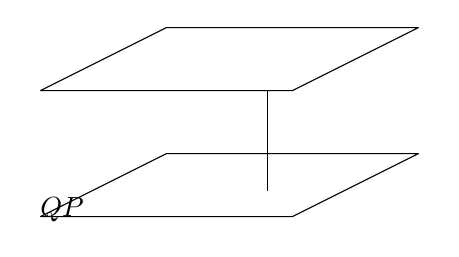
\begin{tikzpicture}[line join=round,scale=1.6]
	\clip (-0.1,-0.1) rectangle (3.1,1.5);
	\coordinate (A) at (0,0); 
	\coordinate (A') at (0,1);
	\coordinate (B) at (2,0);
	\coordinate (B') at (2,1);
	\coordinate (C) at (3,0.5);
	\coordinate (C') at (3,1.5);
	\coordinate (D) at (1,0.5);
	\coordinate (D') at (1,1.5);
	\coordinate (M) at (1.8,1.3);
	\coordinate (H) at (1.8,.2);
	\coordinate (E) at (1.8,1);
	\draw (A) -- (B) --(C) -- (D)--(A) (A') -- (B') -- (C')--(D')--(A');
	\draw (E) -- (H);
	\tkzDrawPoints[size=2](M,H)
	\tkzDrawSegment[dashed](M,E)
	\tkzLabelPoints[left](M,H)
	\tkzMarkAngle[mark=,size=0.7](B,A,D)
	\tkzLabelAngle[pos=-0.5](D,A,B){$Q$}
	\tkzMarkAngle[mark=,size=0.7](B',A',D')
	\tkzLabelAngle[pos=-0.5](D',A',B'){$P$}
	\end{tikzpicture}
\end{center}
\begin{boxdn}
	\begin{itemize}
	\item Khoảng cách giữa hai mặt phẳng song song $(P)$ và $(Q)$, kí hiệu $\mathrm{d}((P),(Q))$, là khoảng cách từ một điểm bất kì thuộc mặt phẳng này đến mặt phẳng kia.
	\item Khoảng cách giữa hai đường thẳng song song $m$ và $n$, kí hiệu $\mathrm{d}(m,n)$, là khoảng cách từ một điểm thuộc đường thẳng này đến đường thẳng kia.
	\end{itemize}
\end{boxdn}
\begin{boxdn}
	Khoảng cách giữa hai đáy của một hình lăng trụ được gọi là chiều cao của hình lăng trụ đó.
\end{boxdn}
\subsubsection{Khoảng cách giữa hai đường thẳng chéo nhau}
\begin{boxdn}
	\immini{Đường thẳng $\Delta$ cắt hai đường thẳng chớ nhau $a$, $b$ và vuông góc với cả hai đường thẳng đó được gọi là đường vuông góc chung của $a$ và $b$.\\
	Nếu đường vuông góc chung $\Delta$ cắt $a$, $b$ tương ứng tại $M$, $N$ thì độ dài đoạn $MN$ được gọi là khoảng cách giữa hai đường thẳng chéo nhau $a$, $b$.}{\begin{tikzpicture}[scale=1,font=\footnotesize,line join = round, line cap = round, >= stealth]
	%\draw[opacity=0.3] (0,0) grid (6,6);
	\def\x{3} \def\y{2} \def\z{4}
	\def\g{-120}
	\coordinate (A) at (0,2);
	\coordinate (B) at (4,4);
	\coordinate (C) at (0,1);
	\coordinate (D) at (4,0);
	\coordinate (E) at (2.5,4.5);
	\coordinate (F) at (2.5,0);
	\tkzInterLL(A,B)(E,F) \tkzGetPoint{M}
	\tkzInterLL(C,D)(E,F) \tkzGetPoint{N}
	\tkzMarkRightAngle(A,M,N)
	\tkzMarkRightAngle(D,N,M)
	\draw (A)--(B) (C)--(D) (E)--(F);
	\draw (A) node[above]{$a$} (C) node[below]{$b$} (E)node[right]{$\Delta$};
	\draw ($(M)+(160:0.3)$)node{$M$};
	\draw ($(N)+(-140:0.3)$)node{$N$};
	\foreach \p/\g in {M,N} \draw[fill] (\p) circle(.5pt)
	%node [shift={(\g:.3)}] {$\p$}
	;
	\end{tikzpicture}}
\end{boxdn}
\textbf{Nhận xét}
\begin{itemize}
	\item Khoảng cách giữa hai đường thẳng chéo nhau bằng khoảng cách giữa một trong hai đường thẳng đó đến mặt phẳng song song với nó và chứa đường thẳng còn lại.
	\item Khoảng cách giữa hai đường thẳng chéo nhau bằng khoảng cách giữa hai mặt phẳng song song tương ứng chứa hai đường thẳng đó.
\end{itemize}
\begin{minipage}[t]{0.5\textwidth}
	\begin{center}
	\begin{tikzpicture}[scale=1,font=\footnotesize,line join = round, line cap = round, >= stealth]
	%\draw[opacity=0.3] (0,0) grid (6,6);
	\def\x{4} \def\y{2} \def\z{4}
	\def\g{60}
	\coordinate (A) at (1,3);
	\coordinate (B) at (4,4.5);
	\coordinate (C) at (1,1.8);
	\coordinate (D) at (4,1);
	\coordinate (E) at (2.5,3.5);
	\coordinate (F) at (2.5,1);
	\tkzInterLL(A,B)(E,F) \tkzGetPoint{M}
	\tkzInterLL(C,D)(E,F) \tkzGetPoint{N}
	%%%
	\coordinate (a) at (0,.5);
	\coordinate (b) at ($(a)+(0:\x)$);
	\coordinate (d) at ($(a)+(\g:\y)$);
	\coordinate (c) at ($(b)+(d)-(a)$);
	\draw (a)--(b)--(c)--(d)--cycle;
	\begin{scope}
	\clip (b)--(a)--(d);
	\draw (a) circle (0.5);
	\draw ($(a)+(20:0.3)$)node[rotate=-15]{$P$};
	\end{scope}
	\tkzMarkRightAngle(A,M,N)
	\tkzMarkRightAngle(D,N,M)
	\draw (A)--(B) (C)--(D) (M)--(N);
	\draw (A) node[above]{$a$} (C) node[below]{$b$} ;
	\draw ($(M)+(160:0.3)$)node{$M$};
	\draw ($(N)+(-140:0.3)$)node{$N$};
	\foreach \p/\g in {M,N} \draw[fill] (\p) circle(.5pt)
	%node [shift={(\g:.3)}] {$\p$}
	;
	\end{tikzpicture}
	\end{center}
\end{minipage}\begin{minipage}[t]{0.5\textwidth}
	\begin{center}
	\begin{tikzpicture}[scale=1,font=\footnotesize,line join = round, line cap = round, >= stealth]
	%\draw[opacity=0.3] (0,0) grid (6,6);
	\def\x{4} \def\y{2} \def\z{4}
	\def\g{60}
	\coordinate (A) at (1,3);
	\coordinate (B) at (4,4);
	\coordinate (C) at (1,1.8);
	\coordinate (D) at (4,1);
	\coordinate (E) at (2.5,3.5);
	\coordinate (F) at (2.5,1);
	\tkzInterLL(A,B)(E,F) \tkzGetPoint{M}
	\tkzInterLL(C,D)(E,F) \tkzGetPoint{N}
	%%%
	\coordinate (a) at (0,.5);
	\coordinate (b) at ($(a)+(0:\x)$);
	\coordinate (d) at ($(a)+(\g:\y)$);
	\coordinate (c) at ($(b)+(d)-(a)$);
	\draw (a)--(b)--(c)--(d)--cycle;
	\begin{scope}
	\clip (b)--(a)--(d);
	\draw (a) circle (0.5);
	\draw ($(a)+(20:0.3)$)node[rotate=-15]{$P$};
	\end{scope}
	%%(Q)
	%%%
	\coordinate (a) at (0,2.7);
	\coordinate (b) at ($(a)+(0:\x)$);
	\coordinate (d) at ($(a)+(\g:\y)$);
	\coordinate (c) at ($(b)+(d)-(a)$);
	\tkzInterLL(a,b)(E,F) \tkzGetPoint{e}
	\draw[shift={(90:2)}] (a)--(b)--(c)--(d)--cycle;
	\draw[dashed] (M)--(e);
	\begin{scope}
	\clip (b)--(a)--(d);
	\draw (a) circle (0.5);
	\draw ($(a)+(30:0.3)$)node[rotate=0]{$Q$};
	\end{scope}
	\tkzMarkRightAngle(A,M,N)
	\tkzMarkRightAngle(D,N,M)
	\draw (A)--(B) (C)--(D) (e)--(N);
	\draw (A) node[above]{$a$} (C) node[below]{$b$} ;
	\draw ($(M)+(160:0.3)$)node{$M$};
	\draw ($(N)+(-140:0.3)$)node{$N$};
	\foreach \p/\g in {M,N} \draw[fill] (\p) circle(.5pt)
	%node [shift={(\g:.3)}] {$\p$}
	;
	\end{tikzpicture} 
	\end{center} 
\end{minipage}
\end{tomtat}
%%%%%%%%%%%%%%%%%%%
\subsection{Các dạng bài tập}
\begin{dang}{Khoảng cách từ một điểm đến một đường thẳng, đến một mặt phẳng}
\end{dang}
\subsubsection{Ví dụ minh hoạ}
\begin{vd}%[1C8Y5-2]
	\immini
	{
	Cho đoạn thẳng $M N$ có độ dài $a$ và đường thẳng $\Delta$ đi qua $N$ thoả mãn góc giữa hai đường thẳng $M N$ và $\Delta$ là $\varphi$ $\left(0^{\circ}<\varphi<90^{\circ}\right)$. Tính khoảng cách từ $M$ đến $\Delta$ theo $a$, $\varphi$.
	}
	{
	\begin{tikzpicture}[scale=.7,font=\footnotesize, line join=round, line cap=round, >=stealth]
	\tkzDefPoints{0/0/A,5/0/B}
	\coordinate (H) at ($(A)!.3!(B)$);
	\coordinate (N) at ($(A)!.8!(B)$);
	\coordinate (p) at ($(N)+(-0.9,0.4)$);
	\coordinate (a) at ($(M)!0.5!(N)$);
	\coordinate (M) at ($(H)+(0,3)$);
	\foreach \x/\g in {H/-90,M/90,N/-90} \fill[black](\x) circle (1.5pt) ($(\x)+(\g:3mm)$) node{$\x$};
	\draw (A)--(B)node[above]{$\Delta$}
	(M)--(H)
	(M)--(N)
	(a)node[above right]{$a$}
	(p)node{$\varphi$};
	\tkzMarkRightAngles[size=0.4](M,H,B)
	\tkzMarkAngles[size=.7cm,arc=l,mark=](M,N,A)
	\end{tikzpicture}
	}
	\loigiai{
	Gọi $H$ là hình chiếu của $M$ trên đường thẳng $\Delta$. Khi đó $\mathrm{d}(M, \Delta)=M H$.\\
	Vì góc giữa hai đường thẳng $M N$ và $\Delta$ là $\varphi$ nên $\widehat{M N H}=\varphi$.\\
	Suy ra $M H=M N \cdot \sin \varphi=a \sin \varphi$. Vậy $\mathrm{d}(M, \Delta)=a \sin \varphi$.
	}
\end{vd}
\begin{vd}%[1H3K5]
	Cho hình chóp $S.ABCD$ có đáy $ABCD$ là hình vuông cạnh $a$, tâm $O$, $SA=a$ và vuông góc với mặt phẳng $(ABCD)$. Gọi $I, M$ theo thứ tự là trung điểm của $SC, AB$.
	\begin{enumerate}
	\item Chứng minh $OI \perp (ABCD)$.
	\item Tính khoảng cách từ $I$ đến $CM$, từ đó suy ra khoảng cách từ $S$ tới $CM$.
	\end{enumerate}
	\loigiai{
	\immini{
	\begin{enumerate}
	\item Trong $\triangle{SAC}$, $OI$ là đường trung bình nên $OI \parallel SA \Rightarrow OI \perp (ABCD)$.
	\item Hạ $IH \perp CM$ tại $H$. Ta có $CM \perp (IOH)$ suy ra $CM \perp OH$.\\
	Gọi $K$ là trọng tâm tam giác $ABC$, ta có $OB=\dfrac{AC}{2}=\dfrac{a \sqrt 2}{2}; OK = \dfrac{OB}{3}=\dfrac{a \sqrt 2}{6}$.\\
	Trong $\triangle{OCK}: \dfrac{1}{OH^2}=\dfrac{1}{OK^2}+\dfrac{1}{OC^2} \Rightarrow OH=\dfrac{a}{\sqrt{20}}$.\\
	Trong $\triangle{OIH}: {IH^2}={OI^2}+{OH^2} \Rightarrow IH=\dfrac{a\sqrt{30}}{{10}}$.\\
	Ta có $SI \cap CM=C$ suy ra $\dfrac{\mathrm{d}(S, CM)}{\mathrm{d}(I, CM)}=\dfrac{SC}{IC}=2 \Rightarrow \mathrm{d}(S, CM)=\dfrac{a\sqrt{30}}{{5}}$
	\end{enumerate}	
	}
	{\begin{tikzpicture}[line join=round,scale=.8]
	\tkzDefPoints{0/0/A, -2/-2/B, 3/-2/C}
	\coordinate (D) at ($(A)+(C)-(B)$);
	\coordinate (S) at ($(A)+(0,5)$);
	\tkzInterLL(A,C)(B,D)\tkzGetPoint{O}
	\tkzDrawPolygon(S,C,D)
	\tkzDrawSegments(S,B B,C)
	\tkzDefMidPoint(B,A)\tkzGetPoint{M}
	\tkzDefMidPoint(S,C)\tkzGetPoint{I}
	\tkzDrawSegments[dashed](S,A A,B A,D A,C B,D O,I C,M)
	\tkzInterLL(M,C)(B,O)\tkzGetPoint{K}
	\tkzLabelPoints[left](A,B, M)
	\tkzLabelPoints[right](C,D)
	\tkzLabelPoints[above](S,I)
	\tkzLabelPoints[above right](O)
	\tkzLabelPoints[below right](K)
	\end{tikzpicture}}}
\end{vd}
\begin{vd}%[1T8B4-3]
	\immini
	{Cho hình chóp $O.ABC$ có đáy là tam giác đều cạnh $a$ và $OA\perp(ABC)$. Cho biết $OA=a$.
	\begin{enumerate}
	\item Tính khoảng cách từ điểm $O$ đến $(ABC)$.
	\item Tính khoảng cách từ điểm $O$ đến đường thẳng $BC$.
	\end{enumerate}
	}
	{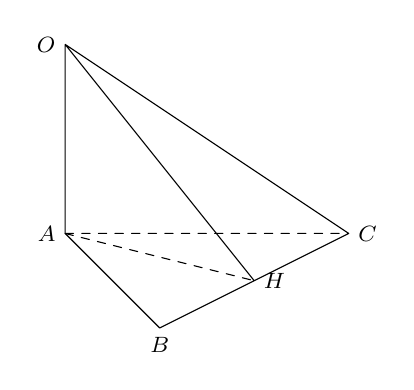
\begin{tikzpicture}[scale=0.6, font=\footnotesize, line join=round, line cap=round, >=stealth]
	\draw (0,0) node[left]{$A$};
	\draw (2,-2) node[below]{$B$};
	\draw (6,0) node[right]{$C$};
	\draw (4,-1) node[right]{$H$};
	\draw (0,4) node[left]{$O$};
	\coordinate (A) at (0,0);
	\coordinate (B) at (2,-2);
	\coordinate (C) at (6,0);
	\coordinate (H) at (4,-1);
	\coordinate (O) at (0,4);
	\draw (O)--(A)--(B)--(C)--(O)--(H);
	\draw[dashed] (A)--(C) (A)--(H);
	\tkzMarkRightAngle(O,A,C);
	\tkzMarkRightAngle(O,A,B);
	\tkzMarkRightAngle(C,H,O);
	\tkzMarkRightAngle(A,H,B);
	\end{tikzpicture}
	}
	\loigiai{
	\begin{enumerate}
	\item Ta có $OA\perp(ABC)$, suy ra $\mathrm{d}(O,(ABC))=OA=a$.
	\item Vẽ $AH\perp BC$, ta có $OH\perp BC$ (định lý ba đường vuông góc), \\
	suy ra $\mathrm{d}(O,BC)=OH$.\\
	Tam giác $ABC$ đều có cạnh bằng $a$ suy ra $AH=\dfrac{a\sqrt{3}}{2}$.\\
	Trong tam giác vuông $OAH$, ta có $OH=\sqrt{OA^2+AH^2}=\sqrt{a^2+\dfrac{3a^2}{4}}=\dfrac{a\sqrt{7}}{2}$.\\
	Vậy ta có $\mathrm{d}(O,BC)=\dfrac{a\sqrt{7}}{2}$.
	\end{enumerate}
	}
\end{vd}
\begin{vd}%[1H3B5]
	Cho hình chóp $S.ABC$ có $SA=a\sqrt{3}$, $SA\perp \left(ABC\right)$, tam giác $ABC$ vuông tại $B$ và $AB=a$. Tính khoảng cách từ điểm $A$ đến mặt phẳng $(SBC)$.
	\loigiai{
	\immini{
	Do $SA\perp \left(ABC\right)$ và $SA\subset \left(SAB\right)$ nên $\left(SAB\right)\perp \left(ABC\right)$. 
	Mà
	$\left(SAB\right)\cap \left(ABC\right)=AB$ và $AB\perp BC$ 
	nên $BC\perp \left(SAB\right)$. Do $BC\subset \left(SBC\right)$ 
	nên $\left(SBC\right)\perp \left(SAB\right)$. 
	Kẻ $AH\perp SB$ với $H\in SB$. 
	Do $\left(SAB\right)\cap \left(SBC\right)=SB$ nên $AH\perp \left(SBC\right)$ $\Rightarrow d\left(A,\left(SBC\right)\right)=AH$. 
	Do $SA\perp \left(ABC\right)$ nên $SA\perp AB$ 
	nên 
	$\dfrac{1}{AH^2}=\dfrac{1}{SA^2}+\dfrac{1}{AB^2}$
	$=\dfrac{1}{3a^2}+\dfrac{1}{a^2}=\dfrac{4}{3a^2}$.
	Vậy $d\left(A,\left(SBC\right)\right)=\dfrac{\sqrt{3}a}{2}$.
	}{
	\begin{tikzpicture}[line join=round,line cap=round,smooth, samples =100,>=stealth,scale=0.9]
	\tkzDefPoints{0/0/A, 1/-2/B, 4/0/C,0/3/S}
	\tkzLabelPoints[left](A)
	\tkzLabelPoints[above,right](B)
	\tkzLabelPoints[below](C)
	\tkzLabelPoints[above](S)
	\tkzDrawSegments(S,A S,B S,C A,B C,B)
	\tkzDrawSegments[dashed](A,C) 
	\coordinate (H) at ($(S)!0.33!(B)$);
	\tkzDrawSegments(A,H)
	\tkzMarkRightAngle(A,H,B)
	\tkzLabelPoints[above right](H)
	\end{tikzpicture}
	}
	}
\end{vd}
\begin{vd}%[1H3K5]
	Cho hình chóp $S.ABCD$ có tam giác $SAB$ đều và nằm trong mặt phẳng vuông góc với $\left(ABCD\right)$, tứ giác $ABCD$ là hình vuông cạnh $a$. Gọi $H$ là trung điểm của $AB$. Tính khoảng cách từ điểm $H$ đến mặt phẳng $(SCD).$
	\loigiai{
	\immini{
	Do tam giác $SAB$ đều và $H$ là trung điểm của $AB$ nên $SH\perp AB$. 
	Mà $\left(SAB\right)\perp \left(ABCD\right)$. 
	Nên $SH\perp \left(ABCD\right)$ $\Rightarrow SH\perp CD$. 
	Do $ABCD$ là hình vuông nên gọi $E$ là trung điểm của $CD$ nên $HE\perp CD$. 
	Vậy $CD\perp \left(SHE\right)$. 
	Mà $CD\subset \left(SCD\right)$ nên $\left(SCD\right)\perp \left(SHE\right)$. 
	Ta có $\left(SCD\right)\cap \left(SHE\right)=SE$. 
	Kẻ $HK\perp SE$ với $K\in SE$ nên $HK\perp \left(SCD\right)$.
	Khi đó $d\left(H,\left(SCD\right)\right)=HK$.
	Vì $AB=a$ nên $SH=\dfrac{\sqrt{3}a}{2}$. 
	Do $ABCD$ là hình vuông nên $HE=a$. 
	Vì $SH\perp \left(ABCD\right)$ nên $SH\perp HE$. }{
	\begin{tikzpicture}[line join=round,scale=.6]
	\tkzDefPoints{0/0/A, -2/-2/B, 3/-2/C}
	\coordinate (D) at ($(A)+(C)-(B)$);
	\coordinate (H) at ($(A)!0.5!(B)$);
	\coordinate (S) at ($(H)+(0,5)$);
	\coordinate (E) at ($(C)!.5!(D)$);
	\coordinate (K) at ($(S)!.6!(E)$);
	%\tkzInterLL(A,C)(B,D) %giao điểm AC với BD
	%\tkzGetPoint{O} %đặt tên giao điểm là $O$
	\tkzDrawSegments[dashed](S,A A,B A,D S,H H,E H,K)
	\tkzDrawPolygon(S,C,D)
	\tkzDrawSegments(S,B B,C S,E)
	\tkzLabelPoints[left](A,B)
	\tkzLabelPoints[right](C,D,K)
	\tkzLabelPoints[above](S)
	\tkzLabelPoints[below right](H,E)
	\tkzMarkRightAngle(H,K,E)
	\end{tikzpicture}
	} 
	Khi đó $\dfrac{1}{HK^2}=\dfrac{1}{SH^2}+\dfrac{1}{HE^2}$ $=\dfrac{7}{3a^2}$. Nên $HK=\dfrac{\sqrt{21}a}{7}$. 
	Vậy $d\left(H,\left(SCD\right)\right)=\dfrac{\sqrt{21}a}{7}$.	
	}
\end{vd}
\begin{vd}%[1H3K5]
	Cho hình chóp $S.ABC$ có đáy $ABC$ là tam giác vuông tại $A$, $AB=1, AC=\sqrt{3}$. Tam giác $SBC$ đều và nằm trong mặt phẳng vuông với đáy. Tính khoảng cách từ $B$ đến mặt phẳng $\left(SAC\right)$.
	\loigiai{
	\immini{
	Gọi $H$ là trung điểm của $BC$, \\ suy ra 
	$SH\perp BC\Rightarrow SH\perp \left(ABC\right)$.
	Gọi $K$ là trung điểm $AC$, suy ra $HK\perp AC$.	
	Kẻ $HE\perp SK\left(E\in SK\right).$
	Khi đó $d\left(B,\left(SAC\right)\right)=2d\left(H,\left(SAC\right)\right)$ \\
	$=2HE=2.\dfrac{SH.HK}{\sqrt{SH^2+HK^2}}=\dfrac{2\sqrt{39}}{13}.$
	}
	{ \begin{tikzpicture}[line join=round,line cap=round,smooth, samples =100,>=stealth,scale=0.9]
	\tkzDefPoints{0/0/A, 1/-2/B, 7/0/C,4/3/S}
	\coordinate (H) at ($(B)!0.5!(C)$);
	\coordinate (K) at ($(A)!0.5!(C)$);
	\coordinate (E) at ($(K)!0.5!(S)$);
	\tkzLabelPoints[left](A,E)
	%\tkzLabelPoints[above](B)
	\tkzLabelPoints[below](C,B)
	\tkzLabelPoints[above](S)
	\tkzDrawSegments(S,A S,B S,C A,B C,B S,H)
	\tkzDrawSegments[dashed](A,C A,H A,K H,K H,E S,K) 
	\tkzLabelPoints[right](H,K)
	\tkzMarkRightAngle[dashed](A,K,H)
	\tkzMarkRightAngle[dashed](S,E,H)
	\end{tikzpicture}
	}
	}
\end{vd}
\begin{vd}%[1H3K5]
	Cho hình chóp tứ giác đều $S.ABCD$ có cạnh bên là $2a$ và diện tích đáy là $4a^2$. Tính khoảng cách từ $A$ đến mặt phẳng $\left(SBC\right)$.
	\loigiai{
	\immini{
	Gọi $O=AC\cap BD\Rightarrow SO\perp \left(ABCD\right)$.
	Ta có $d\left(A,\left(SBC\right)\right)=2d\left[O,\left(SBC\right)\right]$.
	Kẻ $OE\perp BC,OF\perp SE$ ta có 
	$\heva{
	& BC\perp OE \\ 
	& BC\perp SO \\ 
	}\Rightarrow BC\perp \left(SOE\right)$ .
	$\Rightarrow BC\perp OF$ mà $OF\perp SE\Rightarrow OF\perp \left(SBC\right)$.
	Ta có $S_{ABCD}=AB^2=4a^2\Rightarrow AB=2a\Rightarrow OE=a$.
	Ta có $AC=2a\sqrt{2}\Rightarrow OA=a\sqrt{2}\Rightarrow SO=\sqrt{SA^2-OA^2}=a\sqrt{2}$.
	Ta có $\dfrac{1}{OF^2}=\dfrac{1}{OS^2}+\dfrac{1}{OE^2}=\dfrac{3}{2a^2}\Rightarrow OF=\dfrac{a\sqrt{6}}{3}$.
	$\Rightarrow d\left(O,\left(SBC\right)\right)=\dfrac{a\sqrt{6}}{3}\Rightarrow d\left(A,\left(SBC\right)\right)=\dfrac{2a\sqrt{6}}{3}$.
	}
	{
	\begin{tikzpicture}[line join=round,scale=.8]
	\tkzDefPoints{0/0/A, -2/-2/B, 3/-2/C}
	\coordinate (D) at ($(A)+(C)-(B)$);
	\tkzInterLL(A,C)(B,D) %giao điểm AC với BD
	\tkzGetPoint{O} %đặt tên giao điểm là $O$
	\coordinate (S) at ($(O)+(0,5)$);
	\coordinate (M) at ($(S)!.5!(B)$);
	\coordinate (N) at ($(S)!.5!(D)$);
	\coordinate (E) at ($(B)!.5!(C)$);
	\coordinate (F) at ($(S)!.5!(E)$);
	\tkzDrawSegments[dashed](S,A A,B A,D A,C B,D S,O O,F O,E)
	\tkzDrawPolygon(S,C,D)
	\tkzDrawSegments(S,B B,C S,E)
	\tkzLabelPoints[left](A,B)
	\tkzLabelPoints[right](C,D,O, E,F)
	\tkzLabelPoints[above](S)
	\end{tikzpicture}
	}
	}
\end{vd}
\begin{vd}%[1H3K5]
	Cho hình chóp $S.ABC$ có cạnh $SA=SB=SC=a$ và $SA, SB, SC$ đôi một vuông góc với nhau. Tính theo $a$ khoảng cách $h$ từ điểm $S$ đến mặt phẳng $\left(ABC\right).$
	\loigiai{
	\immini{
	Gọi $H$ là chân đường cao hạ từ $S$ xuống $\left(ABC\right)$ và $M=AH\cap BC.$
	Ta có $SH\perp (ABC)\Rightarrow SH\perp BC\Rightarrow BC\perp SH.$
	Lại có $\heva{
	& SA\perp SB \\ 
	& SA\perp SC \\ 
	}\Rightarrow SA\perp \left(SBC\right)\Rightarrow SA\perp BC\Rightarrow BC\perp SA.$
	Như vậy 
	$\heva{
	& BC\perp SH \\ 
	& BC\perp SA \\ 
	}\Rightarrow BC\perp \left(SAM\right)\Rightarrow BC\perp SM.$
	Từ $SA\perp \left(SBC\right)\Rightarrow SA\perp SM$
	Do đó $ \dfrac{1}{SH^2}=\dfrac{1}{SA^2}+\dfrac{1}{SM^2}=\dfrac{1}{SA^2}+\dfrac{1}{SB^2}+\dfrac{1}{SC^2}=\dfrac{3}{a^2}\Rightarrow h=\dfrac{a}{\sqrt{3}}.$
	}{
	\begin{tikzpicture}[line join=round,line cap=round,smooth, samples =100,>=stealth,scale=0.9]
	\tkzDefPoints{0/0/S, 1/-2/B, 4/0/C,0/3/A}
	\coordinate (M) ($(B)!0.5!(C)$);
	\coordinate (H) ($(A)!0.5!(M)$);
	\tkzCentroid(A,B,C)
	\tkzGetPoint{H}
	\tkzInterLL(A,H)(B,C)
	\tkzGetPoint{M}
	\tkzLabelPoints[above](A)
	\tkzLabelPoints[below](B)
	\tkzLabelPoints[below](C,M)
	\tkzLabelPoints[left](S)
	\tkzLabelPoints[right](H)
	\tkzDrawSegments(S,A S,B A,B C,B A,C A,M A,H B,M)
	\tkzDrawSegments[dashed](S,C S,M S,H) 
	\end{tikzpicture}
	}
	}
\end{vd}
\begin{vd}%[1H3K5]
	Cho hình chóp $S.ABCD$ có đáy $ABCD$ là hình vuông cạnh bằng $1$. Tam giác $SAB$ đều và nằm trong mặt phẳng vuông góc với đáy $\left(ABCD\right)$. Tính khoảng cách từ $A$ đến $\left(SCD\right)$.
	\loigiai{
	\immini{
	Gọi $H$ là trung điểm $AB$, suy ra $SH\perp AB.$ 
	Do đó $SH\perp \left(ABCD\right).$ 
	Do $AH\parallel CD$ nên $d\left(A,\left(SCD\right)\right)=d\left(H,\left(SCD\right)\right).$ 
	Gọi $E$ là trung điểm $CD$; $K$ là hình chiếu vuông góc của $H$ trên $SE$.
	Khi đó $d\left(H,\left(SCD\right)\right)=HK=\dfrac{SH.HE}{\sqrt{SH^2+HE^2}}=\dfrac{\sqrt{3}}{\sqrt{7}}.$ 
	Vậy $d\left(A,\left(SCD\right)\right)=HK=\dfrac{\sqrt{21}}{7}.$
	}{
	\begin{tikzpicture}[line join=round,scale=.65]
	\tkzDefPoints{0/0/A, -2/-2/B, 3/-2/C}
	\coordinate (D) at ($(A)+(C)-(B)$);
	\coordinate (H) at ($(A)!.5!(B)$);
	\coordinate (S) at ($(H)+(0,5)$);
	\coordinate (E) at ($(C)!.5!(D)$);
	\coordinate (K) at ($(S)!.3!(E)$);
	%\tkzInterLL(A,C)(B,D) %giao điểm AC với BD
	%\tkzGetPoint{O} %đặt tên giao điểm là $O$
	\tkzDrawSegments[dashed](S,A A,B A,D S,H H,E H,K)
	\tkzDrawPolygon(S,C,D)
	\tkzDrawSegments(S,B B,C S,E)
	\tkzLabelPoints[left](A,B,H)
	\tkzLabelPoints[right](C,D,E,K)
	\tkzLabelPoints[above](S)
	\end{tikzpicture}
	}
	}
\end{vd}
\subsubsection{Bài tập áp dụng}
\begin{bt}%[1H3K5]
	Cho hình lập phương $ABCD.A'B'C'D'$ có cạnh bằng $a$. Chứng minh rằng khoảng cách từ điểm $B, C, D, A', B', D'$ đến đường chéo $AC'$ đều bằng nhau. Tính khoảng cách đó.
	\loigiai{Ta có $\triangle{BAC'}=\triangle{CA'A}=\triangle{DAC'}=\triangle{A'AC}=\triangle{B'C'A}=\triangle{D'C'A}$ chung đáy $AC'$ nên khoảng cách từ $B, C, D, A', B', D'$ đến đường chéo $AC'$ đều bằng nhau.\\
	Hạ $CH \perp AC'$, ta được $\dfrac{1}{CH^2}=\dfrac{1}{AC^2}+\dfrac{1}{C'C^2} \Rightarrow CH=\dfrac{a \sqrt 6}{3}$.
	}
\end{bt}
\begin{bt}%[1K7BP-3]
	Cho hình chóp đều $S.ABC$. Biết độ dài cạnh đáy, cạnh bên tương ứng bằng $a$, $b$ ($a<b\sqrt{3}$). Tính chiều cao của hình chóp.
	\loigiai{
	\immini{
	Hình chiếu của $S$ trên mặt phẳng $(ABC)$ là tâm $O$ của tam giác đều $ABC$. \\
	Trong tam giác đều $ABC$, ta có $OA=\dfrac{a}{\sqrt{3}}$. \\
	Trong tam giác vuông $SOA$, ta có \[SO=\sqrt{SA^2-OA^2}=\sqrt{b^2-\dfrac{a^2}{3}}.\]
	Vậy chiều cao của hình chóp là $SO=\sqrt{b^2-\dfrac{a^2}{3}}$.
	}{
	\begin{tikzpicture}[scale=1, font=\footnotesize, line join=round, line cap=round, >=stealth]
	\tkzDefPoints{0/0/A,5/0/C,1.2/-1.5/B,0/3/x}
	\coordinate (I) at ($(B)!0.5!(C)$);
	\coordinate (O) at ($(A)!2/3!(I)$);
	\coordinate (S) at ($(O)+(x)$);
	\tkzDrawSegments(S,A S,B S,C A,B B,C)
	\tkzDrawSegments[dashed](S,O A,O A,C)
	\foreach \x/\g in {A/180,B/-90,C/0,S/90,O/-60} \fill[black] (\x) circle (1pt) +(\g:0.3)node{$\x$};
	\tkzMarkRightAngle(S,O,A)
	\end{tikzpicture}
	}
	}
\end{bt}
\begin{bt}%[1H3B5]
	Cho tứ diện $S.ABC$ có đáy $ABC$ là tam giác đều cạnh $a\sqrt{3}.$ Cạnh $SA=2a$ là vuông góc với mặt phẳng đáy. Tính khoảng cách $d$ từ điểm $A$ đến mặt phẳng $\left(SBC\right).$
	\loigiai{
	\immini{
	Tam giác $ABC$ đều, kẻ $AM\perp BC \left(M\in BC\right)\Rightarrow M$ là trung điểm của cạnh $BC.$
	Ta có $\heva{
	& BC\perp AM \\ 
	& BC\perp SA \\ 
	}\Rightarrow BC\perp \left(SAM\right).$
	Khi đó kẻ 
	$AH\perp SM \left(H\in SM\right)\Rightarrow BC\perp AH.$
	Như vậy 
	$\heva{
	& AH\perp SM \\ 
	& AH\perp BC \\ 
	}\Rightarrow AH\perp \left(SBC\right)\Rightarrow d=d\left(A;\left(SBC\right)\right)=AH.$
	Ta có
	$AM=\dfrac{AB\sqrt{3}}{2}=\dfrac{3a}{2}\Rightarrow \dfrac{1}{AH^2}=\dfrac{1}{SA^2}+\dfrac{1}{AM^2} =\dfrac{1}{4a^2}+\dfrac{1}{\left(\dfrac{3a}{2}\right)^2}=\dfrac{25}{36a^2}$
	$\Rightarrow AH=\dfrac{6}{5}a\Rightarrow d=\dfrac{6}{5}a.$
	}
	{ \begin{tikzpicture}[line join=round,line cap=round,smooth, samples =100,>=stealth,scale=0.9]
	\tkzDefPoints{0/0/A, 1.5/-2/B, 4.5/0/C}
	\coordinate (S) at ($(A)+(0,4)$);
	\coordinate (M) at ($(B)!0.5!(C)$);
	\coordinate (H) at ($(S)!0.4!(M)$);
	\tkzLabelPoints[left](A)
	\tkzLabelPoints[below](B)
	\tkzLabelPoints[right](C,H,M)
	\tkzLabelPoints[above](S)
	\tkzDrawSegments(S,A S,B S,C A,B C,B S,M)
	\tkzDrawSegments[dashed](A,C A,M A,H) 
	\end{tikzpicture}
	}
	}
\end{bt}
\begin{bt}%[1H3B5]
	Cho hình chóp tam giác $S.ABC$ có $AB=BC=2a$ và $\widehat{ABC}=120^{\circ}.$ Cạnh $SA=3a$ và vuông góc với mặt phẳng đáy. Tính khoảng cách $d$ cách từ $A$ đến mặt phẳng $\left(SBC\right).$
	\loigiai{
	\immini{
	Kẻ $AM\perp BC \left(M\in BC\right),$ ta có
	$\heva{
	& CM\perp SA \\ 
	& CM\perp AM \\ 
	} \Rightarrow CM\perp \left( SAM \right) \Rightarrow CM \perp AM.$
	Ta có $AM =2a \sin 60^{\circ}=a\sqrt{3}$
	Xét $\triangle SAM$ ta có $\dfrac{1}{d^2} =\dfrac{1}{AH^2} =\dfrac{1}{SA^2}+\dfrac{1}{AM^2}\Rightarrow d= \dfrac{3a}{2}$
	}{
	\begin{tikzpicture}[line join=round,line cap=round,smooth, samples =100,>=stealth,scale=0.6]
	\tkzDefPoints{0/0/A, 3.5/-2/B, 4.5/0/C}
	\coordinate (S) at ($(A)+(0,4)$);
	\coordinate (M) at ($(B)!-0.5!(C)$);
	\coordinate (H) at ($(S)!0.3!(M)$);
	\tkzLabelPoints[left](A,H)
	\tkzLabelPoints[below](B)
	\tkzLabelPoints[right](C,M)
	\tkzLabelPoints[above](S)
	\tkzDrawSegments(S,A S,B S,C A,M C,B S,M A,H B,M)
	\tkzDrawSegments[dashed](A,C A,B) 
	\end{tikzpicture}
	}
	}
\end{bt}
\begin{bt}%[1H3B5]
	Cho hình chóp $S.ABCD$ có đáy $ABCD$ là hình chữ nhật có $AB=a\sqrt{2}$. Cạnh bên $SA=2a$ và vuông góc với mặt đáy $\left(ABCD\right)$. Tính khoảng cách từ $D$ đến mặt phẳng $\left(SBC\right)$.
	\loigiai{
	\immini{
	Do $AD\parallel BC$ nên $d\left(D,\left(SBC\right)\right)=d\left(A,\left(SBC\right)\right)$.
	Gọi $K$ là hình chiếu của $A$ trên $SB$, suy ra $AK\perp SB$. 
	Khi $d\left[A,\left(SBC\right)\right]=AK=\dfrac{SA.AB}{\sqrt{SA^2+AB^2}}=\dfrac{2a\sqrt{3}}{3}.$
	}
	{
	\begin{tikzpicture}[line join=round,scale=.55]
	\tkzDefPoints{0/0/A, -2/-2/B, 3/-2/C}
	\coordinate (D) at ($(A)+(C)-(B)$);
	\coordinate (S) at ($(A)+(0,5)$);
	\coordinate (K) at ($(S)!.5!(B)$);
	\coordinate (N) at ($(S)!.5!(D)$);
	%\tkzInterLL(A,C)(B,D) %giao điểm AC với BD
	%\tkzGetPoint{O} %đặt tên giao điểm là $O$
	\tkzDrawSegments[dashed](S,A A,B A,D A,K)
	\tkzDrawPolygon(S,C,D)
	\tkzDrawSegments(S,B B,C)
	\tkzLabelPoints[left](A,B,K)
	\tkzLabelPoints[right](C,D)
	\tkzLabelPoints[above](S)
	\end{tikzpicture}
	}
	}
\end{bt}
\begin{bt}%[1H3K5]
	Cho hình chóp $S.ABCD$ có đáy là hình vuông cạnh $a$; $SA$ vuông góc với đáy; $SB$ hợp với đáy góc $45^{\circ}$. Tính khoảng cách từ điểm $C$ đến mặt phẳng $\left(SBD\right).$
	\loigiai{
	\immini{
	Ta có $45^{\circ}=\widehat{ SB,(ABCD)}=\widehat{SBA}\Rightarrow SA=AB=a.$ 
	Gọi $O$ là giao điểm của $AC$ với $BD.$ 
	Ta có $d\left(C,\left(SBD\right)\right)=d\left(A,\left(SBD\right)\right).$ 
	Kẻ $AH\perp SO$ ta có 
	$\heva{
	& BD\perp AC \\ 
	& BD\perp SA \\ 
	}\Rightarrow BD\perp \left(SAC\right)$
	$\Rightarrow BD\perp AH$
	mà $AH\perp SO\Rightarrow AH\perp \left(SBD\right)$.
	Ta có $\dfrac{1}{AH^2}=\dfrac{1}{AO^2}+\dfrac{1}{AS^2}=\dfrac{3}{a^2}\Rightarrow AH=\dfrac{a}{\sqrt{3}}$.
	$\Rightarrow d\left(C,\left(SBD\right)\right)=\dfrac{a}{\sqrt{3}}$.
	}
	{
	\begin{tikzpicture}[line join=round,scale=.65]
	\tkzDefPoints{0/0/A, -2/-2/B, 3/-2/C}
	\coordinate (D) at ($(A)+(C)-(B)$);
	\coordinate (S) at ($(A)+(0,5)$);
	\coordinate (M) at ($(S)!.5!(B)$);
	\coordinate (H) at ($(S)!.5!(O)$);
	\tkzInterLL(A,C)(B,D) %giao điểm AC với BD
	\tkzGetPoint{O} %đặt tên giao điểm là $O$
	\tkzDrawSegments[dashed](S,A A,B A,D A,C B,D S,O A,H)
	\tkzDrawPolygon(S,C,D)
	\tkzDrawSegments(S,B B,C)
	\tkzLabelPoints[left](A,B)
	\tkzLabelPoints[right](C,D)
	\tkzLabelPoints[below right](O,H)
	\tkzLabelPoints[above](S)
	\end{tikzpicture}
	}
	}
\end{bt}
\begin{bt}%[1H3K5]
	Cho hình chóp $S.ABC$ có đáy $ABC$ là một tam giác đều cạnh $a$, cạnh $SA$ vuông góc với $\left(ABC\right)$ và $SA=h$, góc giữa hai mặt phẳng $\left(SBC\right)$ và $\left(ABC\right)$ bằng $60^{\circ}$. Tính khoảng cách từ $A$ đến $\left(SBC\right)$ theo $a$ và $h$.
	\loigiai{
	\immini{
	Gọi $I$ là trung điểm của $BC$, ta có $\heva{
	& AI\perp BC \\ 
	& SA\perp BC \\ 
	}\Rightarrow \left(SAI\right)\perp BC$
	Vậy $\widehat{AIS}$ chính là góc giữa hai mặt phẳng $\left(SBC\right)$ và $\left(ABC\right)$
	$\Rightarrow \widehat{AIS}=60^{\circ}$.
	Trong $\left(SBC\right)$kẻ $AH\perp SI$.
	Ta có $\heva{
	& BC\perp \left(SAI\right) \\ 
	& AH\subset \left(SAI\right) \\ 
	}\Rightarrow AH\perp BC$.
	Vậy $\heva{
	& AH\perp BC \\ 
	& AH\perp SI \\ 
	}\Rightarrow AH\perp \left(SBC\right)$
	$\Rightarrow d\left(A,\left(SBC\right)\right)=AH$.
	Tam giác $ABC$ đều cạnh $a$ nên $AI=\dfrac{a\sqrt{3}}{2}$
	Trong tam giác $AIS$ ta có 
	$\dfrac{1}{AH^2}=\dfrac{1}{AI^2}+\dfrac{1}{AS^2}=\dfrac{1}{{\left(\dfrac{a\sqrt{3}}{2}\right)}^2}+\dfrac{1}{h^2}=\dfrac{4h^2+3a^2}{3a^2h^2}$
	}
	{
	\begin{tikzpicture}[line join=round,line cap=round,smooth, samples =100,>=stealth,scale=0.9]
	\tkzDefPoints{0/0/A, 1.5/-2/B, 4.5/0/C}
	\coordinate (S) at ($(A)+(0,4)$);
	\tkzDefMidPoint(C,B)
	\tkzGetPoint{I}
	\tkzDefPointBy[projection= onto S--I](A)
	\tkzGetPoint{H}
	\tkzLabelPoints[left](A)
	\tkzLabelPoints[below](B)
	\tkzLabelPoints[right](C,H,I)
	\tkzLabelPoints[above](S)
	\tkzDrawSegments(S,A S,B S,C A,B C,B S,I)
	\tkzDrawSegments[dashed](A,C A,I A,H) 
	\end{tikzpicture}
	}
	$\Rightarrow AH=\dfrac{ah\sqrt{3}}{\sqrt{4h^2+3a^2}}$.
	\\
	Hay $d\left(A,\left(SBC\right)\right)=\dfrac{ah\sqrt{3}}{\sqrt{4h^2+3a^2}}$.
	}
\end{bt}
\begin{bt}%[1H3K5]
	Cho hình hộp $ABCD.A'B'C'D'$ có tất cả các mặt đều là hình thoi cạnh $a$, các góc $\widehat{BAA'}=\widehat{BAD}=\widehat{DAA'}=60^{\circ}$. Tính khoảng cách từ $A'$ đến $\left(ABCD\right)$.
	\loigiai{
	Do $ABCD.A'B'C'D'$ có tất cả các mặt đều là hình thoi cạnh $a$ và $\widehat{BAA'}=\widehat{BAD}=\widehat{DAA'}=60^{\circ}$ nên các tam giác $ABA',ABD,ADA'$ đều là các tam giác đều cạnh $a$
	$\Rightarrow A'A=A'B=A'D$ ($A'$ cách đếu ba đỉnh của $\triangle ABD$).
	\begin{center}
	\begin{tikzpicture}[line join=round,line cap=round,smooth, samples =100,>=stealth,scale=0.6]
	\tkzInit[xmin=-1,xmax=12,ymin=-1,ymax=8] 
	\tkzClip
	\tkzDefPoints{0/0/B, 6/0/C, 2/2/A}
	\tkzDefPointBy[translation = from B to C](A)
	\tkzGetPoint{D} 
	\tkzCentroid(A,B,D)
	\tkzGetPoint{H}
	\coordinate (A') at ($(H)+(0,5)$);
	\tkzDefPointBy[translation = from A to A'](B)
	\tkzGetPoint{B'}
	\tkzDefPointBy[translation = from A to A'](C)
	\tkzGetPoint{C'}
	\tkzDefPointBy[translation = from A to A'](D)
	\tkzGetPoint{D'}
	\tkzInterLL(A,C)(B,D)
	\tkzGetPoint{O}
	\tkzLabelPoints[left](A)
	\tkzLabelPoints[below](B,O)
	\tkzLabelPoints[right](C,D,C',D',H)
	\tkzLabelPoints[above](A',B')
	\tkzDrawPolygon(A',B',C',D')
	\tkzDrawSegments(B',B C',C C,B A',B' B',C' D,D' C,D)
	\tkzDrawSegments[dashed](A,D A,B A,A' A,B B,D A',H H,A H,B H,D A,C) 
	\end{tikzpicture}
	\end{center}
	Gọi $H$ là hình chiếu của $A'$ trên $\left(ABCD\right)$ thì các tam giác vuông $A'HA,A'HB,A'HD$ bằng nhau nên 
	$$HA=HB=HD.$$
	Do đó $H$ là tâm của đường tròn ngoại tiếp $\triangle ABD$.
	Gọi $O$ giao điểm của $AC$ và $BD$, ta có 
	$AH=\dfrac{2}{3}AO=\dfrac{2}{3}.\dfrac{a\sqrt{3}}{2}=\dfrac{a\sqrt{3}}{3}$.
	\begin{align*}
	A'H&=\sqrt{AA{'}^2-AH^2}\\&=\sqrt{a^2-{\left(\dfrac{a\sqrt{3}}{3}\right)}^2} \\ 
	& =a\sqrt{\dfrac{2}{3}}. \\ 
	\end{align*}
	Vậy $d\left(A',\left(ABCD\right)\right)=A'H=a\sqrt{\dfrac{2}{3}}$.
	}
\end{bt}
%-----------------
\begin{dang}{Khoảng cách giữa ĐT và MP song song, giữa hai MP song song}
\end{dang}
\subsubsection{Ví dụ minh hoạ}
\begin{vd}%[1K7BP-3]
	Cho một hình hộp đứng $ABCD.A'B'C'D'$, đáy là các hình thoi có cạnh bằng $a$, $\widehat{BAD}=120^\circ$, $AA'=h$. Tính các khoảng cách giữa $A'C'$ và $(ABCD)$, $AA'$ và $(BDD'B')$.
	\loigiai{
	\immini{
	Đường thẳng $A'C'$ thuộc mặt phẳng $(A'B'C'D')$ nên nó song song với mặt phẳng $(ABCD)$. Do $ABCD.A'B'C'D'$ là hình hộp đứng nên $A'A \perp(ABC D)$.\\	
	Vậy $\mathrm{d}\left(A'C',(ABC D)\right)=\mathrm{d}(A',(ABCD))=A'A=h$.\\
	Do $AA'$ song song với $BB'$ nên $AA'$ song song với $(BDD'B')$.
	}{
	\begin{tikzpicture}[scale=0.85, font=\footnotesize, line join=round, line cap=round, >=stealth]
	\tkzDefPoints{0/0/A,3/0/D,-1.5/-1.2/B,0/2.5/x}
	\coordinate (C) at ($(D)-(A)+(B)$);
	\coordinate (A') at ($(A)+(x)$);
	\coordinate (B') at ($(B)+(x)$);
	\coordinate (C') at ($(C)+(x)$);
	\coordinate (D') at ($(D)+(x)$);
	\coordinate (O) at ($(A)!0.5!(C)$);
	\tkzDrawSegments(B,B' C,C' D,D' B,C C,D A',B' B',C' C',D' D',A' A',C' B',D')
	\tkzDrawSegments[dashed](A,A' A,B A,D A,C B,D)
	\foreach \x/\g in {A/150,B/-150,C/-30,D/30,A'/150,B'/-150,C'/-30,D'/30,O/-90} \fill[black] (\x) circle (1pt) +(\g:0.3)node{$\x$};
	\end{tikzpicture}
	}
	Gọi $O$ là tâm của hình thoi $ABCD$. Do $AO\perp BD$ và $AO\perp BB'$ nên $AO \perp(BDD'B')$. Vậy khoảng cách giữa $AA'$ và $(BDD'B')$ bằng độ dài đoạn thẳng $AO$.\\
	Tam giác $BAD$ cân tại $A$ và có $\widehat{BAD}=120^\circ$ nên $\widehat{ABO}=30^\circ$.\\
	Do đó, trong tam giác vuông $AOB$, ta có $AO=\dfrac{AB}{2}=\dfrac{a}{2}$.\\
	Vậy khoảng cách giữa $AA'$ và $(BDD'B')$ bằng $\dfrac{a}{2}$.
	}
\end{vd}
\begin{vd}%[1C8B5-3]
	\immini
	{
	Cho hình chóp $S. A B C D$ có đáy $A B C D$ là hình vuông cạnh $a$, $O$ là giao điểm của $A C$ và $B D$, $S O \perp(A B C D)$, $S O=a$. Tính
	\begin{enumerate}
	\item Khoảng cách từ điểm $S$ đến mặt phẳng $(A B C D)$;
	\item Khoảng cách từ điểm $B$ đến mặt phẳng $(S A C)$.
	\end{enumerate}
	}
	{
	\begin{tikzpicture}[scale=.6,font=\footnotesize, line join=round, line cap=round, >=stealth]
	\tkzDefPoints{0/0/A,5/0/D,-2/-2/B}
	\coordinate (C) at ($(B)+(D)-(A)$);
	\coordinate (O) at ($(A)!.5!(C)$);
	\coordinate (S) at ($(O)+(0,5)$);
	\foreach \x/\g in {A/160,B/-100,C/-60,D/20,S/90,O/-90} \fill[black](\x) circle (1.5pt) ($(\x)+(\g:3mm)$) node{$\x$};
	\draw (S)--(B)--(C)--(D)--(S)--(C);
	\draw[dashed] (B)--(A)--(D)--(B)
	(O)--(S)--(A)--(C);
	\end{tikzpicture}
	}
	\loigiai{
	\begin{enumerate}
	\item Ta có $O \in(A B C D)$, $S O \perp(A B C D)$. Suy ra khoảng cách từ điểm $S$ đến mặt phẳng $(A B C D)$ là $S O=a$.
	\item Do $S O \perp(A B C D)$, $B O \subset(A B C D)$ nên $S O \perp B O$. Vì $B O$ vuông góc với hai đường thẳng $A C$ và $S O$ cắt nhau trong $(S A C)$ nên $B O \perp(S A C)$. Do $O \in(S A C)$, $B O \perp(S A C)$ nên khoảng cách từ $B$ đến mặt phẳng $(S A C)$ là $B O=\dfrac{a \sqrt{2}}{2}$. 
	\end{enumerate}
	}
\end{vd}
\begin{vd}%[1C8B5-2]
	\immini
	{
	Cho hình hộp $A B C D. A' B' C' D'$ có $A A'=a$, góc giữa hai đường thẳng $A B$ và $D D'$ bằng $60^{\circ}$. Tính khoảng cách giữa hai đường thẳng $A B$ và $A' B'$.
	}
	{
	\begin{tikzpicture}[scale=.45,font=\footnotesize, line join=round, line cap=round, >=stealth]
	\tkzDefPoints{0/0/A,5/0/B,2/2/D}
	\coordinate (C) at ($(B)+(D)-(A)$);
	\coordinate (H) at ($(A)!.2!(B)$);
	\coordinate (A') at ($(H)+(0,5)$);
	\coordinate (B') at ($(B)+(A')-(A)$);
	\coordinate (C') at ($(C)+(A')-(A)$);
	\coordinate (D') at ($(D)+(A')-(A)$);
	\foreach \x/\g in {A/-100,B/-60,C/-20,D/170,A'/170,B'/-10,C'/60,D'/100,H/-90} \fill[black](\x) circle (1.5pt) ($(\x)+(\g:3mm)$) node{$\x$};
	\draw (A')--(A)--(B)--(C)--(C')--(D')--(A')--(H)
	(A')--(B')--(C')
	(B)--(B');
	\draw[dashed] (A)--(D)--(C)
	(D')--(D);
	\tkzMarkRightAngles[size=0.4](A',H,B)
	\end{tikzpicture}
	}
	\loigiai{
	Gọi $H$ là hình chiếu vuông góc của $A'$ trên $A B$. Do $A B \parallel A' B'$ nên $\mathrm{d}\left(A B, A' B'\right)=A' H$.\\
	Vì $A A' \parallel D D'$ nên góc giữa đường thẳng $A B$ và $A A'$ bằng góc giữa đường thẳng $A B$ và $D D'$.\\
	Suy ra $\widehat{A' A H}=60^{\circ}$.\\
	Trong tam giác vuông $H A A'$ có $A' H=A A' \cdot \sin \widehat{A' A H}=a \sin 60^{\circ}=\dfrac{a \sqrt{3}}{2}$.\\
	Vậy $\mathrm{d}\left(A B, A' B'\right)=\dfrac{a \sqrt{3}}{2}$.
	}
\end{vd}
\begin{vd}%[1H3G5]
	Cho hình chóp $S.ABCD$ có $SA=a \sqrt 6$ và vuông góc với mặt phẳng $(ABCD)$, đáy $(ABCD)$ là nửa lục giác đều nội tiếp trong đường tròn đường kính $AD=2a$.
	\begin{enumerate}
	\item Tính khoảng cách từ $A, B$ đến mặt phẳng $(SCD)$.
	\item Tính khoảng cách từ đường thẳng $AD$ đến mặt phẳng $(SBC)$.
	\item Tính diện tích thiết diện của hình chóp $S. ABCD$ với mặt phẳng $(\alpha)$ song song với mặt phẳng $(SAD)$ và cách $(SAD)$ một khoảng bằng $\dfrac{a \sqrt 3}{4}$.
	\end{enumerate}
	\loigiai{	
	\begin{enumerate}
	\item \immini{Ta có $(SCD) \perp (SAC)$. Hạ $AH \perp SC \Rightarrow AH \perp (SCD)$. Suy ra $AH$ là khoảng cách từ $A$ tới $(SCD)$.\\
	Xét $\triangle{SAB}: \dfrac{1}{AH^2}=\dfrac{1}{AC^2}+\dfrac{1}{SA^2} \Rightarrow AH = a \sqrt 2$.\\
	Gọi $I$ là trung điểm của $AD$, suy ra
	\[BI \parallel CD \Rightarrow BI \parallel (SCD) \Rightarrow \mathrm{d}(B, (SCD))=\mathrm{d}(I, (SCD)).\]
	Mặt khác, $AI \cap (SCD)=D$, nên $\dfrac{\mathrm{d}(I, (SCD))}{\mathrm{d}(A, (SCD))}=\dfrac{ID}{AD}=\dfrac{1}{2}$.\\
	Suy ra $\mathrm{d}(I, (SCD))=\dfrac{a \sqrt 2}{2}$.
	}{	\begin{tikzpicture}[line join=round,scale=0.65]
	\tkzInit[xmin=-4,xmax=5,ymin=-3,ymax=5] 
	\tkzClip
	\tkzDefPoints{-3/0/A, -1/-2/B, 1/-2/C, 3/0/D, 3/0/D, 0/0/I, -3/4/S}
	% Ký hiệu điểm
	\tkzDrawPoints(A,B,S,C,D,I)
	\tkzDrawSegments(S,A A,B B,C C,D S,D S,B S,C) % Kẻ đoạn thẳng
	\tkzDrawSegments[dashed](A,D B,I) 
	\coordinate (H) at ($(S)!(A)!(C)$);
	\tkzDrawSegments(A,H)
	%	\tkzDrawAltitude[dashed](S,C)(A)\tkzGetPoint{H}
	%gán nhãn
	\tkzLabelPoints[above left](S)
	\tkzLabelPoints[left](A)
	\tkzLabelPoints[below](B,C)
	\tkzLabelPoints[right](D)
	\tkzLabelPoints[above right](I,H)
	\tkzMarkRightAngle(A,H,C)	
	\end{tikzpicture}}
	\item Ta có $AD \parallel CD \Rightarrow AD \parallel (SBC) \Rightarrow \mathrm{d}(AD, (SBC))=\mathrm{d}(A, (SBC))$.\\
	Hạ $AK \perp BC$, ta có $BC \perp (SAK) \Rightarrow (SBC)\perp (SAK)$ và $(SBC) \perp (SAK)=AK$.\\
	Hạ $AG \perp SK$, suy ra $AG \perp (SBC)$.\\
	Xét $\triangle{SAK}$, ta có 
	\[\dfrac{1}{AG^2}=\dfrac{1}{SA^2}+\dfrac{1}{AK^2}\Rightarrow AG =\dfrac{a \sqrt 6}{3}. \]
	\item Ta có $AK \perp (SAD)$. Giả sử $(\alpha) \parallel (SAD)$ cắt $AK$ tại $E$, khi đó
	\[\mathrm{d}((\alpha), (SAD))=AE=\dfrac{a \sqrt 3}{4}=\dfrac{1}{2}AK.\]
	Suy ra $E$ là trung điểm của $AK$. Ta xác định thiết diện của hình chóp với mặt phẳng $(\alpha)$ qua $E$ và song song với $(SAD)$.\\
	Thiết diện là hình thang vuông $MNPQ$ với $M, N, Q, P$ là trung điểm của $AB, CD, SB, SC$. Ta tính được $\mathcal{S}_{MNPQ}=\dfrac{a^2 \sqrt 6}{2}$.
	\end{enumerate}
	}
\end{vd}
\begin{vd}%[1H3K5]
	Cho hình hộp $ABCD. A'B'C'D'$ có các cạnh đều bằng $a$ và $\widehat{BAD}=\widehat{BAA'}=\widehat{DAA'}=60^\circ$. Tính khoảng cách giữa hai mặt phẳng đáy $(ABCD)$ và $A'B'C'D'$.
	\loigiai{
	\immini{Hạ $A'H \perp AC$. Ta có $BD \perp (OAA')$ suy ra $BD \perp A'H \Rightarrow A'H \perp (ABCD)$. Do $(ABCD) \parallel (A'B'C'D)$ nên $A'H$ là khoảng cách giữa hai mặt đáy. \\
	$A'.ABD$ là hình chóp đều nên $AH=\dfrac{2}{3}AO=\dfrac{a\sqrt 3}{3}$.
	\[A'H^2=A'A^2-AH^2=\dfrac{2a^2}{3} \Rightarrow A'H=\dfrac{a \sqrt 6}{3}.\]
	}
	{\begin{tikzpicture}[line join=round,scale=.6]
	\tkzDefPoints{-1/-2/x, 6/0/y, -1/3/z, 0/0/A}
	\coordinate (B) at ($(A)+(x)$);
	\coordinate (C) at ($(B)+(y)$);
	\coordinate (D) at ($(C)-(x)$);
	\coordinate (A') at ($(A)+(z)$);
	\coordinate (B') at ($(B)+(z)$);
	\coordinate (C') at ($(C)+(z)$);
	\coordinate (D') at ($(D)+(z)$);
	\tkzDrawSegments[dashed](B,A A,D A,A' A,C B,D A',D)
	\tkzInterLL(A,C)(B,D)\tkzGetPoint{O}
	\tkzDrawSegments(D,C D,D')
	\tkzDrawPolygon(A',B',C',D')
	\tkzDrawPolygon(B,B',C',C)
	\tkzLabelPoints[right](C, C', D', D)
	\tkzLabelPoints[left](A, B, A', B')
	\tkzLabelPoints[below](O)
	\end{tikzpicture}}	
	}
\end{vd}
\begin{vd}%[1H3K5]
	Cho hình chóp $S. ABC$ có đáy $ABC$ là tam giác đều cạnh bằng $a$, mặt bên $(SBC)$ vuông góc với đáy. Gọi $M, N, P$ theo thứ tự là trung điểm $AB, SA, AC$. Tính khoảng cách giữa hai mặt phẳng $(MNP)$ và $(SBC)$.
	\loigiai{
	\immini{Ta chứng minh được $(MNP) \parallel (SBC)$.\\
	Suy ra $\mathrm{d}((MNP); (SBC))=\mathrm{d}(P; (SBC))$.\\
	$AP \cap (SBC)=C$ suy ra $\mathrm{d}(P; (SBC))=\dfrac{AP}{AC}\mathrm{d}(A; (SBC))=\dfrac{1}{2}\mathrm{d}(A; (SBC))$.\\
	Gọi $K$ là trung điểm của $BC$. Tam giác $ABC$ đều suy ra $AK \perp BC$.
	\\ Do $(ABC)\perp (SBC)$ theo giao tuyến $BC$ nên $AK \perp (SBC)$.\\
	Do đó, $\mathrm{d}(A; (SBC))=AK =\dfrac{a\sqrt 3}{2}$.\\
	Vậy $\mathrm{d}((MNP); (SBC))= \dfrac{a \sqrt 3}{4}$.
	}
	{\begin{tikzpicture}[line join=round,scale=.7]
	\tkzDefPoints{0/0/A, 4/-2/B, 6/0/C}
	\coordinate (K) at ($(B)!.5!(C)$); % M là trung điểm BC
	\coordinate (H) at ($(A)!.67!(K)$);
	\coordinate (S) at ($(H)+(0,5)$);
	\tkzDefMidPoint(B,A)\tkzGetPoint{M}
	\tkzDefMidPoint(S,A)\tkzGetPoint{N}
	\tkzDefMidPoint(C,A)\tkzGetPoint{P}
	\tkzDrawSegments[dashed](A,C A,K M,P N,P)
	\tkzDrawSegments(M,N)
	\tkzDrawPolygon(S,B,C)
	\tkzDrawSegments(S,A A,B)
	\tkzLabelPoints[left](A,M)
	\tkzLabelPoints[right](C, K)
	\tkzLabelPoints[below](B)
	\tkzLabelPoints[above](S,P)
	\tkzLabelPoints[above left](N)
	\tkzMarkRightAngle(B,K,A)
	\tkzMarkSegments[mark=|](B,K K,C)
	\end{tikzpicture}}}
\end{vd}
\subsubsection{Bài tập áp dụng}
\begin{bt}%[1T8B4-3]
	Cho hình lập phương $ABCD.A'B'C'D'$ có cạnh bằng $a$. Tính theo $a$:
	\begin{enumerate}
	\item Khoảng cách giữa đường thẳng $DD'$ và $(AA'C'C)$.
	\item Khoảng cách giữa hai mặt phẳng $(AA'D'D)$ và $(BB'C'C)$.
	\end{enumerate}
	\loigiai{
	\begin{enumerate}
	\item Ta có $DD'\parallel AA'$,
	\immini
	{
	suy ra $\mathrm{d}(DD',(AA'C'C))=\mathrm{d}(D,(AA'C'C))$.\\
	Gọi $O$ là tâm hình vuông $ABCD$.\\
	Ta có $\heva{ & DO\perp AC \\ & DO\perp AA'} \Rightarrow DO\perp (AA'C'C)$.\\
	Vậy $\begin{aligned}[t]
	\mathrm{d}(DD',(AA'C'C))
	&=\mathrm{d}(D,(AA'C'C)) \\
	&=DO=\dfrac{a\sqrt{2}}{2}.
	\end{aligned}$
	}
	{	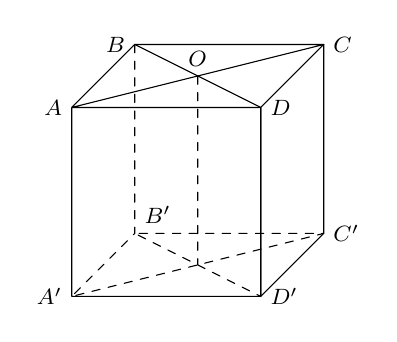
\begin{tikzpicture}[scale=0.4, font=\footnotesize, line join=round, line cap=round, >=stealth]
	\draw (0,0) node[left]{$A'$};
	\draw (2,2) node[above right]{$B'$};
	\draw (8,2) node[right]{$C'$};
	\draw (6,0) node[right]{$D'$};
	\draw (0,6) node[left]{$A$};
	\draw (2,8) node[left]{$B$};
	\draw (8,8) node[right]{$C$};
	\draw (6,6) node[right]{$D$};
	\draw (4,7) node[above]{$O$};
	\draw (0,0)--(0,6)--(6,6)--(6,0)--(0,0)(0,6)--(2,8)--(8,8)--(6,6)--(0,6)--(8,8);
	\draw (2,8)--(6,6)--(6,0) (8,8)--(8,2)--(6,0);
	\draw[dashed] (2,8)--(2,2)--(0,0)--(8,2)--(2,2)--(6,0) (4,7)--(4,1);
	\end{tikzpicture}
	}
	\item Ta có $(AA'D'D)\parallel (BB'C'C)$ suy ra \\
	$\mathrm{d}((AA'D'D),(BB'C'C))=\mathrm{d}(A,(BB'C'C))$.\\
	Do $AB\perp BB'$ và $AB\perp BC$, suy ra $AB\perp (BB'C'C)$.\\
	Vậy $\mathrm{d}((AA'D'D),(BB'C'C))=AB=a$.
	\end{enumerate}
	}
\end{bt}
\begin{bt}%[1C8B5-3]
	\immini
	{
	Cho hình chóp $S. A B C D$ có đáy $A B C D$ là hình vuông cạnh $a$, $S A \perp(A B C D)$. Chứng minh $C D \parallel (S A B)$ và tính khoảng cách giữa $C D$ và mặt phẳng $(S A B)$.
	}
	{
	\begin{tikzpicture}[scale=.6,font=\footnotesize, line join=round, line cap=round, >=stealth]
	\tkzDefPoints{0/0/A,5/0/D,-2/-2/B}
	\coordinate (C) at ($(B)+(D)-(A)$);
	\coordinate (S) at ($(A)+(0,4)$);
	\foreach \x/\g in {A/160,B/-100,C/-60,D/20,S/90} \fill[black](\x) circle (1.5pt) ($(\x)+(\g:3mm)$) node{$\x$};
	\draw (S)--(B)--(C)--(D)--(S)--(C);
	\draw[dashed] (B)--(A)--(D)
	(S)--(A);
	\end{tikzpicture}
	}
	\loigiai{
	Do $C D\parallel A B$, $A B \subset(S A B)$, $C D \not \subset(S A B)$ nên $C D \parallel (S A B)$.\\
	Vì $D \in C D$ nên $\mathrm{d}(C D,(S A B))=\mathrm{d}(D,(S A B))$.\\
	Do $S A \perp(A B C D)$, $D A \subset(A B C D)$ nên $S A \perp D A$.\\
	Vì $D A$ vuông góc với hai đường thẳng $A B$, $S A$ cắt nhau trong $(S A B)$ nên $D A \perp(S A B)$.\\
	Do đó $\mathrm{d}(D,(S A B))=D A=a$. Vậy $\mathrm{d}(C D,(S A B))=a$.
	}	
\end{bt}
\begin{bt}%[1C8B5-2]
	\immini
	{
	Cho hình hộp $A B C D. A' B' C' D'$ có tất cả các cạnh bằng $a$ và đáy là hình vuông. Hình chiếu của $A'$ trên mặt phẳng $(A B C D)$ là giao điểm $H$ của $A C$ và $B D$. Tính khoảng cách giữa hai mặt phẳng $(A B C D)$ và $\left(A' B' C' D'\right)$.
	}
	{\vspace*{-3mm}
	\begin{tikzpicture}[scale=.5,font=\footnotesize, line join=round, line cap=round, >=stealth]
	\tkzDefPoints{0/0/A,5/0/D,-2/-2/B}
	\coordinate (C) at ($(B)+(D)-(A)$);
	\coordinate (H) at ($(A)!.5!(C)$);
	\coordinate (A') at ($(H)+(0,5)$);
	\coordinate (B') at ($(B)+(A')-(A)$);
	\coordinate (C') at ($(C)+(A')-(A)$);
	\coordinate (D') at ($(D)+(A')-(A)$);
	\foreach \x/\g in {A/170,B/-120,C/-60,D/0,A'/90,B'/170,C'/-10,D'/60,H/-90} \fill[black](\x) circle (1.5pt) ($(\x)+(\g:4mm)$) node{$\x$};
	\draw (B')--(B)--(C)--(D)--(D')--(A')--(B')--(C')--(D')
	(C)--(C');
	\draw[dashed] (A)--(B)--(D)--(A)--(A')--(H)
	(A)--(C);
	\end{tikzpicture}
	}
	\loigiai{
	Vì $H$ là trung điểm của $A C$ nên $A H=\dfrac{A C}{2}=\dfrac{a \sqrt{2}}{2}$.\\
	Do $A' H \perp(A B C D)$ và $A H \subset(A B C D)$ nên $A' H \perp A H$.\\
	Xét tam giác $A A' H$ vuông tại $H$ có $A' H^2=A' A^2-A H^2=a^2-\left(\dfrac{a \sqrt{2}}{2}\right)^2=\dfrac{a^2}{2}$.\\
	Suy ra $A' H=\dfrac{a \sqrt{2}}{2}$.\\
	Vậy khoảng cách giữa hai mặt phẳng $(A B C D)$ và $\left(A' B' C' D'\right)$ bằng $A' H=\dfrac{a \sqrt{2}}{2}$.
	}
\end{bt}
\begin{bt}%[1H3K5]
	Hình chóp tứ giác đều $S. ABCD$ có cạnh đáy bằng $a$ và cạnh bên bằng $a \sqrt 2$.\begin{enumerate}
	\item Tính khoảng cách từ $S$ tới $(ABCD)$.
	\item Tính khoảng cách giữa đường thẳng $AB$ và mặt $(SCD)$.
	\end{enumerate}
	\loigiai{
	\immini{\begin{enumerate}
	\item Gọi $AC \cap BD =O$ suy ra $SO \perp (ABCD) $.\\
	Ta có $ \mathrm{d}(S; (ABCD))=SO=\sqrt{SA^2-OA^2}$. \\ Vậy $SO=\dfrac{a \sqrt 6}{2}$.
	\item Ta có $\mathrm{d}(AB; (SCD))=\mathrm{d}(A; (SCD))=2 \mathrm{d}(O; (SCD))=OH$. Tính được $OH=\dfrac{a \sqrt{42}}{14}$. 
	\end{enumerate}}{\begin{tikzpicture}[line join=round,scale=.7]
	\tkzDefPoints{0/0/A, -2/-2/B, 3/-2/C}
	\coordinate (D) at ($(A)+(C)-(B)$);
	\coordinate (O) at ($(A)!.5!(C)$);
	\coordinate (S) at ($(O)+(0,5)$);
	\tkzDrawPolygon(S,C,D)
	\tkzDefMidPoint(D,C)\tkzGetPoint{M}
	%	\tkzDrawAltitude[dashed](S,M)(O)\tkzGetPoint{H}	
	\coordinate (H) at ($(S)!(O)!(M)$);
	\tkzDrawSegments[dashed](S,A A,B A,D A,C B,D S,O O,M O,H)
	\tkzDrawSegments(S,B B,C S,M)
	\tkzLabelPoints[left](A,B)
	\tkzLabelPoints[below](O)
	\tkzLabelPoints[right](C,D,M)
	\tkzLabelPoints[above right](H)
	\tkzLabelPoints[above](S)
	\tkzMarkRightAngle(O,H,M)
	\end{tikzpicture}}
	}
\end{bt}
\begin{bt}%[1H3G5]
	Cho hình chóp $S. ABCD$ có đáy $ABCD$ là hình vuông cạnh $a$, $SA \perp (ABCD)$ và $SA=2a$.
	\begin{enumerate}
	\item Tính khoảng cách từ $A$ tới $(SBC)$ và khoảng cách từ $C$ tới $(SBD)$.
	\item $M, N$ lần lượt là trung điểm của $AB$ và $AD$. Tính khoảng cách từ $MN$ tới $(SBD)$.
	\item Mặt phẳng $(P)$ qua $BC$ cắt $SA, SD$ theo thứ tự tại $E, F$. Cho biết $AD$ cách $(P)$ một khoảng là $\dfrac{a\sqrt 2}{2}$, tính khoảng cách từ $S$ tới $(P)$ và diện tích tứ giác $BCFE$.
	\end{enumerate}
	\loigiai{
	\immini{\begin{enumerate}
	\item Hạ $AH \perp SB$ suy ra $AH \perp (SBC)$.
	Ta có $\mathrm{d}(A; (SBC))=AH=\dfrac{2a}{\sqrt{5}}$.
	\item $AC \cap BD=O$ suy ra $BD \perp (SAC)$. Hạ $AK \perp SO$ thì $AK \perp (SBD)$.
	Ta có $\mathrm{d}(C; (SBD))=\mathrm{d}(A; (SBD))=AK =\dfrac{2a}{3}$.
	\item Hạ $AQ \perp BE$ suy ra $AQ \perp (P)$. \\
	Ta có $\dfrac{1}{AQ^2}=\dfrac{1}{AB^2}+\dfrac{1}{AE^2}$ suy ra $AE=a$.\\
	Do đó $E$ là trung điểm của $SA$. $EF \parallel AD$ nên $F$ là trung điểm $SD$.\\
	$\mathrm{d}(S; (P))=\mathrm{d}(A; (P))=\mathrm{d}(AD; (P))=\dfrac{a \sqrt 2}{2}$.\\
	$BCFE$ là hình thang vuông tại $E,B$;
	$\mathcal{S}_{BCFE}=\dfrac{3a^2 \sqrt 2}{4}$.
	\end{enumerate}}{\begin{tikzpicture}[line join=round,scale=.8]
	\tkzDefPoints{0/0/A, -2/-2/B, 3/-2/C}
	\coordinate (D) at ($(A)+(C)-(B)$);
	\coordinate (S) at ($(A)+(0,5)$);
	%	\tkzDrawAltitude[dashed](S,B)(A)\tkzGetPoint{H}	
	\coordinate (H) at ($(S)!(A)!(B)$);
	\tkzInterLL(A,C)(B,D)\tkzGetPoint{O}
	\tkzDefMidPoint(S,A)\tkzGetPoint{E}
	\tkzDefMidPoint(D,S)\tkzGetPoint{F}
	%	\tkzDrawAltitude[dashed](S,O)(A)\tkzGetPoint{K}
	\coordinate (K) at ($(S)!(A)!(O)$);
	\tkzDrawSegments[dashed](S,A A,B A,D S,O A,C B,D B,E E,F A,K)
	\tkzDrawSegments(F,C)
	\tkzDrawPolygon(S,C,D)
	\tkzDrawSegments(S,B B,C)
	\tkzLabelPoints[left](A,B,E)
	\tkzLabelPoints[above left](K)
	\tkzLabelPoints[right](C,D,F)
	\tkzLabelPoints[below](O)
	\tkzLabelPoints[above left](H)
	\tkzLabelPoints[above](S)
	\tkzMarkRightAngle(D,A,S)
	\tkzMarkRightAngle(A,H,B)
	\tkzMarkRightAngle(A,K,S)
	\end{tikzpicture}}
	}
\end{bt}
\begin{bt}%[1H3G5]
	Cho hình chóp $S. ABCD$ có $SA=2a$ và vuông góc với mặt phẳng $(ABCD)$, đáy $ABCD$ là hình thang vuông tại $A$ và $B$, $AB=BC=a, AD=2a$.
	\begin{enumerate}
	\item Tính khoảng cách từ $A, B$ tới mặt phẳng $(SCD)$.
	\item Tính khoảng cách giữa đường thẳng $AD$ và mặt phẳng $(SBC)$.
	\item Tính diện tích của thiết diện của hình chóp $S. ABCD$ với mặt phẳng song song với $(SAD)$ và cách một khoảng bằng $\dfrac{a}{3}$.
	\end{enumerate}
	\loigiai{\begin{listEX}[2]
	\item $d(A; (SCD))=\dfrac{2a}{\sqrt 3}$; $d(B; (SCD))=\dfrac{a}{\sqrt 3}$.
	\item $d(AD; (SBC))=\dfrac{2a}{\sqrt 5}$.
	\item $\mathcal{S}_{EFGH}=\dfrac{4a^2}{3}$.
	\end{listEX}}
\end{bt}
%-----------------
\begin{dang}{Khoảng cách giữa hai đường thẳng chéo nhau}
\end{dang}
\begin{vd}%[1K7BP-4]
	Cho hình chóp $S.ABC$ có $SA\perp (ABC)$, $AB=a$, $\widehat{ABC}=60^\circ$.\\
	Xác định đường vuông góc chung và tính khoảng cách giữa hai đường thẳng $SA$ và $BC$.
	\loigiai{
	\immini{Gọi $H$ là hình chiếu của $A$ trên $BC$. Tam giác $ABH$ vuông tại $H$ và có $AB=a$, $\widehat{ABH}=60^\circ$ nên $BH=\dfrac{a}{2}$.\\
	Do $SA$ vuông góc với mặt phẳng $(ABC)$ nên $AH$ là đường vuông góc chung của $SA$ và $BC$ ($H$ thuộc tia $BC$ và $BH=\dfrac{a}{2}$).\\
	Khoảng cách giữa hai đường thẳng $SA$ và $BD$ là $\mathrm{d}(SA,BC)=AH=\dfrac{a\sqrt{3}}{2}$.}{\begin{tikzpicture}[scale=0.7,font=\footnotesize,line join = round, line cap = round, >= stealth]
	%\draw[opacity=0.3] (0,0) grid (6,6);
	\def\x{4} \def\y{2} \def\z{4}
	\def\g{-60}
	\coordinate (A) at (0,0);
	\coordinate (C) at ($(A)+(0:\x)$);
	\coordinate (B) at ($(A)+(\g:\y)$);
	\coordinate (S) at ($(A)+(90:\z)$);
	\coordinate (H) at ($(B)!.4!(C)$);
	\tkzMarkRightAngle(A,H,C)
	\begin{scope}
	\clip (C)--(B)--(A);
	\draw (B) circle (0.3);
	\draw ($(B)+(60:0.6)$)node[rotate=0]{$60^\circ$};
	\end{scope}
	\draw (S)--(A)--(B)--(C)--(S)--(B);
	\draw[dashed] (C)--(A)--(H);
	\foreach \p/\g in {S/100,A/180,B/-90,H/-80,C/0} \draw[fill] (\p) circle(.5pt)
	node [shift={(\g:.3)}] {$\p$}
	;
	\end{tikzpicture}}
	}
\end{vd}
\begin{vd}%[1K7KP-4]
	\textbf{Luyện tập 3.} 
	Cho hình chóp $S.ABCD$ có đáy là hình vuông cạnh $a$, $SA\perp (ABCD)$, $SA=a\sqrt{2}$.
	\begin{enumerate}
	\item Tính khoảng cách từ $A$ đến $SC$.
	\item Chứng minh rằng $BD\perp (SAC)$.
	\item Xác định đường vuông góc chung và tính khoảng cách giữa $BD$ và $SC$.
	\end{enumerate}
	\loigiai{
	\immini{
	\begin{enumerate}
	\item Tính khoảng cách từ $A$ đến $SC$.\\
	Gọi $H$ là trung điểm $SC$. Ta có $AC=SA=a\sqrt{2}$, suy ra tam giác $SAC$ vuông cân tại $A$ nên $AH\perp SC$.\\
	Vậy $\mathrm{d}(A,SC)=AH=a$.
	\item Chứng minh rằng $BD\perp (SAC)$.\\
	Do $\heva{&BD\perp AC\\&BD\perp SA}$ $\Rightarrow BD\perp (SHC)$.
	\item Xác định đường vuông góc chung và tính khoảng cách giữa $BD$ và $SC$.\\
	Gọi $O=AC\cap BD$. Kẻ $OK\perp SC$ tại $K$.\\
	Do $BD\perp (SAC)$ nên $OK\perp BD$.\\
	Vậy $OK$ là đường vuông góc chung giữa $BD$ và $SC$.\\
	Xét $\triangle SAC\backsim \triangle OKC\Rightarrow \dfrac{OK}{SA}=\dfrac{OC}{SC}$ $\Rightarrow OK=\dfrac{OC\cdot SA}{SC}=\dfrac{a\sqrt{2}\cdot a\sqrt{2}}{2\cdot 2a}=\dfrac{a}{2}$.
	\end{enumerate}
	}{
	\begin{tikzpicture}[scale=1,font=\footnotesize,line join = round, line cap = round, >= stealth]
	%\draw[opacity=0.3] (0,0) grid (6,6);
	\def\x{4} \def\y{2} \def\z{2.5}
	\def\g{-120}
	\coordinate (A) at (0,0);
	\coordinate (D) at ($(A)+(0:\x)$);
	\coordinate (B) at ($(A)+(\g:\y)$);
	\coordinate (C) at ($(B)+(D)-(A)$);
	\coordinate (S) at ($(A)+(90:\z)$);
	\coordinate (O) at ($(B)!1/2!(D)$);
	\coordinate (H) at ($(S)!1/2!(C)$);
	\coordinate (K) at ($(H)!1/2!(C)$);
	\draw (S)--(B)--(C)--(D)--(S)--(C);
	\draw[dashed] (S)--(A)--(C) (B)--(D)
	(B)--(A)--(D) (A)--(H) (O)--(K)
	;
	\tkzMarkRightAngles(A,H,S O,K,C)
	\foreach \p/\g in {S/100,A/180,B/-90,C/-70,D/0,O/-90,H/60,K/20} \draw[fill] (\p) circle(.5pt)
	node [shift={(\g:.3)}] {$\p$}
	;
	\end{tikzpicture}
	}
	}
\end{vd}
\begin{vd}%[1H3K5]
	Cho hình chóp $S.ABCD$ có đáy là hình vuông $ABCD$ cạnh $a$, có cạnh $SA = h$ và vuông góc với mặt phẳng $(ABCD)$. Dựng và tính độ dài đoạn vuông góc chung của hai đường thẳng chéo nhau:
	\begin{multicols}{3}
	\begin{enumerate}[a)]
	\item $SB$ và $CD$.
	\item $SC$ và $BD$.
	\item $SC$ và $AB$.
	\end{enumerate}
	\end{multicols}
	\loigiai{
	\begin{center}
	\begin{tikzpicture}[line join=round,scale=0.7]
	\tkzDefPoints{0/0/A,-3/-3/B,3/-3/C,6/0/D,0/5/S}
	\tkzDefPointBy[homothety = center S ratio 0.6](D) \tkzGetPoint{K}
	\tkzDefPointBy[homothety = center S ratio 0.6](C) \tkzGetPoint{E}
	\tkzDefPointBy[homothety = center S ratio 0.7](C) \tkzGetPoint{H}	
	\tkzDefPointBy[translation = from K to A](E) \tkzGetPoint{F}
	\tkzInterLL(A,C)(B,D) \tkzGetPoint{O}
	\tkzDrawSegments(B,C C,D S,B S,C S,D E,K)
	\tkzDrawSegments[dashed](A,B A,D S,A A,K E,F A,C B,D O,H)
	\tkzMarkRightAngles[size=.3](S,A,B S,A,D B,A,D S,K,A F,E,C E,F,B O,H,C B,O,H)
	\tkzDrawPoints(H,E,F,K,O) 
	\tkzLabelPoints(C)
	\tkzLabelPoints[above](S)
	\tkzLabelPoints[below](O) 	
	\tkzLabelPoints[right](D,E,H,K)
	\tkzLabelPoints[left](F)
	\tkzLabelPoints[below left](B)
	\tkzLabelPoints[above left](A)
	\end{tikzpicture}
	\end{center}
	\begin{enumerate}[a)]
	\item Ta có: $\heva{&BC \perp SA\\ &BC \perp AB}$ $\Rightarrow BC \perp (SAB) \Rightarrow BC \perp SB$.\\
	Mặt khác $BC \perp CD$. Vậy $BC$ là đoạn vuông góc chung của $SB$ và $CD$.\\
	Suy ra $d(SB, CD) = BC = a$.
	\item Gọi $O$ là giao điểm của $AC$ và $BD$. Ta có: $\heva{&BD \perp SA\\ &BD \perp AC}$ $\Rightarrow BD \perp (SAC)$ tại $O$.\\
	Trong mặt phẳng $(SAC)$, kẻ $OH \perp SC$ tại $H$, ta có $OH \perp SC$ và $OH \perp BD$ (vì $BD \perp (SAC)$).\\
	Vậy $OH$ là đoạn vuông góc chung của $BD$ và $SC$.\\
	Ta có $\dfrac{OH}{OC} = \dfrac{SA}{SC} = \sin \widehat{ACS}$ $\Rightarrow OH = \dfrac{OC.SA}{SC} = \dfrac{a\sqrt{2}}{2}\cdot \dfrac{h}{\sqrt{h^2 + 2a^2}}$.\\
	Vậy $d(SC, BD) = OH = \dfrac{ah\sqrt{2}}{2\sqrt{h^2 + 2a^2}}$.
	\item Ta có $AB \parallel CD$ $\Rightarrow AB \parallel (SCD)$.\\
	Ta có: $\heva{&CD \perp SA\\ &CD \perp AD}$ $\Rightarrow CD \perp (SAD)$ $\Rightarrow (SCD) \perp (SAD)$ theo giao tuyến $SD$.\\
	Trong mặt phẳng $(SAD)$, kẻ $AK \perp SD$ tại $K$, ta có: $AK \perp (SCD)$ $\Rightarrow AK \perp SC$.\\
	Trong mặt phẳng $(SCD)$, kẻ $KE \parallel CD$ $(E \in SC)$.\\
	Trong mặt phẳng $(AB, KE)$, kẻ $EF \parallel AK$ $(F \in AB)$ $\Rightarrow EF \perp SC$.\\
	Lại có $AB \parallel CD$ và $CD \perp (SAD)$ $\Rightarrow AB \perp (SAD)$ $\Rightarrow AB \perp AK$ $\Rightarrow AB \perp EF$.\\
	Do đó $EF$ là đoạn vuông góc chung của $SC$ và $AB$.\\
	Ta có $EF = AK = \dfrac{SA.AD}{SD} = \dfrac{ah}{\sqrt{a^2 + h^2}}$.\\
	Vậy $d(SC, AB) = \dfrac{ah}{\sqrt{a^2 + h^2}}$.
	\end{enumerate}
	}
\end{vd}
\begin{vd}%[1H3K5]
	Cho tứ diện $OABC$ có $OA$, $OB$, $OC$ vuông góc với nhau đôi một và $OA = OB = OC = a$. Gọi $I$ là trung điểm của $BC$. Hãy dựng và tính độ dài đoạn vuông góc chung của các cặp đường thẳng chéo nhau:
	\begin{multicols}{2}
	\begin{enumerate}[a)]
	\item $OA$ và $BC$.
	\item $AI$ và $OC$.
	\end{enumerate}
	\end{multicols}
	\loigiai{
	\begin{center}
	\begin{tikzpicture}[line join=round,scale=0.85]
	\tkzDefPoints{0/0/O,0/5/A,5/-3/B,7/0/C}
	\tkzDefMidPoint(B,C) \tkzGetPoint{I}
	\tkzDefMidPoint(O,B) \tkzGetPoint{K}
	\tkzDefPointBy[homothety = center A ratio 0.6](K) \tkzGetPoint{H}
	\tkzDefPointBy[homothety = center A ratio 0.6](I) \tkzGetPoint{E}
	\tkzDefPointBy[translation = from H to O](E) \tkzGetPoint{F}
	\tkzDrawSegments(O,A O,B B,C A,K A,B A,I A,C O,H)
	\tkzDrawSegments[dashed](O,C K,I H,E E,F O,I)
	\tkzMarkRightAngles[size=.3](A,O,B A,O,C B,O,C O,H,K F,E,I E,F,C I,K,B)
	\tkzDrawPoints(I,K,H,E,F)
	\tkzLabelPoints[above](A)
	\tkzLabelPoints[below](B) 	
	\tkzLabelPoints[right](E,I,C)
	\tkzLabelPoints[left](O,H)
	\tkzLabelPoints[below left](K)
	\tkzLabelPoints[](F)
	\end{tikzpicture}
	\end{center}
	\begin{enumerate}[a)]
	\item Ta có $\heva{&OA \perp OI\\ &BC \perp OI}$ $\Rightarrow OI$ là đoạn vuông góc chung của $OA$ và $BC$.\\
	Tam giác $OBC$ vuông cân tại $O$ nên $OI = \dfrac{BC}{2} = \dfrac{a\sqrt{2}}{2}$.\\
	Vậy $d(OA, BC) = \dfrac{a\sqrt{2}}{2}$.
	\item Gọi $K$ là trung điểm của $OB$, ta có $IK \parallel OC$ $\Rightarrow OC \parallel (AIK)$.\\
	Ta có $\heva{&IK \perp OB\\ &IK \perp OA}$ $\Rightarrow IK \perp (OAB)$ $\Rightarrow (AIK) \perp (OAB)$ theo giao tuyến $AK$.\\
	Trong mặt phẳng $(OAB)$, kẻ $OH \perp AK$ tại $H$, ta có: $OH \perp (AIK)$ $\Rightarrow OH \perp AI$.\\
	Trong mặt phẳng $(AIK)$, kẻ $HE \parallel IK$ $(E \in SI)$.\\
	Trong mặt phẳng $(HE, OC)$, kẻ $EF \parallel OH$ $(F \in OC)$ $\Rightarrow EF \perp AI$.\\
	Lại có $OC \perp (OAB) \Rightarrow OC \perp AH \Rightarrow OC \perp EF$.\\
	Do đó $EF$ là đoạn vuông góc chung của $OC$ và $AI$.\\
	Trong tam giác vuông $OAK$ ta có: $\dfrac{1}{OH^2} = \dfrac{1}{OA^2} + \dfrac{1}{OK^2} = \dfrac{1}{a^2} + \dfrac{4}{a^2} = \dfrac{5}{a^2}$.\\
	Suy ra $EF = OH = \dfrac{a\sqrt{5}}{5}$.\\
	Vậy $d(AI, OC) = \dfrac{a\sqrt{5}}{5}$.
	\end{enumerate}
	}
\end{vd}
\begin{vd}%[1H3K5]
	Cho hình lăng trụ đứng $ABC.A'B'C'$ có đáy $ABC$ là tam giác vuông tại $A$ với $AB = a$, $AC = 2a$; cạnh bên $AA' = 2a$. Hãy dựng và tính độ dài đoạn vuông góc chung của hai đường thẳng $BC'$ và $AA'$.
	\loigiai{
	\begin{center}
	\begin{tikzpicture}[line join=round,scale=0.6]
	\tkzDefPoints{0/0/A,2/-3/B,6/0/C,0/7/A'}
	\tkzDefPointBy[translation = from A to A'](B) \tkzGetPoint{B'}
	\tkzDefPointBy[translation = from A to A'](C) \tkzGetPoint{C'}
	\tkzDefPointBy[homothety = center B' ratio 0.4](C') \tkzGetPoint{H}
	\tkzDefPointBy[homothety = center B ratio 0.4](C') \tkzGetPoint{F}
	\tkzDefPointBy[translation = from H to F](A') \tkzGetPoint{E}
	\tkzDrawSegments(A,B B,C A,A' A',B' B',C' A',C' A',H H,F B,C' B,B' C,C')
	\tkzDrawSegments[dashed](A,C E,F)
	\tkzMarkRightAngles[size=.3](B',A',C' A',H,B' A',E,F E,F,B A,A',B')
	\tkzDrawPoints(H,E,F)
	\tkzLabelPoints[above left](A')
	\tkzLabelPoints[above right](C')
	\tkzLabelPoints[below](B) 	
	\tkzLabelPoints[right](C,F)
	\tkzLabelPoints[left](A,E)
	\tkzLabelPoints[below left](B') 
	\tkzLabelPoints(H)	
	\end{tikzpicture}
	\end{center}
	Ta có $AA' \parallel BB'$ $\Rightarrow AA' \parallel (BB'C'C)$.\\
	Vì $(A'B'C') \perp (BB'C'C)$ theo giao tuyến $B'C'$ nên trong mặt phẳng $(A'B'C')$, kẻ $A'H \perp B'C'$ tại $H$, ta có: $A'H \perp (BB'C'C)$ $\Rightarrow A'H \perp BC'$.\\
	Trong mặt phẳng $(BB'C'C)$, kẻ $HF \parallel AA'$ $(F \in BC')$.
	Trong mặt phẳng $(HF, AA')$, kẻ $FE \parallel A'H$ $(E \in AA')$ $\Rightarrow FE \perp BC'$.\\
	Ta có $AA' \perp (A'B'C') \Rightarrow AA' \perp A'H \Rightarrow AA' \perp FE$.\\
	Do đó $EF$ là đoạn vuông góc chung của $AA'$ và $BC'$.\\
	Trong tam giác vuông $A'B'C'$ ta có: $\dfrac{1}{A'H^2} = \dfrac{1}{A'B'^2} + \dfrac{1}{A'C'^2} = \dfrac{1}{a^2} + \dfrac{1}{4a^2} = \dfrac{5}{4a^2}$.\\
	Suy ra $EF = A'H = \dfrac{2a\sqrt{5}}{5}$.\\
	Vậy $d(AA', BC') = \dfrac{2a\sqrt{5}}{5}$.
	}
\end{vd}
\begin{vd}%[1H3K5]
	Cho hình chóp $S.ABC$ có đáy là tam giác đều cạnh $a$. $SA=2a$ và vuông góc với mặt đáy. Tính khoảng cách giữa hai đường thẳng $SB$ và $AC$.
	\loigiai{
	\begin{center}
	\begin{tikzpicture}[line join=round,scale=0.6]
	\tkzDefPoints{0/0/A,2/-3/B,7/0/C,0/5/S,-5/-3/D} 	
	\tkzDefMidPoint(B,D) \tkzGetPoint{I}
	\tkzDefPointBy[homothety = center S ratio 0.4](I) \tkzGetPoint{H}
	\tkzDrawSegments(S,B S,C S,D S,I B,C B,D)
	\tkzDrawSegments[dashed](S,A A,B A,C A,D A,I A,H)
	\tkzMarkRightAngles[size=.3](C,A,S S,A,I I,H,A B,I,A)
	\tkzDrawPoints(I,H) 
	\tkzLabelPoints[below right](B)
	\tkzLabelPoints[above](S) 	
	\tkzLabelPoints[right](C)
	\tkzLabelPoints[left](A,D,H)
	\tkzLabelPoints[below](I)
	\end{tikzpicture}
	\end{center}
	Trong mặt phẳng $(ABC)$, dựng hình thoi $ACBD$, ta có: $BD \parallel AC \Rightarrow AC \parallel (SBD)$.\\
	$\Rightarrow d(AC,SB)=d(AC,(SBD))=d(A,(SBD))$.\\
	Gọi $I$ là trung điểm của $BD$, ta có: $BD \perp AI$ và $BD \perp SA$ $\Rightarrow BD \perp (SAI)$.\\
	$\Rightarrow (SBD) \perp (SAI)$ theo giao tuyến $SI$.\\
	Trong mặt phẳng $(SAI)$, kẻ $AH \perp SI$ tại $H$, ta có: $AH \perp (SBD)$ $\Rightarrow AH=d(A,(SBD))$.\\
	Tam giác $SAI$ vuông tại $A$ có đường cao $AH$.\\
	$\Rightarrow \dfrac{1}{AH^2}=\dfrac{1}{SA^2}+\dfrac{1}{AI^2}=\dfrac{1}{4a^2}+\dfrac{4}{3a^2}=\dfrac{19}{12a^2}$.\\
	$\Rightarrow AH^2=\dfrac{12a^2}{19}$ hay $AH=\dfrac{2a\sqrt{57}}{19}$.\\
	Vậy $d(SB, AC) = \dfrac{2a\sqrt{57}}{19}$.
	}
\end{vd}
\begin{vd}%[1H3G5]
	Cho hình chóp $S.ABCD$ có đáy là hình vuông cạnh bằng $a$, $SA$ vuông góc với đáy và $SA = a$. $M$ là trung điểm của $SB$. Tính khoảng cách giữa các đường thẳng:
	\begin{multicols}{3}
	\begin{enumerate}[a)]
	\item $SC$ và $BD$.
	\item $AC$ và $SD$.
	\item $SD$ và $AM$.
	\end{enumerate}
	\end{multicols}
	\loigiai{
	\begin{center}
	\begin{tikzpicture}[line join=round,scale=0.7]
	\tkzDefPoints{0/0/A,-3/-3/D,3/-3/C,6/0/B,0/5/S}
	\tkzDefMidPoint(S,B) \tkzGetPoint{M}
	\tkzInterLL(A,C)(B,D) \tkzGetPoint{O}
	\tkzDefPointBy[translation = from C to D](A) \tkzGetPoint{E}	
	\tkzDefPointBy[translation = from O to D](A) \tkzGetPoint{I}
	\tkzDefPointBy[homothety = center S ratio 0.7](C) \tkzGetPoint{H}
	\tkzDefPointBy[homothety = center S ratio 0.6](I) \tkzGetPoint{K}
	\tkzDrawSegments(S,E S,D S,C S,B C,D B,C M,C D,E S,I)
	\tkzDrawSegments[dashed](S,A A,D A,B A,K A,E A,M O,M O,H A,C B,D A,I)
	\tkzMarkRightAngles[size=.3](S,A,B S,A,D B,A,D A,I,D A,K,I O,H,C D,O,H)
	\tkzDrawPoints(O,M,H,K) 
	\tkzLabelPoints(C)
	\tkzLabelPoints[above](S)
	\tkzLabelPoints[below](O) 	
	\tkzLabelPoints[right](H,B)
	\tkzLabelPoints[left](E,K,I)
	\tkzLabelPoints[below left](D)
	\tkzLabelPoints[above left](A)
	\tkzLabelPoints[above right](M)
	\end{tikzpicture}
	\end{center}
	\begin{enumerate}[a)]
	\item Gọi $O$ là giao điểm của $AC$ và $BD$. Ta có: $\heva{&BD \perp SA\\ &BD \perp AC}$ $\Rightarrow BD \perp (SAC)$ tại $O$.\\
	Trong mặt phẳng $(SAC)$, kẻ $OH \perp SC$ tại $H$, ta có $OH \perp SC$ và $OH \perp BD$ (vì $BD \perp (SAC)$).\\
	Vậy $OH$ là đoạn vuông góc chung của $BD$ và $SC$.\\
	Ta có $\dfrac{OH}{OC} = \dfrac{SA}{SC} = \sin \widehat{ACS}$ $\Rightarrow OH = \dfrac{OC.SA}{SC} = \dfrac{\dfrac{a\sqrt{2}}{2}\cdot a}{a\sqrt{3}} = \dfrac{a\sqrt{6}}{6}$.\\
	Vậy $d(SC, BD) = OH = \dfrac{a\sqrt{6}}{6}$.
	\item Dựng hình bình hành $ACDE$, ta có: $AC \parallel DE$ $\Rightarrow AC \parallel (SDE)$.\\
	$\Rightarrow d(AC, SD) = d(AC, (SDE)) = d(A, (SDE))$.\\
	Trong mặt phẳng $(ABCD)$, kẻ $AI \perp DE$ tại $I$, ta có $\heva{&DE \perp AI\\ &DE \perp SA}$ $\Rightarrow DE \perp (SAI)$.\\
	$\Rightarrow (SDE) \perp (SAI)$ theo giao tuyến $SI$.\\
	Trong mặt phẳng $(SAI)$, kẻ $AK \perp SI$ tại $K$, ta có: $AK \perp (SDE)$ $\Rightarrow AK = d(A, (SDE))$.\\
	Ta có $AIDO$ là hình bình hành nên $AI = OD = \dfrac{a\sqrt{2}}{2}$.\\
	Trong tam giác vuông $SAI$ ta có: $\dfrac{1}{AK^2} = \dfrac{1}{AI^2} + \dfrac{1}{SA^2} = \dfrac{2}{a^2} + \dfrac{1}{a^2} = \dfrac{3}{a^2}$.\\
	Suy ra $AK = \dfrac{a\sqrt{3}}{3}$.\\
	Vậy $d(AC, SD) = d(A, (SDE)) = AK = \dfrac{a\sqrt{3}}{3}$.
	\item Ta có $OM \parallel SD$ và $AC \parallel DE$ nên $(AMC) \parallel (SDE)$.\\
	Suy ra $d(SD, AM) = d((AMC), (SDE)) = d(A, (SDE)) = AK = \dfrac{a\sqrt{3}}{3}$.
	\end{enumerate}
	}
\end{vd}
\subsubsection{Bài tập áp dụng}
\begin{vd}%[1T8B4-4]
	Cho hình chóp $S.ABCD$ có đáy là hình vuông $ABCD$ cạnh $a$, cạnh $SA=a$ và vuông góc với mặt phẳng $(ABCD)$. Tính khoảng cách giữa hai đường thẳng:
	\begin{enumerate}
	\item $SB$ và $CD$.
	\item $AB$ và $SC$.
	\end{enumerate}
	\loigiai{
	\begin{enumerate}
	\item Ta có $BC\perp SA$ và $BC\perp AB$, suy ra $BC\perp SB$.\\
	Mặt khác $BC\perp CD$, suy ra $BC$ là đoạn vuông góc chung của hai đường thẳng $SB$ và $CD$. Ta có $\mathrm{d}(SB,CD)=BC=a$.
	\item 
	\immini
	{\textbf{Cách 1.} Ta có $AB\perp(SAD)$ và $SD$ là hình chiếu vuông góc của $SC$ lên $(SAD)$.\\
	Vẽ $AK\perp SD$, $KE\parallel AB$, $EF\parallel AK$.\\
	Ta có $AB\perp AK$, $AK\perp SD$, suy ra $AK\perp SC$. Do $EF\parallel AK$, suy ra ta cũng có $EF\perp AB$ và $EF$ cắt $AB$ tại $F$, $EF\perp SC$ và $EF$ cắt $SC$ tại $E$.\\
	Các kết quả trên chứng tỏ $EF$ là đoạn vuông góc chung của $AB$ và $SC$.
	}
	{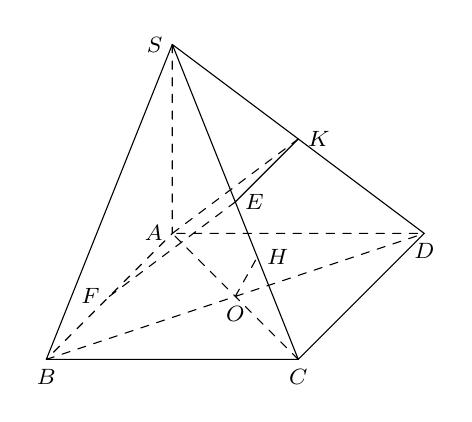
\begin{tikzpicture}[scale=0.4, font=\footnotesize, line join=round, line cap=round, >=stealth]
	\draw (4,4) node[left]{$A$};
	\draw (0,0) node[below]{$B$};
	\draw (8,0) node[below]{$C$};
	\draw (12,4) node[below]{$D$};
	\draw (2,2) node[left]{$F$};
	\draw (6,5) node[right]{$E$};
	\draw (8,7) node[right]{$K$};
	\draw (6,2) node[below]{$O$};
	\draw (4,10) node[left]{$S$};
	\draw (6.7,3.25) node[right]{$H$};
	\coordinate (A) at (4,4);
	\coordinate (B) at (0,0);
	\coordinate (C) at (8,0);
	\coordinate (D) at (12,4);
	\coordinate (F) at (2,2);
	\coordinate (E) at (6,5);
	\coordinate (K) at (8,7);
	\coordinate (O) at (6,2);
	\coordinate (S) at (4,10);
	\coordinate (H) at (6.7,3.25);
	\draw (S)--(B)--(C)--(D)--(S)--(C) (E)--(K);
	\draw[dashed] (S)--(A)--(B) (C)--(A)--(D) (A)--(K) (F)--(E) (O)--(H)(B)--(D);
	\tkzMarkRightAngle(S,K,A);
	\tkzMarkRightAngle(O,H,C);
	\tkzMarkRightAngle(C,E,F);
	\end{tikzpicture}
	}
	Trong tam giác $SAD$ vuông cân tại $A$ có $AK=\dfrac{SD}{2}=\dfrac{a\sqrt{2}}{2}$.\\
	Vậy $\mathrm{d}(AB,SC)=EF=AK=\dfrac{a\sqrt{2}}{2}$.\\
	\textbf{Cách 2.} Ta có mặt phẳng $(SCD)$ chứa $SC$ và song song với $AB$, suy ra
	\[\mathrm{d}(AB,SC)=\mathrm{d}(AB,(SCD))=\mathrm{d}(A,(SCD))=\dfrac{a\sqrt{2}}{2}.\]
	\end{enumerate}
	}
\end{vd}
\begin{vd}%[1C8B5-5]
	\immini
	{
	Cho lăng trụ $A B C D. A' B' C' D'$ có đáy $A B C D$ là hình vuông cạnh $2 a$, $O$ là giao điểm của $A C$ và $B D$, $A A'=a$, $A A'$ vuông góc với mặt phẳng chứa đáy. Tính
	\begin{enumerate}
	\item $\mathrm{d}\left(A C, A' B'\right)$;
	\item $\mathrm{d}\left(C C', B D\right)$.
	\end{enumerate}
	}
	{
	\begin{tikzpicture}[scale=.7,font=\footnotesize, line join=round, line cap=round, >=stealth]
	\tkzDefPoints{0/0/A,5/0/D,-2/-2/B}
	\coordinate (C) at ($(B)+(D)-(A)$);
	\coordinate (O) at ($(A)!.5!(C)$);
	\coordinate (A') at ($(A)+(0,4)$);
	\coordinate (B') at ($(B)+(A')-(A)$);
	\coordinate (C') at ($(C)+(A')-(A)$);
	\coordinate (D') at ($(D)+(A')-(A)$);
	\foreach \x/\g in {A/170,B/-120,C/-60,D/0,A'/90,B'/170,C'/-10,D'/60,O/-90} \fill[black](\x) circle (1.5pt) ($(\x)+(\g:4mm)$) node{$\x$};
	\draw (B')--(B)--(C)--(D)--(D')--(A')--(B')--(C')--(D')
	(C)--(C');
	\draw[dashed] (A)--(B)--(D)--(A)--(A')
	(A)--(C);
	\end{tikzpicture}
	}
	\loigiai{
	\begin{enumerate}
	\item Vì $A A'$ vuông góc với cả hai mặt phẳng $(A B C D)$ và $\left(A' B' C' D'\right)$ nên $A A' \perp A C$, $A A' \perp A' B'$.\\
	Suy ra đoạn thẳng $A A'$ là đoạn vuông góc chung của $A C$ và $A' B'$. Vậy $\mathrm{d}\left(A C, A' B'\right)=A A'=a$.
	\item Vì $C C'$ vuông góc với $(A B C D)$ nên $C C' \perp O C$. Do đáy $A B C D$ là hình vuông có $O$ là giao điểm của $A C$ và $B D$ nên $B D \perp O C$. Suy ra đoạn thẳng $O C$ là đoạn vuông góc chung của $C C'$ và $B D$. Vậy $\mathrm{d}\left(C C', B D\right)=O C=a \sqrt{2}$.
	\end{enumerate}
	}
\end{vd}
\begin{vd}%[1H3K5]
	Cho hình chóp $S.ABCD$ có đáy là hình vuông cạnh bằng $a$; $SA$ vuông góc với đáy và $SA = a$; $M$, $N$ lần lượt là trung điểm của $AB$ và $SC$. Chứng minh rằng $MN$ là đoạn vuông góc chung của $AB$ và $SC$. Tính khoảng cách giữa $AB$ và $SC$.
	\loigiai{
	\begin{center}
	\begin{tikzpicture}[line join=round,scale=0.7]
	\tkzDefPoints{0/0/A,-3/-3/B,3/-3/C,6/0/D,0/5/S}
	\tkzDefMidPoint(A,B) \tkzGetPoint{M}
	\tkzDefMidPoint(S,C) \tkzGetPoint{N}
	\tkzDefMidPoint(A,C) \tkzGetPoint{O}
	\tkzDrawSegments(S,B S,C S,D B,C C,D)
	\tkzDrawSegments[dashed](S,A A,B A,D A,C M,N N,O O,M S,M)
	\tkzMarkRightAngles[size=.3](S,A,B S,A,D B,A,D M,O,N N,O,C)
	\tkzDrawPoints(O,M,N) 
	\tkzLabelPoints[above](S)
	\tkzLabelPoints[below](O)
	\tkzLabelPoints[left](M)
	\tkzLabelPoints[above left](A)
	\tkzLabelPoints[right](D,N) 	
	\tkzLabelPoints[below left](B)
	\tkzLabelPoints(C)
	\end{tikzpicture}
	\end{center}
	Gọi $O$ là tâm của hình vuông $ABCD$, ta có $ON$ là đường trung bình của tam giác $SAC$ $\Rightarrow ON \parallel SA$ $\Rightarrow ON \perp (ABCD)$.\\
	Suy ra $MO$ là hình chiếu của $MN$ trên mặt phẳng $(ABCD)$.\\
	Mà $MO \perp AB$ nên $MN \perp AB$ (định lí ba đường vuông góc.\\
	Tam giác $MON$ vuông tại $O$ $\Rightarrow MN^2 = MO^2 + ON^2 = \dfrac{a^2}{4} + \dfrac{a^2}{4} = \dfrac{2a^2}{4}$.\\
	Tam giác $SAM$ vuông tại $M$ $\Rightarrow SM^2 = SA^2 + AM^2 = a^2 + \dfrac{a^2}{4} = \dfrac{5a^2}{4}$.\\
	Ta có $SN^2 = \left(\dfrac{SC}{2}\right)^2 = \dfrac{SA^2 + AC^2}{4} = \dfrac{a^2 + 2a^2}{4} = \dfrac{3a^2}{4}$.\\
	Suy ra $SM^2 = SN^2 + MN^2$ hay tam giác $SMN$ vuông tại $N$ $\Rightarrow MN \perp SC$.\\
	Do đó $MN$ là đoạn vuông góc chung của $AB$ và $SC$.\\
	Vậy $d(AB, SC) = MN = \dfrac{a\sqrt{2}}{2}$.
	}
\end{vd}
\begin{vd}%[1H3K5]
	Cho hình lập phương $ABCD.A'B'C'D'$. Xác định đường vuông góc chung của hai đường thẳng $BD$ và $B'C$.
	\loigiai{
	\begin{center}
	\begin{tikzpicture}[line join=round,scale=0.7]
	\tkzDefPoints{0/0/A, 6/0/B, -2/-2.5/D, 4/-2.5/C, 0/-6/A'}
	\tkzDefPointBy[translation = from A to A'](B) \tkzGetPoint{B'}
	\tkzDefPointBy[translation = from A to A'](C) \tkzGetPoint{C'}	
	\tkzDefPointBy[translation = from A to A'](D) \tkzGetPoint{D'}
	\tkzDefMidPoint(B,C) \tkzGetPoint{I}
	\tkzInterLL(A,I)(B,D) \tkzGetPoint{M}
	\tkzInterLL(B',C)(C',I) \tkzGetPoint{N}
	\tkzDrawSegments(A,B B,C C,D D,A D,D' C,C' B,B' D',C' B',C' B,D A,I B',C C',I)
	\tkzDrawSegments[dashed](A,A' A,C' A',D' A',B' M,N)
	\tkzDrawPoints(I,M,N)
	\tkzLabelPoints[above left](A)
	\tkzLabelPoints[left](A',D)
	\tkzLabelPoints[right](B',N,I) 
	\tkzLabelPoints[below left](C,D')
	\tkzLabelPoints[above right](B)
	\tkzLabelPoints(C')
	\tkzLabelPoints[above](M)
	\end{tikzpicture}
	\end{center}
	Ta có $BD \perp (ACC'A")$ $\Rightarrow BD \perp AC'$.\\
	Lại có $B'C \perp (ABC')$ $\Rightarrow B'C \perp AC'$.\\
	Vậy ta có đường thẳng $AC'$ vuông góc với cả hai đường thẳng $B'C$ và $BD$.\\
	Lấy điểm $I$ thuộc $BC$. Gọi $M$ là giao điểm của $AI$ và $BD$; $N$ là giao điểm của $IC'$ và $B'C$.\\
	Ta cần tìm vị trí của $I$ để $MN \parallel AC'$.\\
	Ta có $MN \parallel AC'$ $\Leftrightarrow \dfrac{IM}{MA} = \dfrac{IN}{NC'} \Leftrightarrow \dfrac{IB}{AD} = \dfrac{IC}{B'C'} \Leftrightarrow IB = IC$.\\
	Vậy khi $I$ là trung điểm của $BC$ thì $MN$ là đoạn vuông góc chung của hai đường thẳng $BD$ và $B'C$ với $M$ là giao điểm của $AI$ và $BD$; $N$ là giao điểm của $IC'$ và $B'C$.
	}
\end{vd}
\begin{vd}%[1H3K5]
	Cho hình chóp $S. ABCD$ có đáy $ABCD$ là hình vuông tâm $O$ cạnh $a$, $SO$ vuông góc với mặt phẳng đáy $\left(ABCD\right)$ và $SO=a$. Tính Khoảng cách giữa hai đường thẳng $SC$ và $AB$.
	\loigiai{
	\begin{center}
	\begin{tikzpicture}[line join=round,scale=0.85]
	\tkzDefPoints{0/0/O, -4/-1/A, 1/-1/D, 0/6/S}
	\tkzDefPointBy[symmetry = center O](D) 	\tkzGetPoint{B}
	\tkzDefPointBy[symmetry = center O](A) 	\tkzGetPoint{C}	
	\tkzDefMidPoint(C,D) \tkzGetPoint{I}
	\tkzDefPointBy[homothety = center S ratio 0.7](I) \tkzGetPoint{H}
	\tkzDrawSegments[dashed](A,C B,D S,O S,B C,B A,B O,I O,H)
	\tkzDrawSegments(S,A S,C S,D C,D A,D S,I)
	\tkzDrawPoints(O,H,I) 
	\tkzLabelPoints[below](O)
	\tkzLabelPoints[below left](A)
	\tkzLabelPoints[above](S)
	\tkzLabelPoints[right](C,H)
	\tkzLabelPoints[above left](B)
	\tkzLabelPoints(I,D)
	\tkzMarkRightAngles[size=.3](O,H,I S,O,I O,I,D)
	\end{tikzpicture}
	\end{center}
	Ta có: $DC \parallel AB \Rightarrow AB \parallel \left(SCD\right) \Rightarrow d\left(AB, SC\right) = d\left(AB; \left(SCD\right)\right) = d\left(A; \left(SCD\right)\right)$.\\
	Gọi $I$ là trung điểm của $CD$, ta có $CD \perp OI$.\\
	Mà $CD \perp SO \Rightarrow CD \perp \left(SOI\right) \Rightarrow \left(SCD\right) \perp \left(SOI\right)$ theo giao tuyến $SI$. \\
	Trong mặt phẳng $(SOI)$, kẻ $OH \perp SI$ tại $H$, ta có $OH \perp \left(SOI\right)$.\\
	Trong tam giác vuông $SOI$ ta có $\dfrac{1}{OH^2} = \dfrac{1}{OI^2} + \dfrac{1}{SO^2} = \dfrac{4}{a^2} + \dfrac{1}{a^2} = \dfrac{5}{a^2}$.\\
	Suy ra $d\left(O; \left(SCD\right)\right) = OH = \dfrac{a\sqrt{5}}{5}$.\\
	Vậy $d\left(AB; \left(SCD\right)\right) = d\left(A; \left(SCD\right)\right) = 2d\left(O; \left(SCD\right)\right) = \dfrac{2a\sqrt{5}}{5}$.
	}
\end{vd}
\begin{vd}%[1H3K5]
	Cho hình chóp $S.ABC$ có đáy là tam giác đều cạnh $a$. Cạnh bên $SA$ vuông góc với mặt đáy, mặt bên $SBC$ tạo với đáy một góc $60^\circ$. Tính khoảng cách giữa hai đường thẳng: 
	\begin{multicols}{2}
	\begin{enumerate}[a)]
	\item $SA$ và $BC$.
	\item $SB$ và $AC$.
	\end{enumerate}
	\end{multicols}
	\loigiai{
	\begin{center}
	\begin{tikzpicture}[line join=round,scale=0.7]
	\tkzDefPoints{0/0/A,2/-3/B,7/0/C,0/5/S,-5/-3/D} 	
	\tkzDefMidPoint(B,D) \tkzGetPoint{I}
	\tkzDefMidPoint(B,C) \tkzGetPoint{K}
	\tkzDefPointBy[homothety = center S ratio 0.4](I) \tkzGetPoint{H}
	\tkzDrawSegments(S,B S,C S,D S,I B,C B,D)
	\tkzDrawSegments[dashed](S,A A,B A,C A,D A,I A,H A,K S,K)
	\tkzMarkRightAngles[size=.3](K,A,S S,A,I I,H,A B,I,A A,K,B S,K,C)
	\tkzMarkAngles[size=1.3](S,K,A) \tkzLabelAngles[color=black,pos=.9](A,K,S){\normalsize $60^\circ$}
	\tkzDrawPoints(I,H,K) 
	\tkzLabelPoints[below right](B)
	\tkzLabelPoints[above](S) 	
	\tkzLabelPoints[right](C,K)
	\tkzLabelPoints[left](A,D,H)
	\tkzLabelPoints[below](I)
	\end{tikzpicture}
	\end{center}
	\begin{enumerate}[a)]
	\item Gọi $K$ là trung điểm của $BC$, ta có $\heva{&AK \perp BC\\ &AK \perp SA}$.\\
	Do đó $AK$ là đoạn vuông góc chung của hai đường thẳng $SA$ và $BC$.\\
	Vậy $d(SA, BC) = AK = \dfrac{a\sqrt{3}}{2}$.
	\item Ta có $\heva{&(SBC) \cap (ABC) = BC\\ &SA \perp (ABC)\\ &AK \perp BC.}$\\
	$\Rightarrow SK \perp BC$ $\Rightarrow \widehat{SKA}$ là góc giữa hai mặt phẳng $(SBC)$ và $(ABC)$. Do đó $ \widehat{SKA} = 60^\circ$.\\
	Tam giác $SAK$ vuông tại $A$ có $\widehat{SKA} = 60^\circ$ $\Rightarrow SA = AK.\tan 60^\circ = \dfrac{3a}{2}$.\\
	Trong mặt phẳng $(ABC)$, dựng hình thoi $ACBD$, ta có: $BD \parallel AC \Rightarrow AC \parallel (SBD)$.\\
	$\Rightarrow d(AC,SB)=d(AC,(SBD))=d(A,(SBD))$.\\
	Gọi $I$ là trung điểm của $BD$, ta có: $BD \perp AI$ và $BD \perp SA$ $\Rightarrow BD \perp (SAI)$.\\
	$\Rightarrow (SBD) \perp (SAI)$ theo giao tuyến $SI$.\\
	Trong mặt phẳng $(SAI)$, kẻ $AH \perp SI$ tại $H$, ta có: $AH \perp (SBD)$ $\Rightarrow AH=d(A,(SBD))$.\\
	Tam giác $SAI$ vuông tại $A$ có đường cao $AH$.\\
	$\Rightarrow \dfrac{1}{AH^2}=\dfrac{1}{SA^2}+\dfrac{1}{AI^2}=\dfrac{4}{9a^2}+\dfrac{4}{3a^2}=\dfrac{16}{9a^2}$.\\
	$\Rightarrow AH^2=\dfrac{9a^2}{16}$ hay $AH=\dfrac{3a}{4}$.\\
	Vậy $d(SB, AC) = \dfrac{3a}{4}$.
	\end{enumerate}
	}
\end{vd}
\begin{vd}%[1H3G5]
	Cho hình lập phương $ABCD.A'B'C'D'$ có cạnh bằng $a$. Tính khoảng cách giữa hai đường thẳng $BC'$ và $CD'$.
	\loigiai{
	\begin{center}
	\begin{tikzpicture}[line join=round,scale=0.7]
	\tkzDefPoints{0/0/A, 6/0/B, -2/-2.5/D, 4/-2.5/C, 0/-6/A'}
	\tkzDefPointBy[translation = from A to A'](B) \tkzGetPoint{B'}
	\tkzDefPointBy[translation = from A to A'](C) \tkzGetPoint{C'}	
	\tkzDefPointBy[translation = from A to A'](D) \tkzGetPoint{D'}	
	\tkzInterLL(A,C)(B,D) \tkzGetPoint{O}
	\tkzInterLL(A',C')(B',D') \tkzGetPoint{O'}
	\tkzDefPointBy[homothety = center B ratio 0.3](O') \tkzGetPoint{H}
	\tkzDrawSegments(A,B B,C C,D D,A A,C B,D B,B' D,D' C,C' B',C' C',D' B',C C,D')
	\tkzDrawSegments[dashed](A,A' A',B' A',D' A,D' O,O' A',C' B',D' O',B A',B O,H)
	\tkzMarkRightAngles[size=.3](O,H,B O',O,B)
	\tkzDrawPoints(O,O',H)
	\tkzLabelPoints[above](O)
	\tkzLabelPoints[below](O')
	\tkzLabelPoints[left](A',D)
	\tkzLabelPoints[right](B',C) 
	\tkzLabelPoints[below left](D')
	\tkzLabelPoints[above right](B)
	\tkzLabelPoints[above left](A)
	\tkzLabelPoints(C',H) 	
	\end{tikzpicture}
	\end{center}
	Gọi $O$, $O'$ lần lượt là tâm của hai hình vuông $ABCD$ và $A'B'C'D'$.\\
	Ta có $(ACD') \parallel (BA'C')$ $\Rightarrow d(BC', CD') = d\left((ACD'), (BA'C')\right) = d(O, (BA'C'))$.\\
	Ta có $A'C' \perp (OBB'O')$ $\Rightarrow (BA'C') \perp (OBB'O')$ theo giao tuyến $BO'$.\\
	Trong mặt phẳng $(OBB'O')$, kẻ $OH \perp BO'$ tại $H$, ta có $OH \perp (BA'C')$ $\Rightarrow d\left(O, (BA'C')\right) = OH$.\\
	Tam giác $OBO'$ vuông tại $O$ có $OH$ là đường cao.\\
	$\Rightarrow \dfrac{1}{OH^2} = \dfrac{1}{OB^2} + \dfrac{1}{OO'^2} = \dfrac{2}{a^2} + \dfrac{1}{a^2} = \dfrac{3}{a^2}$.\\
	$\Rightarrow OH^2 = \dfrac{a^2}{3}$ hay $OH = \dfrac{a\sqrt{3}}{3}$.\\
	Vậy $d(BC', CD') = \dfrac{a\sqrt{3}}{3}$.
	}
\end{vd}
%%%%%%%%%%%%%%%%%%%
% \subsection{Bài tập rèn luyện}\BTRL
% \begin{bt}%[1C8B5-5]
% 	Cho hình tứ diện $A B C D$ có $A B=a$, $B C=b$, $B D=c$, $\widehat{A B C}=\widehat{A B D}=\widehat{B C D}=90^{\circ}$. Gọi $M$, $N$, $P$ lần lượt là trung điểm của $A B$, $A C$, $A D$.
% 	\begin{enumerate}
% 	\item Tính khoảng cách từ điểm $C$ đến đường thẳng $A B$.
% 	\item Tính khoảng cách từ điểm $D$ đến mặt phẳng $(A B C)$.
% 	\item Tính khoảng cách giữa hai đường thẳng $A B$ và $C D$.
% 	\end{enumerate}
% 	\loigiai{
% 	\immini
% 	{
% 	\begin{enumerate}
% 	\item Vì $CB\perp AB$ nên khoảng cách từ $C$ đến $AB$ bằng $CB=b$.
% 	\item Ta có $AB\perp BC$ và $AB\perp BD$ nên $AB\perp (BCD)$, suy ra $AB\perp CD$. Mà $CD\perp BC$ nên $CD\perp (ABC)$.\\
% 	Do đó khoảng cách từ $D$ đến $(ABC)$ là $DC=\sqrt{c^2-b^2}$.
% 	\item Ta có $BC\perp AB$ và $BC\perp CD$ nên $BC$ là đoạn vuông góc chung của $AB$ và $CD$. Suy ra khoảng cách giữa hai đường thẳng $AB$ và $CD$ là $BC=b$.
% 	\end{enumerate}
% 	}
% 	{
% 	\begin{tikzpicture}[scale=.7,font=\footnotesize, line join=round, line cap=round, >=stealth]
% 	\tkzDefPoints{0/0/B,5/0/D,2/-2/C}
% 	\coordinate (A) at ($(B)+(0,4)$);
% 	\coordinate (M) at ($(A)!0.5!(B)$);
% 	\coordinate (N) at ($(A)!0.5!(C)$);
% 	\coordinate (P) at ($(A)!0.5!(D)$);
% 	%\coordinate (H) at ($(C)!.4!(D)$);
% 	\foreach \x/\g in {A/180,B/180,C/-90,D/0,M/180,N/-120,P/30} \fill[black](\x) circle (1.5pt) ($(\x)+(\g:4mm)$) node{$\x$};
% 	\draw (A)--(B)--(C)--(D)--(A)--(C)
% 	(M)--(N)--(P);
% 	\draw[dashed] (B)--(D)
% 	(M)--(P);
% 	\tkzMarkRightAngles[size=0.4](B,C,D A,B,C A,B,D)
% 	\end{tikzpicture}
% 	}
% 	}
% \end{bt}
% \begin{bt}%[1C8B5-3]
% 	Cho hình tứ diện $A B C D$ có $A B=a$, $B C=b$, $B D=c$, $\widehat{A B C}=\widehat{A B D}=\widehat{B C D}=90^{\circ}$. Gọi $M$, $N$, $P$ lần lượt là trung điểm của $A B$, $A C$, $A D$.
% 	\begin{enumerate}
% 	\item Chứng minh rằng $M N \parallel B C$. Tính khoảng cách giữa hai đường thẳng $M N$ và $B C$.
% 	\item Chứng minh rằng $M P \parallel (B C D)$. Tính khoảng cách từ đường thẳng $M P$ đến mặt phẳng $(B C D)$.
% 	\item Chứng minh rằng $(M N P) \parallel (B C D)$. Tính khoảng cách giữa hai mặt phẳng $(M N P)$ và $(B C D)$.
% 	\end{enumerate}
% 	\loigiai{
% 	\immini
% 	{
% 	\begin{enumerate}
% 	\item Ta có $MN$ là đường trung bình của $\triangle ABC$ nên $MN\parallel BC$.\\
% 	Trong mặt phẳng $(ABC)$ có $AB\perp BC$ nên $AB\perp MN$. Do đó khoảng cách giữa $MN$ và $BC$ là $MB=\dfrac{1}{2}AB=\dfrac{a}{2}$.
% 	\item Ta có $MP$ là đường trung bình của $\triangle ABD$ nên $MP\parallel BD$, mà $BD\subset (BCD)$ nên $MP\parallel (BCD)$.\\
% 	Lại có $MB\perp BC$ và $MB\perp BD$ nên $MB\perp (BCD)$.\\
% 	Suy ra $\mathrm{d}(MP,(BCD))=\mathrm{d}(M,(BCD))=MB=\dfrac{AB}{2}=\dfrac{a}{2}$.
% 	\item Theo chứng minh trên ta có $MN\parallel (BCD)$ và $MP\parallel (BCD)$ mà $MN$ và $MP$ cắt nhau và cùng nằm trong mặt phẳng $(MNP)$ nên $(MNP)\parallel (BCD)$.\\
% 	Khi đó $\mathrm{d}((MNP),(BCD))=\mathrm{d}(M,(BCD))=MB=\dfrac{a}{2}$.
% 	\end{enumerate}
% 	}
% 	{
% 	\begin{tikzpicture}[scale=.7,font=\footnotesize, line join=round, line cap=round, >=stealth]
% 	\tkzDefPoints{0/0/B,5/0/D,2/-2/C}
% 	\coordinate (A) at ($(B)+(0,4)$);
% 	\coordinate (M) at ($(A)!0.5!(B)$);
% 	\coordinate (N) at ($(A)!0.5!(C)$);
% 	\coordinate (P) at ($(A)!0.5!(D)$);
% 	%\coordinate (H) at ($(C)!.4!(D)$);
% 	\foreach \x/\g in {A/180,B/180,C/-90,D/0,M/180,N/-120,P/30} \fill[black](\x) circle (1.5pt) ($(\x)+(\g:4mm)$) node{$\x$};
% 	\draw (A)--(B)--(C)--(D)--(A)--(C)
% 	(M)--(N)--(P);
% 	\draw[dashed] (B)--(D)
% 	(M)--(P);
% 	\tkzMarkRightAngles[size=0.4](B,C,D A,B,C A,B,D)
% 	\end{tikzpicture}
% 	}
% 	}
% \end{bt}
% %Bài tập 2. 
% \begin{bt}%[1T8K4-5]
% 	Cho hai tam giác cân $ABC$ và $ABD$ có đáy chung $AB$ và không cùng nằm trong một mặt phẳng.
% 	\begin{enumerate}
% 	\item Chứng minh rằng $AB \perp CD$.
% 	\item Xác định đoạn vuông góc chung của $AB$ và $CD$.
% 	\end{enumerate}
% 	\loigiai{
% 	\immini{
% 	\begin{enumerate}
% 	\item Gọi $M$ là trung điểm của $AB$, vì $ABC$ và $ABD$ là các tam giác cân nên
% 	$$\heva{&AB\perp CM\\& AB \perp DM\\& CM\cap DM = M\\& CM \subset (MCD) \\ & DM \subset (MCD)}\Rightarrow AB \perp (MCD)\Rightarrow AB \perp CD.$$
% 	\item Gọi $N$ là trung điểm của $CD$, vì $ABC$ và $ABD$ là các tam giác cân và bằng nhau nên $CM = DM$, do đó tam giác $CMD$ cân tại $M$ suy ra $MN \perp CD$.\\
% 	Ta có $\heva{&MN \perp CD\\&MN \perp AB }$. \\
% 	Vậy $MN$ là đoạn vuông góc chung của $AB$ và $CD$.
% 	\end{enumerate}
% 	}
% 	{	\begin{tikzpicture}[scale=.8, font=\footnotesize, line join=round, line cap=round, >=stealth]
% 	\def\ac{4} % cạnh AC
% 	\def\ab{2} % cạnh AB
% 	\def\h{4} % chiều cao
% 	\def\gocA{50} % góc A của đáy
% 	\coordinate[label=left:$A$] (A) at (0,0);
% 	\coordinate[label=right:$C$] (C) at (\ac,0);
% 	\coordinate[label=below left:$B$] (B) at (-\gocA:\ab);
% 	\coordinate[label=above:$D$] (S) at ($(A)+(60:\h)$);
% 	\coordinate[label={left}:$M$] (M) at ($(A)!0.5!(B)$);
% 	\coordinate[label={above right}:$N$] (N) at ($(C)!0.5!(S)$);
% 	\pic[draw,angle radius=6]{right angle=A--M--S};
% 	\pic[draw,angle radius=5]{right angle=M--N--S};
% 	\pic[draw,angle radius=5]{right angle=N--M--A};
% 	\pic[draw,angle radius=5]{right angle=C--M--B};
% 	\draw (A)--(B)--(C)--(S)--cycle (S)--(B) (S)--(M);
% 	\draw[dashed] (A)--(C) (C)--(M) (M)--(N);
% 	\foreach \diem in {A,B,C,S,M,N}	\fill (\diem)circle(1pt);
% 	\end{tikzpicture}}
% 	}
% \end{bt}
% \begin{bt}%[1K7BP-4]
% 	Cho tứ diện $ABCD$ có các cạnh đều bằng $a$. Gọi $M$, $N$ tương tứng là trung điểm của các cạnh $AB$, $CD$. Chứng minh rằng
% 	\begin{enumerate}
% 	\item $MN$ là đường vuông góc chung của $AB$ và $CD$.
% 	\item Các cặp cạnh đối diện trong tứ diện $ABCD$ đều vuông góc với nhau.
% 	\end{enumerate}
% 	\loigiai{
% 	\begin{center}
% 	\begin{tikzpicture}[scale=1.2,font=\footnotesize,line join = round, line cap = round, >= stealth]
% 	%\draw[opacity=0.3] (0,0) grid (5,6);
% 	\coordinate (B) at (1,2);
% 	\def\x{4}
% 	\def\y{2.3}
% 	\def\z{2.5}
% 	\def\n{90} %goc nghiêng
% 	\coordinate (D) at ($(B)+(\x,0)$);
% 	\coordinate (C) at ($(B)+(-60:\y)$);
% 	\coordinate (N) at ($(D)!0.5!(C)$);
% 	\coordinate (H) at ($(B)!2/3!(N)$);
% 	\coordinate (A) at ($(H)+(\n:\z)$);
% 	\coordinate (M) at ($(A)!0.5!(B)$);
% 	\draw 
% 	(A)--(B)--(C)--cycle
% 	(A)--(D)--(C)
% 	(C)--(M) (A)--(N)
% 	;
% 	\draw[dashed]
% 	(D)--(B)--(N) (M)--(N) (M)--(D) (A)--(H);
% 	\foreach \p/\g in {A/90,B/180,C/-90,D/0,H/-90,M/100,N/-45} \draw[blue,fill=white] (\p) circle(.5pt) node [shift={(\g:.3)}] {$\p$};
% 	\end{tikzpicture}
% 	\end{center}
% 	\begin{enumerate}
% 	\item $MN$ là đường vuông góc chung của $AB$ và $CD$.\\
% 	Ta có $\heva{&CD\perp BN\\& CD\perp AN}\Rightarrow CD\perp (ABN)\Rightarrow CD\perp MN$ $\quad(1)$.\\
% 	Tương tự ta có $AB\perp (MCD)\Rightarrow AB\perp MN$ $\quad (2)$.\\
% 	Từ (1), (2) suy ra $MN$ là đường vuông góc chung của $AB$ và $CD$. 
% 	\item Các cặp cạnh đối diện trong tứ diện $ABCD$ đều vuông góc với nhau.\\
% 	Do $CD\perp (ABN)\Rightarrow CD\perp AB$.\\
% 	Chứng minh tương tự ta có $BC\perp AD$, $AC\perp BD$.\\
% 	Vậy các cặp cạnh đối diện trong tứ diện đều vuông góc với nhau.
% 	\end{enumerate}
% 	}
% \end{bt}
%  \begin{bt}%[1K7BP-4]
%  	Cho hình chóp $S.ABCD$ có đáy là một hình vuông cạnh $a$, mặt bên $SAD$ là một tam giác đều và $(SAD)\perp (ABCD)$.
%  	\begin{listEX}[2]
%  	\item Tính chiều cao của hình chóp.
%  	\item Tính khoảng cách giữa $BC$ và $(SAD)$.
%  	\item! Xác định đường vuông góc chung và tính khoảng cách giữa $AB$ và $SD$.
%  	\end{listEX}
%  	\loigiai{
%  	\begin{center}
%  	\begin{tikzpicture}[scale=1,font=\footnotesize,line join = round, line cap = round, >= stealth]
%  	%\draw[opacity=0.3] (0,0) grid (6,6);
%  	\def\x{4} \def\y{2} \def\z{4}
%  	\def\g{-150}
%  	\coordinate (A) at (2,2);
%  	\coordinate (B) at ($(A)+(0:\x)$);
%  	\coordinate (D) at ($(A)+(\g:\y)$);
%  	\coordinate (C) at ($(B)+(D)-(A)$);
%  	\coordinate (H) at ($(A)!1/2!(D)$);
%  	\coordinate (S) at ($(H)+(90:\z)$);
%  	\coordinate (K) at ($(S)!1/2!(D)$);
%  	\draw (S)--(B)--(C)--(D)--(S)--(C);
%  	\draw[dashed] (S)--(H) (S)--(A)--(D)(K)--(A)--(B)
%  	;
%  	\foreach \p/\g in {S/100,A/30,B/-90,C/-70,D/-90,H/-90,K/130} \draw[fill] (\p) circle(.5pt)
%  	node [shift={(\g:.3)}] {$\p$}
%  	;
%  	\end{tikzpicture}
%  	\end{center}
%  	}
%  	\begin{enumerate}
%  	\item Tính chiều cao của hình chóp.\\
%  	Gọi $H$ là trung điểm của $DA$, ta có $SH\perp DA$. Lại có $(SDA)\perp (ABCD)$ nên $SH\perp (ABCD)$. Vậy $SH$ là đường cao của hình chóp $S.ABCD$.\\
%  	Do tam giác $SAD$ đều cạnh $a$ nên $SH=\dfrac{a\sqrt{3}}{2}$.
%  	\item Tính khoảng cách giữa $BC$ và $(SAD)$.\\
%  	Ta có $\heva{&BA\perp DA\\&BA\perp SH}\Rightarrow BA\perp (SAD)$ $\Rightarrow \mathrm{d}(BC,(SAD))=\mathrm{d}(B,(SAD))=AB=a$.
%  	\item Xác định đường vuông góc chung và tính khoảng cách giữa $AB$ và $SD$.\\
%  	Kẻ $AK\perp SD$. Do $AB\perp (SAD)\Rightarrow AB\perp AK$.\\
%  	Vậy $AK$ là đường vuôngg góc chung, suy ra $\mathrm{d}(AB,SD)=AK=\dfrac{a\sqrt{3}}{2}$.
%  	\end{enumerate}
%  \end{bt}
% \begin{bt}%[1T8K4-3]
% 	Cho hình chóp $SABCD$, đáy $ABCD$ là hình thoi cạnh $a$ có $O$ là giao điểm của hai đường chéo, $\widehat{ABC}=60^{\circ}, SO \perp(ABCD), SO=a\sqrt{3}$. Tính khoảng cách từ $O$ đến mặt phẳng $(SCD)$.
% 	\loigiai{
% 	\immini{Dựng $OM \perp CD$ và $OH \perp SM$ khi đó\\ Ta có
% 	$\heva{&CD \perp OM \\& CD \perp SO}\Rightarrow CD \perp (SOM)\Rightarrow CD \perp OH$;\\
% 	Ta có $\heva{& OH \perp SM\\&OH \perp CD}\Rightarrow OH \perp (SCD)$;\\
% 	Do đó $\mathrm{d}(O,(SCD))=OH$.\\
% 	Ta có tam giác $ACD$ đều suy ra 
% 	$$OM = OC\cdot \sin\widehat{OCM}= \dfrac{a\sqrt{3}}{4}.$$
% 	Vậy $\mathrm{d}(O,(SCD))=OH = \dfrac{OM\cdot SO}{\sqrt{SO^2 + OM^2}}=\dfrac{a\sqrt{51}}{17}$. }
% 	{	\begin{tikzpicture}[line join=round, line cap=round, font=\footnotesize, scale=0.7]
% 	\tikzset{label style/.style={font=\footnotesize}}
% 	\def\d{5} \def\r{1.8} \def\h{5} \def\l{2.2}
% 	\coordinate[label={below}:$B$] (B) at (-3,-3);
% 	\coordinate[label={below right}:$C$] (C) at ($(B)+(\d,0)$);
% 	\coordinate[label={above right}:$A$] (A) at ($(B)+(\l,\r)$);
% 	\coordinate[label={above right}:$D$] (D) at ($(A)+(\d,0)$);
% 	\coordinate[label={below right}:$M$] (M) at ($(C)!0.6!(D)$);
% 	\coordinate[label={above right}:$H$] (H) at ($(S)!0.65!(M)$);
% 	\path(intersection of A--C and B--D)coordinate(O)node[below]{$O$};
% 	\coordinate[label={above}:$S$] (S) at ($(O)+(0,\h)$);
% 	\draw (S)--(B)--(C)node[midway,below]{$a$}--(D)--(S)--(C) (S)--(M);
% 	\draw[dashed] (O)--(S)--(A)--(B)node[shift={(30:.5)},scale=.5]{$60^\circ$}--(D)--(A)--(C) (O)--(M) (O)--(H);
% 	\pic[draw,angle radius=9]{angle=C--B--A};
% 	\pic[draw,angle radius=6]{right angle=A--O--B};
% 	\pic[draw,angle radius=6]{right angle=S--O--D};
% 	\pic[draw,angle radius=6]{right angle=S--H--O};
% 	\pic[draw,angle radius=6]{right angle=O--M--C};
% 	\foreach\p in{A,B,C,D,S,O,M,H}\draw[fill=black](\p)circle(1pt);
% 	\end{tikzpicture}}
% 	}
% \end{bt}
% %Bài tập 3
% \begin{bt}%[1T8K4-4]
% 	Cho hình chóp $S . A B C D$ có đáy là hình vuông cạnh $a$, $S A=S B=S C=S D=a \sqrt{2}$. Gọi $I$, $J$ lần lượt là trung điểm của $A B$ và $C D$.
% 	\begin{enumerate}
% 	\item Chứng $\operatorname{minh} A B \perp(S I J)$.
% 	\item Tính khoảng cách giữa hai đường thẳng $A B$ và $S C$.
% 	\end{enumerate}
% 	\loigiai{
% 	\begin{enumerate}
% 	\item 
% 	\immini{
% 	Gọi $O$ là tâm của hình vuông $ABC$. \\Khi đó $\triangle SAC$ cân tại $S$ có $SO$ là trung tuyến nên $SO\perp AC$. Tương tự, $SO\perp BD$. \\
% 	Do đó, $SO\perp \left(ABCD\right)$.\\
% 	Ta có $\heva{&AB\perp IJ & & \left(\text{vì}\; ABCD\;\text{là hình vuông}\right)\\&AB\perp SO & & \left(\text{vì}\;SO\perp\left(ABCD\right)\right).}$\\
% 	Mà $IJ$ và $SO$ là hai đường thẳng cắt nhau trong $\left(SIJ\right)$ nên suy ra $AB\perp\left(SIJ\right)$.
% 	}{
% 	\begin{tikzpicture}[smooth,line join=round,line cap=round,font=\scriptsize,scale=0.7]
% 	\path 
% 	(0,0) coordinate (A)
% 	($(A)+(-135:3)$) coordinate (D)
% 	($(A)+(0:5)$) coordinate (B)
% 	($(B)+(D)-(A)$) coordinate (C)
% 	($(A)!0.5!(C)$) coordinate (O)
% 	($(O)+(90:5)$) coordinate (S);
% 	\coordinate (J) at ($(C)!0.5!(D)$);
% 	\coordinate (I) at ($(A)!0.5!(B)$);
% 	\coordinate (H) at ($(J)!0.2!(S)$);
% 	\draw [dashed] (J)--(I)--(S)--(A)--(D)--(B)--(A)--(C) (S)--(O)--(H);
% 	\draw (J)--(S)--(D)--(C)--(S)--(B)--(C);
% 	\foreach \x/\g in {A/180,D/180,C/0,B/0,O/-90,S/90, I/45, J/-90, H/180}
% 	\fill[black] (\x) circle (1pt) + (\g:3mm) node {$\x$};
% 	\pic[draw,angle radius=5]{right angle=O--H--J};
% 	\end{tikzpicture}
% 	}
% 	\item Vì $AB\parallel CD$ nên $AB\parallel\left(SCD\right)$, suy ra
% 	\[\mathrm{d}\left(AB,SC\right) = \mathrm{d}\left(A,\left(SCD\right)\right) = 2\mathrm{d}\left(O,\left(SCD\right)\right).\]	
% 	Kẻ $OH\perp SJ$. Vì $CD\parallel AB$ mà $AB\perp \left(SIJ\right)$ nên ta cũng có $CD\perp \left(SIJ\right)$.\\
% 	Suy ra $CD\perp OH$. Kết hợp với $SJ\perp OH$ ta được $OH\perp \left(SCD\right)$ hay $OH$ chính là khoảng cách từ $O$ đến $\left(SCD\right)$.\\
% 	Ta có $\triangle SAC$ đều cạnh $a\sqrt{2}$ nên $SO = \dfrac{a\sqrt{2}\cdot\sqrt{3}}{2} = \dfrac{a\sqrt{6}}{2}$. \\
% 	Suy ra
% 	\[OH = \dfrac{SO\cdot OJ}{\sqrt{SO^2 + OJ^2}} = \dfrac{\tfrac{a\sqrt{6}}{2}\cdot\tfrac{a}{2}}{ \sqrt{\left(\tfrac{a\sqrt{6}}{2}\right)^2 + \left(\tfrac{a}{2}\right)^2}} = \dfrac{a\sqrt{42}}{14}.\]
% 	Vậy khoảng cách giữa hai đường thẳng $A B$ và $S C$ bằng $\dfrac{a\sqrt{42}}{7}$.
% 	\end{enumerate}
% 	}
% \end{bt}
% \begin{bt}%[1C8B5-3]
% 	Cho hình chóp $S. A B C D$ có $S A \perp(A B C D)$, đáy $A B C D$ là hình vuông cạnh $a$, $S A=a$.
% 	\begin{enumerate}
% 	\item Tính khoảng cách từ điểm $S$ đến đường thẳng $C D$.
% 	\item Tính khoảng cách từ điểm $D$ đến mặt phẳng $(S A B)$.
% 	\item Tính khoảng cách từ điểm $A$ đến mặt phẳng $(S C D)$.
% 	\end{enumerate}
% 	\loigiai{
% 	\immini
% 	{
% 	\begin{enumerate}
% 	\item Ta có $SA\perp (ABCD)$ nên $SA\perp CD$ mà $CD\perp AD$, suy ra $CD\perp (SAD)$, do đó $CD\perp SD$ và khoảng cách từ $S$ đến $CD$ là $SD=\sqrt{SA^2+AD^2}=a\sqrt{2}$.
% 	\item Ta có $SA\perp (ABCD)$ nên $SA\perp DA$ mà $DA\perp AB$, suy ra $DA\perp (SAB)$, do đó khoảng cách từ $D$ đến $(SAB)$ là $DA=a$.
% 	\item Trong $(SAD)$ kẻ $AH\perp SD$, mà $CD\perp (SAD)$ nên $CD\perp AH$. Suy ra $AH\perp (SCD)$ và khoảng cách từ $A$ đến $(SCD)$ là $AH=\dfrac{1}{2}SD=\dfrac{a\sqrt{2}}{2}$.
% 	\end{enumerate}
% 	}
% 	{
% 	\begin{tikzpicture}[scale=.7,font=\footnotesize, line join=round, line cap=round, >=stealth]
% 	\tkzDefPoints{0/0/A,5/0/D,-2/-2/B}
% 	\coordinate (C) at ($(B)+(D)-(A)$);
% 	\coordinate (S) at ($(A)+(0,4)$);
% 	\coordinate (H) at ($(S)!0.5!(D)$);
% 	\foreach \x/\g in {A/160,B/-100,C/-60,D/20,S/90,H/30} \fill[black](\x) circle (1.5pt) ($(\x)+(\g:3mm)$) node{$\x$};
% 	\draw (S)--(B)--(C)--(D)--(S)--(C);
% 	\draw[dashed] (B)--(A)--(D)
% 	(S)--(A)--(H);
% 	\tkzMarkRightAngles[size=0.4](A,H,D)
% 	\end{tikzpicture}
% 	}
% 	}
% \end{bt}
% \begin{bt}%[1C8B5-5]
% 	Cho hình chóp $S. A B C D$ có $S A \perp(A B C D)$, đáy $A B C D$ là hình vuông cạnh $a$, $S A=a$.
% 	\begin{enumerate}
% 	\item Chứng minh rằng $B C \parallel (S A D)$ và tính khoảng cách giữa $B C$ và mặt phẳng $(S A D)$.
% 	\item Chứng minh rằng $B D \perp(S A C)$ và tính khoảng cách giữa hai đường thẳng $B D$ và $S C$.
% 	\end{enumerate}
% 	\loigiai{
% 	\immini
% 	{
% 	\begin{enumerate}
% 	\item Ta có $BC\parallel AD\subset (SAD)$ nên $BC\parallel (SAD)$.\\
% 	Lại có $SA\perp (ABCD)$ nên $SA\perp AB$, mà $AB\perp AD$ nên $AB\perp (SAD)$.\\
% 	Do đó $\mathrm{d}(BC,(SAD))=\mathrm{d}(B,(SAD))=BA=a$.
% 	\item Ta có $SA\perp (ABCD)$ nên $SA\perp BD$, mà $BD\perp AC$ nên $BD\perp (SAC)$.\\
% 	Gọi $O$ là giao điểm của $AC$ và $BD$, trong $(SAC)$ kẻ $OH\perp SC$, vì $BD\perp (SAC)$ nên cũng có $BD\perp OH$. Suy ra $OH$ là đoạn vuông góc chung của $BD$ và $SC$.\\
% 	Mặt khác $\triangle SAC\backsim \triangle OHC$ nên 
% 	\end{enumerate}
% 	}
% 	{
% 	\begin{tikzpicture}[scale=.7,font=\footnotesize, line join=round, line cap=round, >=stealth]
% 	\tkzDefPoints{0/0/A,5/0/D,-2/-2/B}
% 	\coordinate (C) at ($(B)+(D)-(A)$);
% 	\coordinate (S) at ($(A)+(0,5)$);
% 	\coordinate (O) at ($(A)!0.5!(C)$);
% 	\coordinate (H) at ($(S)!.6!(C)$);
% 	\foreach \x/\g in {A/160,B/-100,C/-60,D/20,S/90,O/-100,H/40} \fill[black](\x) circle (1.5pt) ($(\x)+(\g:3mm)$) node{$\x$};
% 	\draw (S)--(B)--(C)--(D)--(S)--(C);
% 	\draw[dashed] (B)--(A)--(D)--(B)
% 	(S)--(A)--(C)
% 	(O)--(H);
% 	\tkzMarkRightAngles[size=0.4](B,O,H O,H,S)
% 	\end{tikzpicture}
% 	}
% 	$$\dfrac{OH}{SA}=\dfrac{OC}{SC}\Rightarrow OH=\dfrac{SA\cdot OC}{SC}=\dfrac{a\cdot \dfrac{a\sqrt{2}}{2}}{a\sqrt{3}}=\dfrac{a\sqrt{6}}{6}.$$
% 	Vậy khoảng cách giữa hai đường thẳng $B D$ và $S C$ là $OH=\dfrac{a\sqrt{6}}{6}$.
% 	}
% \end{bt}
% \begin{bt}%[1K7BP-4]
% 	Cho hình hộp chữ nhật $ABCD.A'B'C'D'$ có $AA'=a$, $AB=b$, $BC=c$.
% 	\begin{enumerate}
% 	\item Tính khoảng cách giữa $CC'$ và $(BB'D'D)$.
% 	\item Xác định đường vuông góc chung và tính khoảng cách giữa $AC$ và $B'D'$
% 	\end{enumerate}
% 	\loigiai{
% 	\begin{center}
% 	\begin{tikzpicture}[scale=0.85,font=\footnotesize,line join = round, line cap = round, >= stealth]
% 	%\draw[opacity=0.3] (0,0) grid (5,6);
% 	\coordinate (A) at (1,2);
% 	\def\x{4}
% 	\def\y{2.3}
% 	\def\z{2.5}
% 	\def\n{90} %goc nghiêng
% 	\coordinate (B) at ($(A)+(\x,0)$);
% 	\coordinate (C) at ($(B)+(-118:\y)$);
% 	\coordinate (D) at ($(A)+(C)-(B)$);
% 	\coordinate (A') at ($(A)+(\n:\z)$);
% 	\coordinate (B') at ($(B)+(\n:\z)$);
% 	\coordinate (C') at ($(C)+(\n:\z)$);
% 	\coordinate (D') at ($(D)+(\n:\z)$);
% 	\coordinate (O) at ($(A)!0.5!(C)$);
% 	\coordinate (O') at ($(A')!0.5!(C')$);
% 	\coordinate (H) at ($(D)!0.4!(B)$);
% 	\draw (A')--(B')--(C')--(D')--cycle;
% 	\draw (D)--(D') (C)--(C') (B)--(B') (D)--(C)--(B)
% 	(B')--(D')
% 	;
% 	\draw[dashed] (A)--(A') (A)--(B)--(D)--(A) (A)--(C)--(H) (O)--(O')
% 	;
% 	\foreach \p/\g in {A/-90,B/-90,C/-45,D/-90,A'/180,B'/90,C'/90,D'/120,O/0,O'/90,H/100} \draw[blue,fill=white] (\p) circle(.5pt) node [shift={(\g:.3)}] {$\p$};
% 	\end{tikzpicture}
% 	\end{center}
% 	\begin{enumerate}
% 	\item Tính khoảng cách giữa $CC'$ và $(BB'D'D)$.\\
% 	Kẻ $CH\perp BD$ tại $H$.\\
% 	Ta có $\heva{&CH\perp BD\\&CH\perp BB'}\Rightarrow CH\perp (BDD'B)$. \\
% 	Vậy $CH$ là khoảng cách giữa $CC'$ và $(BB'D'D)$.\\
% 	Xét $\triangle CBD$ ta có $\dfrac{1}{CH^2}=\dfrac{1}{CB^2}+\dfrac{1}{CD^2}=\dfrac{1}{b^2}+\dfrac{1}{c^2}\Rightarrow CH=\dfrac{bc}{\sqrt{b^2+c^2}}$.
% 	\item Xác định đường vuông góc chung và tính khoảng cách giữa $AC$ và $B'D'$.\\
% 	Gọi $O$ và $O'$ là tâm hình vuông $ABCD$ và $A'B'C'D'$, suy ra $OO'\parallel AA'$.\\
% 	Ta có $\heva{&O'O\perp B'D'\\&O'O\perp AC}\Rightarrow O'O$ là đường vuông góc chung của $AC$ và $B'D'$, nên $O'O$ là khoảng cách giữa $AC$ và $B'D'$. Vậy $\mathrm{d}(AC,B'D')=a$.
% 	\end{enumerate}
% 	}
% \end{bt}
% \begin{bt}%[1K7KP-3]
% 	Cho hình lập phương $ABCD.A'B'C'D'$ có cạnh $a$.
% 	\begin{enumerate}
% 	\item Chứng minh rằng hai mặt phẳng $(D'AC)$ và $(BC'A')$ song song với nhau và $DB'$ vuông góc với hai mặt phẳng đó.
% 	\item Xác định các giao điểm $E$, $F$ của $DB'$ với $(D'AC)$, $(BC'A')$. Tính $\mathrm{d}((D'AC),(BC'A'))$.
% 	\end{enumerate}
% 	\loigiai{
% 	\begin{center}
% 	\begin{tikzpicture}[scale=0.8,font=\footnotesize,line join = round, line cap = round, >= stealth]
% 	%\draw[opacity=0.3] (0,0) grid (5,6);
% 	\coordinate (A) at (1,2);
% 	\def\x{4}
% 	\def\y{3}
% 	\def\z{3}
% 	\def\n{90} %goc nghiêng
% 	\coordinate (B) at ($(A)+(\x,0)$);
% 	\coordinate (C) at ($(B)+(-120:\y)$);
% 	\coordinate (D) at ($(A)+(C)-(B)$);
% 	\coordinate (A') at ($(A)+(\n:\z)$);
% 	\coordinate (B') at ($(B)+(\n:\z)$);
% 	\coordinate (C') at ($(C)+(\n:\z)$);
% 	\coordinate (D') at ($(D)+(\n:\z)$);
% 	\coordinate (O) at ($(A)!0.5!(C)$);
% 	\coordinate (O') at ($(A')!0.5!(C')$);
% 	\coordinate (H) at ($(D)!0.4!(B)$);
% 	\coordinate (E) at ($(D')!2/3!(O)$);
% 	\coordinate (F) at ($(B)!2/3!(O')$);
% 	\draw (A')--(B')--(C')--(D')--cycle;
% 	\draw (D)--(D') (C)--(C') (B)--(B') (D)--(C)--(B)
% 	(B')--(D')
% 	;
% 	\draw[dashed] (A)--(A') (A)--(B)--(D)--(A) (A)--(C) 
% 	;
% 	\draw[dashed] (D')--(A) (A')--(B) (D')--(O) (O')--(B) (B')--(D);
% 	\draw (D')--(C) (A')--(C')--(B);
% 	\foreach \p/\g in {A/-90,B/-90,C/-45,D/-90,A'/180,B'/90,C'/90,D'/120,O/0,O'/90,E/90,F/90} \draw[blue,fill=white] (\p) circle(.5pt) node [shift={(\g:.3)}] {$\p$};
% 	\end{tikzpicture}
% 	\end{center}
% 	\begin{enumerate}
% 	\item Chứng minh rằng hai mặt phẳng $(D'AC)$ và $(BC'A')$ song song với nhau và $DB'$ vuông góc với hai mặt phẳng đó.\\
% 	Ta có $\heva{&AB\parallel D'C'\\&AB= D'C'}\Rightarrow ABC'D$ là hình bình hành. Vậy $BC'\parallel AD'$. $\quad (1)$\\
% 	Tương tự $AA'C'C$ là hình bình hành, suy ra $C'A'\parallel CA'$. $\quad (2)$\\
% 	Từ (1), (2) suy ra $(D'AC)\parallel (BC'A')$.\\
% 	Lại có $\heva{&AC\perp BD\\&AC\perp BB'}\Rightarrow AC\perp (BDD'B')\Rightarrow AC\perp B'D$.$\quad (3)$\\
% 	Tương tự ta có $CD'\perp (AB'C'D)\Rightarrow CD'\perp B'D$.$\quad (4)$\\
% 	Từ (3), (4) suy ra $B'D\perp (ACD')$.\\
% 	Mà $(D'AC)\parallel (BC'A')$ nên $B'D\perp (BC'A')$.\\
% 	Vậy $B'D$ vuông góc với hai mặt phẳng $(D'AC)$ và $(BC'A')$.
% 	\item Xác định các giao điểm $E$, $F$ của $DB'$ với $(D'AC)$, $(BC'A')$. Tính $\mathrm{d}((D'AC),(BC'A'))$.\\
% 	Gọi $E=D'O\cap DB'$, $F=O'B\cap DB'$, suy ra $EF$ là khoảng cách giữa hai mặt phẳng $(D'AC)$ và $(BC'A')$.\\
% 	Xét $\triangle B'D'E$ có $O'F$ là đường trung bình nên $F$ là trung điểm của $B'E$.\\
% 	Tương tự, $E$ là trung điểm của $DF$.\\
% 	Suy ra $EF=\dfrac{1}{3}B'D=\dfrac{a\sqrt{3}}{3}$.
% 	\end{enumerate}
% 	}
% \end{bt}
% \begin{bt}%[1K7BP-3]
% 	\immini{Giá đỡ ba chân ở hình bên đang được mở sao cho ba chân cách đều nhau một khoảng bằng $110$ cm. Tính chiều cao giá đỡ, biết các chân của giá đỡ dài $129$ cm.}{
% 	\begin{tikzpicture}[scale=.7,font=\footnotesize,line join = round, line cap = round, >= stealth]
% 	\tkzDefPoints{0/0/A, 3.5/-1.5/B, 5/0/C}
% 	\coordinate (E) at ($(B)!.5!(C)$);
% 	\coordinate (H) at ($(A)!2/3!(E)$);
% 	\coordinate (S) at ($(H)+(0,6)$);
% 	\tkzDrawPolygon(S,A,B)
% 	\tkzDrawSegments[dashed](A,C S,H)
% 	\tkzDrawSegments(B,C S,C)
% 	\tkzLabelPoints[left](A)
% 	\tkzLabelPoints[right](B,C)
% 	\tkzLabelPoints[above](S)
% 	\tkzDrawPoints[fill=black](S,A,B,C,H)
% 	\draw ($(A)!1/2!(S)+(180:0.3)$) node[rotate=60]{$129$ cm};
% 	\draw ($(A)!1/2!(B)+(-90:0.3)$) node[rotate=-20]{$110$ cm};
% 	\end{tikzpicture}}
% 	\loigiai{
% 	\immini{Ta có $S.ABC$ là hình chóp đều. Gọi $E$ là trung điểm $BC$ và $H$ là trọng tâm tam giác $ABC$, suy ra $SH\perp (ABC)$.\\
% 	Ta có $AH=\dfrac{2}{3}AE=\dfrac{2}{3}\cdot\dfrac{110\sqrt{3}}{2}=\dfrac{110}{\sqrt{3}}$.\\
% 	Lại có $SH=\sqrt{SA^2-AH^2}=\sqrt{129^2-\dfrac{110^2}{3}}\approx 112{,}28$.\\
% 	Vậy chiều cao của giá đỡ là $112{,}28$ cm. }{\begin{tikzpicture}[scale=.7,font=\footnotesize,line join = round, line cap = round, >= stealth]
% 	\tkzDefPoints{0/0/A, 3.5/-1.5/B, 5/0/C}
% 	\coordinate (E) at ($(B)!.5!(C)$);
% 	\coordinate (H) at ($(A)!2/3!(E)$);
% 	\coordinate (S) at ($(H)+(0,6)$);
% 	\tkzDrawPolygon(S,A,B)
% 	\tkzDrawSegments[dashed](A,C S,H A,E)
% 	\tkzDrawSegments(S,E B,C S,C)
% 	\tkzLabelPoints[left](A)
% 	\tkzLabelPoints[right](B,E,C)
% 	\tkzLabelPoints[above](S)
% 	\draw (H) node[shift={(-80:7pt)}]{$H$};
% 	\tkzDrawPoints[fill=black](S,A,B,C,E,H)
% 	\tkzMarkRightAngle(S,H,A)
% 	\draw ($(A)!1/2!(S)+(180:0.3)$) node[rotate=60]{$129$ cm};
% 	\draw ($(A)!1/2!(B)+(-90:0.3)$) node[rotate=-20]{$110$ cm};
% 	\end{tikzpicture}}
% 	}
% \end{bt}
% \begin{bt}%[1K7BP-3]
% 	Một bể nước có đáy thuộc mặt phẳng nằm ngang. Trong trường hợp này, độ sâu của bể là khoảng cách giữa mặt nước và đáy bể. Giải thích vì sao để đo độ sâu của bể, ta có thể thả quả dọi chạm đáy bể và đo chiều dài của đoạn dây dọi nằm trong bể nước.
% 	\loigiai{
% 	Do đáy bể thuộc mặt phẳng nằm ngang nên phương của dây dọi vuông góc với mặt phẳng đáy bể, do đó chiều dài của đoạn dây dọi nằm trong bể nước bằng độ sâu của bể.
% 	}
% \end{bt}
% %Bài tập 5
% \begin{bt}%[1T8B4-4]
% 	\immini{
% 	Một cây cầu dành cho người đi bộ (hình bên) có mặt sàn cầu cách mặt đường $3{,}5$m, khoảng cách từ đường thẳng $a$ nằm trên tay vịn của cầu đến mặt sàn cầu là $0{,}8$m. Gọi $b$ là đường thẳng kẻ theo tim đường. Tính khoảng cách giữa hai đường thẳng $a$ và $b$.
% 	}{
% 	\includegraphics[scale=.8]{HINHVE/CTST/CTST-8_4_1}
% 	}
% 	\loigiai{
% 	Ta coi mặt đường là một mặt phẳng $\left(P\right)$ chứa đường thẳng $b$ và song song với đường thẳng $a$.\\
% 	Suy ra $\mathrm{d}\left(a,b\right) = \mathrm{d}\left(a,\left(P\right)\right) = 0{,}8 + 3{,}5 = 4{,}3$(m).
% 	}
% \end{bt}
% \begin{bt}%[1C8Y5-6]
% 	\immini
% 	{
% 	Hình bên gợi nên hình ảnh hai mặt phẳng $(P)$ và $(Q)$ song song với nhau. Cột gỗ cao $4{,}2 \mathrm{~m}$. Khoảng cách giữa $(P)$ và $(Q)$ là bao nhiêu mét?
% 	}
% 	{
% 	\includegraphics[scale=1]{HINHVE/CD/CD-8.5-Hinh76}
% 	}
% 	\loigiai{
% 	Vì cột gỗ vuông góc với cả trần nhà $(P)$ và sàn nhà $(Q)$ nên khoảng cách giữa $(P)$ và $(Q)$ chính là chiều cao của cột gỗ.\\
% 	Vậy khoảng cách giữa $(P)$ và $(Q)$ là $4{,}2 \mathrm{~m}$.
% 	}
% \end{bt}
%%%%%%%%%%%%%%%%%%%
\subsection{Bài tập trắc nghiệm}
\Opensolutionfile{ans}[ans/ansTL-11K7-26]
%%==========Câu 1
\begin{ex}%[1H3B5-3]
	Cho hình chóp $S.ACBD$ có đáy $ABCD$ là hình thang vuông tại $A$ và $B$. Cạnh bên $SA$ vuông góc với đáy, $SA=AB=BC=1$, $AD=2$. Tính khoảng cách $d$ từ điểm $A$ đến mặt phẳng $\left(SBD\right)$.
	\choice
	{$d=\dfrac{2\sqrt{5}}{5}$}
	{$d=1$}
	{$d=\dfrac{2a}{3}$}
	{\True $d=\dfrac{2}{3}$}
	\loigiai{
		\immini{
			Kẻ $AE\perp BD$, kẻ $AK\perp SE$. Khi đó $\mathrm{d}\left(A,\left(SBD\right)\right)=AK$.\\
			Tam giác vuông $ABD$, có $AE=\dfrac{AB\cdot AD}{\sqrt{AB^2+AD^2}}=\dfrac{2\sqrt{5}}{5}$.\\
			Tam giác vuông $SAE$, có $AK=\dfrac{SA\cdot AE}{\sqrt{SA^2+AE^2}}=\dfrac{2}{3}$.\\
			Vậy $\mathrm{d}\left(A,\left(SBD\right)\right)=AK=\dfrac{2}{3}.$
		}{
			\begin{tikzpicture}[scale=.8, font=\footnotesize, line join=round, line cap=round,>=stealth]
				\tkzDefPoints{0/0/B, 3.5/0/C, 4.5/2/M}
				\coordinate (A) at ($(B)+(M)-(C)$);
				\coordinate (S) at ($(A)+(0,4)$);
				\coordinate (D) at ($(A)!2!(M)$);
				\coordinate (E) at ($(B)!0.3!(D)$);
				\coordinate (K) at ($(S)!0.6!(E)$);
				\tkzDrawPoints[fill=black](A,B,C,D,E,S,K)
				\tkzDrawSegments[dashed](S,A A,D A,B B,D A,E S,E A,K)
				\tkzDrawPolygon(S,B,C)
				\tkzDrawSegments(S,C S,D C,D)
				\tkzLabelPoints[above left](A)
				\tkzLabelPoints[above](S)
				\tkzLabelPoints[below](B,C,E)
				\tkzLabelPoints[right](D)
				\tkzLabelPoints[left](K)
				\tkzMarkRightAngles(A,E,B A,K,S)
			\end{tikzpicture}
		}
	}
\end{ex}


%%==========Câu 2
\begin{ex}%[1H3B5-4]
	Cho hình chóp $S.ABCD$ có đáy $ABCD$ là hình thang vuông tại $A$ và $D$ với\break $AB=2a$, $AD=DC=a$. Hai mặt phẳng $\left(SAB\right)$ và $\left(SAD\right)$ cùng vuông góc với đáy. Góc giữa $SC$ và mặt đáy bằng $60^\circ$. Tính khoảng cách $d$ giữa hai đường thẳng $AC$ và $SB$.
	\choice
	{\True $d=\dfrac{a\sqrt{6}}{2}$}
	{$d=a\sqrt{2}$}
	{$d=\dfrac{2a\sqrt{15}}{5}$}
	{$d=2a$}
	\loigiai{
		\immini{
			Xác định $60^\circ=\left(SC,\left(ABCD\right)\right)=(SC,AC)=\widehat{SCA}$ và $SA=AC\tan \widehat{SCA}=a\sqrt{6}$.\\
			Gọi $M$ là trung điểm $AB$, suy ra $ADCM$ là hình vuông nên $CM=AD=a$.\\
			Xét tam giác $ACB$, ta có trung tuyến $CM=a=\dfrac{1}{2}AB$ nên tam giác $ACB$ vuông tại $C$.\\
			Lấy điểm $E$ sao cho $ACBE$ là hình chữ nhật,\\ suy ra $AC\parallel BE$.\\
			Do đó $\mathrm{d}\left(AC,SB\right)=\mathrm{d}\left(AC,\left(SBE\right)\right)=\mathrm{d}\left(A,\left(SBE\right)\right)$.\\ Kẻ $AK\perp SE.$
			Khi đó
			$$\mathrm{d}\left(A,\left(SBE\right)\right)=AK=\dfrac{SA\cdot AE}{\sqrt{SA^2+AE^2}}=\dfrac{a\sqrt{6}}{2}.$$
		}{
			\begin{tikzpicture}[scale=.6, font=\footnotesize, line join=round, line cap=round,>=stealth]
				\tkzDefPoints{0/0/D, 4.5/0/C, 5.5/2/M}
				\coordinate (A) at ($(D)+(M)-(C)$);
				\coordinate (S) at ($(A)+(0,7)$);
				\coordinate (B) at ($(A)!2!(M)$);
				\coordinate (K) at ($(S)!0.7!(E)$);
				\tkzDefLine[parallel = through B](C,A) \tkzGetPoint{E}
				\tkzDrawPoints[fill=black](A,B,C,D,E,S,K,M)
				\tkzDrawSegments[dashed](S,A A,D A,C A,B A,K C,M A,E E,B S,E)
				\tkzDrawPolygon(S,B,C)
				\tkzDrawSegments(S,C S,D C,D)
				\tkzLabelPoints[above left](A)
				\tkzLabelPoints[above](S,M)
				\tkzLabelPoints[below](B,C,E,D,K)
				\tkzMarkRightAngles(A,K,S)
				\tkzMarkAngles[size=0.7](S,C,A)
				\tkzLabelAngle[pos=1.2](S,C,A){\small $60^\circ$}
			\end{tikzpicture}
		}
	}
\end{ex}

%%==========Câu 4
\begin{ex}%[1H3B5-4]
	Cho hình chóp $S.ABCD$ có đáy $ABCD$ là hình vuông cạnh $a$, tam giác $SAD$ đều và nằm trong mặt phẳng vuông góc với đáy. Tính khoảng cách $d$ giữa hai đường thẳng $SA$ và $BD$.
	\choice
	{\True $d=\dfrac{a\sqrt{21}}{7}$}
	{$d=a$}
	{$d=\dfrac{a\sqrt{21}}{14}$}
	{$d=\dfrac{a\sqrt{2}}{2}$}
	\loigiai{
		\immini{
			Gọi $I$ là trung điểm của $AD \Rightarrow SI\perp AD\Rightarrow SI\perp \left(ABCD\right)$.\\
			Kẻ $Ax\parallel BD$. Ta có $\mathrm{d}\left(BD,SA\right)=\mathrm{d}\left(BD,\left(SAx\right)\right)=\mathrm{d}\left(D,\left(SAx\right)\right)=2\mathrm{d}\left(I,\left(SAx\right)\right)$.\\
			Kẻ $IE\perp Ax$, kẻ $IK\perp SE$. Khi đó $d\left(I,\left(SAx\right)\right)=IK$. Gọi $F$ là hình chiếu của $I$ trên $BD$, ta có $IE=IF=\dfrac{AO}{2}=\dfrac{a\sqrt{2}}{4}$.\\
			Tam giác vuông $SIE$, có $IK=\dfrac{SI\cdot IE}{\sqrt{SI^2+IE^2}}=\dfrac{a\sqrt{21}}{14}$.\\
			Vậy $\mathrm{d}\left(BD,SA\right)=2IK=\dfrac{a\sqrt{21}}{7}.$
		}{
			\begin{tikzpicture}[scale=.9, font=\footnotesize, line join=round, line cap=round,>=stealth]
				\tkzDefPoints{0/0/A, 4/0/B, 5.5/2.5/C}
				\coordinate (D) at ($(C)+(A)-(B)$);
				\coordinate (I) at ($(A)!.5!(D)$);
				\coordinate (S) at ($(I)+(0,6)$);
				\coordinate (O) at ($(D)!.5!(B)$);
				\coordinate (F) at ($(D)!.5!(O)$);
				\coordinate (E) at ($(F)+(A)-(O)$);
				\coordinate (K) at ($(S)!.7!(E)$);
				\tkzDrawPoints[fill=black](A,B,C,D,E,F,S,O,I,K)
				\tkzDefLine[parallel = through A](B,O) \tkzGetPoint{x}
				\tkzDrawSegments[dashed](S,I S,D D,C D,B E,F I,K)
				\tkzDrawPolygon(S,C,B,A)
				\tkzDrawPolygon[dashed](D,C,A)
				\tkzDrawSegments(S,B A,x S,E)
				\tkzLabelPoints[left](K)
				\tkzLabelPoints[above](S)
				\tkzLabelPoints[below](A,B,x,E,F,O,I)
				\tkzLabelPoints[above right](C,D)
				\tkzMarkRightAngles(S,I,D I,K,E I,E,A)
			\end{tikzpicture}
		}
	}
\end{ex}

%%==========Câu 3
\begin{ex}%[1H3B5-3]
	Cho hình chóp $S.ABCD$ có đáy $ABCD$ là hình thang vuông tại $A$ và $B$ với\break $AB=BC=a, AD=2a$. Cạnh bên $SA=a$ và vuông góc với mặt phẳng $\left(ABCD\right)$. Tính khoảng cách $d$ từ điểm $A$ đến mặt phẳng $\left(SCD\right)$.
	\choice
	{$d=\dfrac{2a}{\sqrt{5}}$}
	{\True $d=\dfrac{a\sqrt{6}}{3}$}
	{$d=a\sqrt{2}$}
	{$d=2a$}
	\loigiai{
		\immini{
			Gọi $M$ là trung điểm $AD$, suy ra $ABCM$ là hình vuông. \\
			Do đó $CM=MA=\dfrac{AD}{2}$ nên tam gác $ACD$ vuông tại $C$.\\
			Kẻ $AK\perp SC$. Khi đó $$\mathrm{d}\left(A,\left(SCD\right)\right)=AK=\dfrac{SA\cdot AC}{\sqrt{SA^2+AC^2}}=\dfrac{a\sqrt{6}}{3}.$$
		}{
			\begin{tikzpicture}[scale=.65, font=\footnotesize, line join=round, line cap=round,>=stealth]
				\tkzDefPoints{0/0/B, 3.5/0/C, 5/2/M}
				\coordinate (A) at ($(B)+(M)-(C)$);
				\coordinate (S) at ($(A)+(0,4)$);
				\coordinate (D) at ($(A)!2!(M)$);
				\coordinate (K) at ($(S)!0.4!(C)$);
				\tkzDrawPoints[fill=black](A,B,C,D,S,M,K)
				\tkzDrawSegments[dashed](S,A A,D A,B A,C A,K C,M)
				\tkzDrawPolygon(S,B,C)
				\tkzDrawSegments(S,C S,D C,D)
				\tkzLabelPoints[above left](A)
				\tkzLabelPoints[above](S,M)
				\tkzLabelPoints[below](B,C)
				\tkzLabelPoints[right](D,K)
				\tkzMarkRightAngles(A,C,D A,K,S C,M,D)
		\end{tikzpicture}}
	}
\end{ex}

%%==========Câu 5
\begin{ex}%[1H3B5-3]
	Cho hình chóp tam giác đều $S.ABC$ có cạnh đáy bằng $a$ và cạnh bên bằng $\dfrac{a\sqrt{21}}{6}$. Tính khoảng cách $d$ từ đỉnh $A$ đến mặt phẳng $\left(SBC\right)$.
	\choice
	{$d=\dfrac{a}{4}$}
	{$d=\dfrac{3}{4}$}
	{\True $d=\dfrac{3a}{4}$}
	{$d=\dfrac{a\sqrt{3}}{6}$}
	\loigiai{
		\immini{
			Gọi $O$ là tâm của tam giác đều $ABC$.
			Do hình chóp $S.ABC$ đều nên suy ra $SO\perp \left(ABC\right)$.\\
			Ta có $\mathrm{d}\left(A,\left(SBC\right)\right)=3\mathrm{d}\left(O,\left(SBC\right)\right)$.\\
			Gọi $E$ là trung điểm $BC$; kẻ $OK\perp SE$.\\
			Khi đó $\mathrm{d}\left(O,\left(SBC\right)\right)=OK.$\\
			Tính được $SO=\dfrac{a}{2}$ và $OE=\dfrac{1}{3}AE=\dfrac{a\sqrt{3}}{6}.$\\
			Tam giác vuông $SOE$, có $OK=\dfrac{SO\cdot OE}{\sqrt{SO^2+OE^2}}=\dfrac{a}{4}$.\\
			Vậy $\mathrm{d}\left(A,\left(SBC\right)\right)=3OK=\dfrac{3a}{4}$.
		}{
			\begin{tikzpicture}[scale=.7, font=\footnotesize, line join=round, line cap=round,>=stealth]
				\tkzDefPoints{0/0/A, 6/0/C, 4/-2.5/B}
				\coordinate (E) at ($(B)!.5!(C)$);
				\coordinate (O) at ($(A)!.67!(E)$);
				\coordinate (S) at ($(O)+(0,5)$);
				\coordinate (K) at ($(S)!.7!(E)$);
				\tkzDrawPoints[fill=black](A,B,C,S,O,E,K)
				\tkzDrawSegments[dashed](A,E S,O A,C O,K)
				\tkzDrawPolygon(S,A,B,C)
				\tkzDrawSegments(S,E S,B)
				\tkzLabelPoints[left](A)
				\tkzLabelPoints[below right](E)
				\tkzLabelPoints[right](C,K)
				\tkzLabelPoints[above](S)
				\tkzLabelPoints[below](B,O)
				\tkzMarkRightAngles(A,E,B S,K,O)
			\end{tikzpicture}
		}
	}
\end{ex}


%%==========Câu 6
\begin{ex}%[1H3B5-3]
	Cho hình chóp $S.ABCD$ có đáy $ABCD$ là hình vuông tâm $O$, cạnh $a.$ Cạnh bên $SA=\dfrac{a\sqrt{15}}{2}$ và vuông góc với mặt đáy $\left(ABCD\right).$ Tính khoảng cách $d$ từ $O$ đến mặt phẳng $\left(SBC\right).$
	\choice
	{$d=\dfrac{\sqrt{285}}{38}$}
	{\True $d=\dfrac{a\sqrt{285}}{38}$}
	{$d=\dfrac{a\sqrt{2}}{2}$}
	{$d=\dfrac{a\sqrt{285}}{19}$}
	\loigiai{
		\immini{
			Ta có $\mathrm{d}\left(O,\left(SBC\right)\right)=\dfrac{1}{2}\mathrm{d}\left(A,\left(SBC\right)\right).$\\
			Gọi $K$ là hình chiếu của $A$ trên $SB$, suy ra $AK\perp SB$.\\
			Khi đó $\mathrm{d}\left(A,\left(SBC\right)\right)=AK.$ \\
			Tam giác vuông $SAB$, có $AK=\dfrac{SA\cdot AB}{\sqrt{SA^2+AB^2}}=\dfrac{a\sqrt{285}}{19}.$\\
			Vậy $\mathrm{d}\left(O,\left(SBC\right)\right)=\dfrac{1}{2}AK=\dfrac{a\sqrt{285}}{38}.$
		}{
			\begin{tikzpicture}[scale=.7, font=\footnotesize, line join=round, line cap=round,>=stealth]
				\tkzDefPoints{0/0/B, 5/0/C, 7.5/2.5/D}
				\coordinate (A) at ($(B)+(D)-(C)$);
				\coordinate (S) at ($(A)+(0,4)$);
				\coordinate (K) at ($(S)!.4!(B)$);
				\coordinate (O) at ($(A)!.5!(C)$);
				\tkzDrawPoints[fill=black](A,B,C,D,S,O,K)
				\tkzDrawSegments[dashed](S,A A,C A,K)
				\tkzDrawPolygon(S,B,C,D)
				\tkzDrawPolygon[dashed](A,B,D)
				\tkzDrawSegments(S,C)
				\tkzLabelPoints[left](A,K)
				\tkzLabelPoints[above](S)
				\tkzLabelPoints[below](B,C,O)
				\tkzLabelPoints[above right](D)
				\tkzMarkRightAngles(B,K,A)
			\end{tikzpicture}
		}
	}
\end{ex}


%%==========Câu 7
\begin{ex}%[1H3B5-4]
	Cho hình chóp $S.ABC$ có đáy $ABC$ là tam giác vuông tại $B$, $AB=3a$, $BC=4a$. Cạnh bên $SA$ vuông góc với đáy. Góc tạo bởi giữa $SC$ và đáy bằng $60^\circ$. Gọi $M$ là trung điểm của $AC$, tính khoảng cách $d$ giữa hai đường thẳng $AB$ và $SM$.
	\choice
	{$d=\dfrac{5a}{2}$}
	{\True $d=\dfrac{10a\sqrt{3}}{\sqrt{79}}$}
	{$d=a\sqrt{3}$}
	{$d=5a\sqrt{3}$}
	\loigiai{
		\immini{
			Xác định $60^\circ=\left(SC,\left(ABC\right)\right)=(SC,AC)=\widehat{SCA}$\\ và $SA=AC.\tan \widehat{SCA}=5a\sqrt{3}.$ \\
			Gọi $N$ là trung điểm $BC$, suy ra $MN\parallel AB$. \\
			Lấy điểm $E$ đối xứng với $N$ qua $M$, suy ra $ABNE$ là hình chữ nhật.\\
			Do đó $\mathrm{d}\left(AB,SM\right)=\mathrm{d}\left(AB,\left(SME\right)\right)=\mathrm{d}\left(A,\left(SME\right)\right).$\\
			Kẻ $AK\perp SE$. Khi đó $$\mathrm{d}\left(A,\left(SME\right)\right)=AK=\dfrac{SA.AE}{\sqrt{SA^2+AE^2}}=\dfrac{10a\sqrt{3}}{\sqrt{79}}.$$
		}{
			\begin{tikzpicture}[scale=.7, font=\footnotesize, line join=round, line cap=round,>=stealth]
				\tkzDefPoints{0/0/A, 7/0/C, 2/-2/B}
				\coordinate (S) at ($(A)+(0,6)$);
				\coordinate (M) at ($(A)!.5!(C)$);
				\coordinate (N) at ($(B)!.5!(C)$);
				\coordinate (E) at ($(A)+(N)-(B)$);
				\coordinate (K) at ($(S)!.7!(E)$);
				\tkzDrawPoints[fill=black](A,B,C,S,K,E,M,N)
				\tkzDrawSegments[dashed](A,M A,K A,C E,N A,E S,E)
				\tkzDrawPolygon(S,A,B,C)
				\tkzDrawSegments(S,B)
				\tkzLabelPoints[left](A)
				\tkzLabelPoints[right](C,K)
				\tkzLabelPoints[above right](E,M)
				\tkzLabelPoints[above](S)
				\tkzLabelPoints[below](B,N)
				\tkzMarkRightAngles(A,B,C A,K,E)
				\tkzMarkAngles[size=0.7](S,C,A)
				\tkzLabelAngle[pos=1.2](S,C,A){\small $60^\circ$}
			\end{tikzpicture}
		}
	}
\end{ex}


%%==========Câu 8
\begin{ex}%[1H3B5-3]
	Cho hình chóp tứ giác đều $S.ABCD$ có cạnh đáy bằng $1$, cạnh bên hợp với mặt đáy một góc $60^\circ$. Tính khoảng cách $d$ từ $O$ đến mặt phẳng $\left(SBC\right)$.
	\choice
	{$d=\dfrac{\sqrt{2}}{2}$}
	{$d=\dfrac{1}{2}$}
	{$d=\dfrac{\sqrt{7}}{2}$}
	{\True $d=\dfrac{\sqrt{42}}{14}$}
	\loigiai{
		\immini{
			Xác định $60^\circ =\left(SB,\left(ABCD\right)\right)=(SB,OB)=\widehat{SBO}$\\ và $SO=OB\cdot \tan \widehat{SBO}=\dfrac{\sqrt{6}}{2}$.\\
			Gọi $M$ là trung điểm $BC$, kẻ $OK\perp SM$.\\ Khi đó $\mathrm{d}\left(O,\left(SBC\right)\right)=OK$.\\
			Tam giác vuông $SOM$, có $OK=\dfrac{SO\cdot OM}{\sqrt{SO^2+OM^2}}=\dfrac{\sqrt{42}}{14}.$\\
			Vậy $\mathrm{d}\left(O,\left(SBC\right)\right)=OK=\dfrac{\sqrt{42}}{14}.$
		}{
			\begin{tikzpicture}[scale=.9, font=\footnotesize, line join=round, line cap=round,>=stealth]
				\tkzInit[xmin=-0.5, xmax=8.5, ymin=-0.5, ymax=8]
				\tkzClip
				\tkzDefPoints{0/0/D, 5/0/C, 7.5/2.5/B}
				\coordinate (A) at ($(B)+(D)-(C)$);
				\coordinate (O) at ($(A)!.5!(C)$);
				\coordinate (S) at ($(O)+(0,5)$);
				\coordinate (M) at ($(B)!.5!(C)$);
				\coordinate (K) at ($(S)!.65!(M)$);
				\tkzDrawPoints[fill=black](A,B,C,D,S,M,O,K)
				\tkzDrawSegments[dashed](S,A S,O A,C O,K O,M)
				\tkzDrawPolygon(S,B,C,D)
				\tkzDrawPolygon[dashed](A,B,D)
				\tkzDrawSegments(S,C S,M)
				\tkzLabelPoints[above left](A)
				\tkzLabelPoints[right](K)
				\tkzLabelPoints[above](S)
				\tkzLabelPoints[below right](M)
				\tkzLabelPoints[below](D,C,O)
				\tkzLabelPoints[above right](B)
				\tkzMarkRightAngles(O,K,M)
				\tkzMarkAngles[size=0.7](S,B,O)
			\end{tikzpicture}
		}
	}
\end{ex}


%%==========Câu 9
\begin{ex}%[1H3B5-4]
	Cho hình chóp $S.ABCD$ có đáy $ABCD$ là hình vuông tâm $O$, cạnh $a$. Cạnh bên $SA$ vuông góc với đáy, góc $\widehat{SBD}=60^\circ$. Tính khoảng cách $d$ giữa hai đường thẳng $AB$ và $SO$.
	\choice
	{$d=\dfrac{a\sqrt{3}}{3}$}
	{$d=\dfrac{a\sqrt{6}}{4}$}
	{$d=\dfrac{a\sqrt{2}}{2}$}
	{\True $d=\dfrac{a\sqrt{5}}{5}$}
	\loigiai{
		\immini{
			Ta có $\bigtriangleup SAB=\bigtriangleup SAD$ (c.g.c), suy ra $SB=SD$.\\
			Lại có $\widehat{SBD}=60^\circ$, suy ra $\Delta SBD$ đều cạnh\break $SB=SD=BD=a\sqrt{2}$.\\
			Tam giác vuông $SAB$, có $SA=\sqrt{SB^2-AB^2}=a$.\\
			Gọi $E$ là trung điểm $AD$, suy ra $OE\parallel AB$ và $AE\perp OE$.\\
			Do đó $\mathrm{d}\left(AB,SO\right)=\mathrm{d}\left(AB,\left(SOE\right)\right)=\mathrm{d}\left(A,\left(SOE\right)\right).$\\
			Kẻ $AK\perp SE$.
			Khi đó $$\mathrm{d}\left(A,\left(SOE\right)\right)=AK=\dfrac{SA\cdot AE}{\sqrt{SA^2+AE^2}}=\dfrac{a\sqrt{5}}{5}.$$
		}{
			\begin{tikzpicture}[scale=.7, font=\footnotesize, line join=round, line cap=round,>=stealth]
				\tkzDefPoints{0/0/B, 6/0/C, 9/2/D}
				\coordinate (A) at ($(B)+(D)-(C)$);
				\coordinate (S) at ($(A)+(0,5)$);
				\coordinate (O) at ($(D)!.5!(B)$);
				\coordinate (E) at ($(A)!.5!(D)$);
				\coordinate (K) at ($(S)!.6!(E)$);
				\tkzDrawPoints[fill=black](A,B,C,D,S,E,K,O)
				\tkzDrawSegments[dashed](S,E E,O A,K O,C)
				\tkzDrawPolygon(S,B,C,D)
				\tkzDrawPolygon[dashed](A,B,D)
				\tkzDrawPolygon[dashed](S,A,O)
				\tkzDrawSegments(S,C)
				\tkzLabelPoints[above left](A)
				\tkzLabelPoints[above](S)
				\tkzLabelPoints[below](B,C,O)
				\tkzLabelPoints[above right](D,K,E)
				\tkzMarkRightAngles(A,O,B S,K,A A,E,O)
			\end{tikzpicture}
		}
	}
\end{ex}


%%==========Câu 10
\begin{ex}%[1H3B5-4]
	Cho hình lăng trụ $ABC.A'B'C'$ có đáy là tam giác đều cạnh có độ dài bằng $2a$. Hình chiếu vuông góc của $A'$ lên mặt phẳng $\left(ABC\right)$ trùng với trung điểm $H$ của $BC$. Tính khoảng cách $d$ giữa hai đường thẳng $BB'$ và $A'H$.
	\choice
	{\True $d=a$}
	{$d=2a$}
	{$d=\dfrac{a\sqrt{3}}{2}$}
	{$d=\dfrac{a\sqrt{3}}{3}$}
	\loigiai{
		\immini{
			Do $BB'\parallel AA'$ nên $$\mathrm{d}\left(BB',A'H\right)=\mathrm{d}\left(BB',\left(AA'H\right)\right)=\mathrm{d}\left(B,\left(AA'H\right)\right).$$
			Ta có $\heva{& BH\perp AH \\ & BH\perp A'H \\}\Rightarrow BH\perp \left(AA'H\right)$ nên
			$$\mathrm{d}\left(B,\left(AA'H\right)\right)=BH=\dfrac{BC}{2}=a.$$
			Vậy $\mathrm{d}\left(BB',A'H\right)=a.$
		}{
			\begin{tikzpicture}[scale=.8, font=\footnotesize, line join=round, line cap=round,>=stealth]
				\tkzDefPoints{0/0/A, 4/0/C, 1.5/-1.5/B}
				\coordinate (H) at ($(B)!.5!(C)$);
				\coordinate (A') at ($(H)+(0,5)$);
				\tkzDefLine[parallel=through B](A,A') \tkzGetPoint{B'}
				\tkzDefLine[parallel=through C](A,A') \tkzGetPoint{C'}
				\tkzDrawPoints[fill=black](A,B,C,A',B',C',H)
				\tkzDrawSegments[dashed](A,H A',H A,C)
				\tkzDrawPolygon(A,B,C,C',A')
				\tkzDrawSegments(B,B' A',B' B',C')
				\tkzLabelPoints[left](A)
				\tkzLabelPoints[below right](H)
				\tkzLabelPoints[right](C)
				\tkzLabelPoints[above](A',C',B')
				\tkzLabelPoints[below](B)
				\tkzMarkRightAngles(A,H,B A',H,C)
			\end{tikzpicture}
		}
	}
\end{ex}


%%==========Câu 11
\begin{ex}%[1H3B5-3]
	Cho hình chóp $S.ABCD$ có đáy $ABCD$ là hình chữ nhật có $AB=a\sqrt{2}$. Cạnh bên $SA=2a$ và vuông góc với mặt đáy $\left(ABCD\right)$. Tính khoảng cách $d$ từ $D$ đến mặt phẳng $\left(SBC\right)$.
	\choice
	{$d=\dfrac{a\sqrt{3}}{3}$}
	{$d=\dfrac{a\sqrt{10}}{2}$}
	{\True $d=\dfrac{2a\sqrt{3}}{3}$}
	{$d=a\sqrt{2}$}
	\loigiai{
		\immini{
			Do $AD\parallel BC$ nên $\mathrm{d}\left(D,\left(SBC\right)\right)=\mathrm{d}\left(A,\left(SBC\right)\right)$.\\
			Gọi $K$ là hình chiếu của $A$ trên $SB$, suy ra $AK\perp SB$. \\
			Khi $\mathrm{d}\left(A,\left(SBC\right)\right)=AK=\dfrac{SA\cdot AB}{\sqrt{SA^2+AB^2}}=\dfrac{2a\sqrt{3}}{3}.$
		}{
			\begin{tikzpicture}[scale=.7, font=\footnotesize, line join=round, line cap=round,>=stealth]
				\tkzDefPoints{0/0/B, 5/0/C, 7.5/2.5/D}
				\coordinate (A) at ($(B)+(D)-(C)$);
				\coordinate (S) at ($(A)+(0,4)$);
				\coordinate (K) at ($(S)!.4!(B)$);
				\tkzDrawPoints[fill=black](A,B,C,D,S,K)
				\tkzDrawSegments[dashed](S,A A,C A,K)
				\tkzDrawPolygon(S,B,C,D)
				\tkzDrawPolygon[dashed](A,B,D)
				\tkzDrawSegments(S,C)
				\tkzLabelPoints[left](A,K)
				\tkzLabelPoints[above](S)
				\tkzLabelPoints[below](B,C)
				\tkzLabelPoints[above right](D)
				\tkzMarkRightAngles(B,K,A)
			\end{tikzpicture}
		}
	}
\end{ex}


%%==========Câu 12
\begin{ex}%[1H3B5-3]
	Cho hình chóp $S.ABCD$ có đáy $ABCD$ là hình vuông cạnh $a$, các cạnh bên của hình chóp bằng nhau và bằng $2a$. Tính khoảng cách $d$ từ $A$ đến mặt phẳng $\left(SCD\right)$.
	\choice
	{$d=\dfrac{a\sqrt{2}}{2}$}
	{$d=\dfrac{a}{2}$}
	{\True $d=\dfrac{2a\sqrt{7}}{\sqrt{30}}$}
	{$d=\dfrac{a\sqrt{7}}{\sqrt{30}}$}
	\loigiai{
		\immini{
			Gọi $O$ là tâm của đáy, suy ra $SO\perp \left(ABCD\right)$.\\
			Ta có $\mathrm{d}\left(A,\left(SCD\right)\right)=2\mathrm{d}\left(O,\left(SCD\right)\right).$\\
			Gọi $J$ là trung điểm $CD$, suy ra $OJ\perp CD$. Gọi $K$ là hình chiếu của $O$ trên $SJ$, suy ra $OK\perp SJ$.\\
			Khi đó $\mathrm{d}\left(O,\left(SCD\right)\right)=OK=\dfrac{SO\cdot OJ}{\sqrt{SO^2+OJ^2}}=\dfrac{a\sqrt{7}}{\sqrt{30}}.$ \\
			Vậy $\mathrm{d}\left(A,\left(SCD\right)\right)=2OK=\dfrac{2a\sqrt{7}}{\sqrt{30}}.$
		}{
			\begin{tikzpicture}[scale=.9, font=\footnotesize, line join=round, line cap=round,>=stealth]
				\tkzDefPoints{0/0/B, 5/0/C, 7.5/2.5/D}
				\coordinate (A) at ($(B)+(D)-(C)$);
				\coordinate (O) at ($(A)!.5!(C)$);
				\coordinate (S) at ($(O)+(0,6)$);
				\coordinate (J) at ($(D)!.5!(C)$);
				\coordinate (K) at ($(S)!.65!(J)$);
				\tkzDrawPoints[fill=black](A,B,C,D,S,O,K,J)
				\tkzDrawSegments[dashed](S,A S,O A,C O,K O,J)
				\tkzDrawPolygon(S,B,C,D)
				\tkzDrawPolygon[dashed](A,B,D)
				\tkzDrawSegments(S,C S,J)
				\tkzLabelPoints[above left](A)
				\tkzLabelPoints[right](K)
				\tkzLabelPoints[above](S)
				\tkzLabelPoints[below right](J)
				\tkzLabelPoints[below](B,C,O)
				\tkzLabelPoints[above right](D)
				\tkzMarkRightAngles(O,K,J)
			\end{tikzpicture}
		}
	}
\end{ex}


%%==========Câu 13
\begin{ex}%[1H3B5-3]
	Cho hình chóp $S.ABCD$ có đáy $ABCD$ là hình vuông cạnh bằng $1$. Tam giác $SAB$ đều và nằm trong mặt phẳng vuông góc với đáy $\left(ABCD\right)$. Tính khoảng cách $d$ từ $A$ đến $\left(SCD\right)$.
	\choice
	{$d=1$}
	{\True $d=\dfrac{\sqrt{21}}{7}$}
	{$d=\dfrac{2\sqrt{3}}{3}$}
	{$d=\sqrt{2}$}
	\loigiai{
		\immini{
			Gọi $H$ là trung điểm $AB$, suy ra $SH\perp AB.$ Do đó $SH\perp \left(ABCD\right).$ \\
			Do $AH\parallel CD$ nên $\mathrm{d}\left(A,\left(SCD\right)\right)=\mathrm{d}\left(H,\left(SCD\right)\right).$ \\
			Gọi $E$ là trung điểm $CD$; $K$ là hình chiếu vuông góc của $H$ trên $SE$.\\
			Khi đó $\mathrm{d}\left(H,\left(SCD\right)\right)=HK=\dfrac{SH\cdot HE}{\sqrt{SH^2+HE^2}}=\dfrac{\sqrt{3}}{\sqrt{7}}.$ \\
			Vậy $\mathrm{d}\left(A,\left(SCD\right)\right)=HK=\dfrac{\sqrt{21}}{7}.$
		}{
			\begin{tikzpicture}[scale=.7, font=\footnotesize, line join=round, line cap=round,>=stealth]
				\tkzDefPoints{0/0/B, 5/0/C, 7.5/2.5/D}
				\coordinate (A) at ($(B)+(D)-(C)$);
				\coordinate (H) at ($(A)!.5!(B)$);
				\coordinate (S) at ($(H)+(0,6)$);
				\coordinate (E) at ($(D)!.5!(C)$);
				\coordinate (K) at ($(S)!.4!(E)$);
				\tkzDrawSegments[dashed](S,H S,A H,K A,C H,E)
				\tkzDrawPoints[fill=black](A,B,C,D,E,S,H,K)
				\tkzDrawPolygon(S,B,C,D)
				\tkzDrawPolygon[dashed](A,B,D)
				\tkzDrawSegments(S,E S,C)
				\tkzLabelPoints[right](K)
				\tkzLabelPoints[above](S)
				\tkzLabelPoints[below right](E)
				\tkzLabelPoints[below](B,C)
				\tkzLabelPoints[above right](D,A)
				\tkzLabelPoints[above left](H)
				\tkzMarkRightAngles(H,K,E)
			\end{tikzpicture}
		}
	}
\end{ex}


%%==========Câu 14
\begin{ex}%[1H3B5-3]
	Cho hình chóp $S.ABCD$ có đáy $ABCD$ là hình thoi cạnh $a$. Tam giác $ABC$ đều, hình chiếu vuông góc $H$ của đỉnh $S$ trên mặt phẳng $\left(ABCD\right)$ trùng với trọng tâm của tam giác $ABC$. Đường thẳng $SD$ hợp với mặt phẳng $\left(ABCD\right)$ góc $30^\circ$. Tính khoảng cách $d$ từ $B$ đến mặt phẳng $\left(SCD\right)$ theo $a$.
	\choice
	{$d=a$}
	{$d=\dfrac{2a\sqrt{21}}{21}$}
	{$d=a\sqrt{3}$}
	{\True $d=\dfrac{a\sqrt{21}}{7}$}
	\loigiai{
		\immini{
			Xác định $30^\circ=\left(SD,\left(ABCD\right)\right)=(SD,HD)=\widehat{SDH}$\\
			và $SH=HD\tan \widehat{SDH}=\dfrac{2a}{3}$.\\
			Ta có $\mathrm{d}\left(B,\left(SCD\right)\right)=\dfrac{BD}{HD}\mathrm{d}\left(H,\left(SCD\right)\right)=\dfrac{3}{2}\mathrm{d}\left(H,\left(SCD\right)\right)$.\\
			Ta có $HC\perp AB\Rightarrow HC\perp CD$.\\
			Kẻ $HK\perp SC$. Khi đó $\mathrm{d}\left(H,\left(SCD\right)\right)=HK$.\\
			Tam giác vuông $SHC$, có $HK=\dfrac{SH\cdot HC}{\sqrt{SH^2+HC^2}}=\dfrac{2a\sqrt{21}}{21}$.\\
			Vậy $\mathrm{d}\left(B,\left(SCD\right)\right)=\dfrac{3}{2}HK=\dfrac{a\sqrt{21}}{7}.$
		}{
			\begin{tikzpicture}[scale=.58, font=\footnotesize, line join=round, line cap=round,>=stealth]
				\tkzDefPoints{0/0/B, 7/0/C, 9/2.5/D}
				\coordinate (A) at ($(B)+(D)-(C)$);
				\coordinate (O) at ($(D)!.5!(B)$);
				\coordinate (H) at ($(D)!.65!(B)$);
				\coordinate (S) at ($(H)+(0,6)$);
				\coordinate (K) at ($(S)!.55!(C)$);
				\tkzDrawPoints[fill=black](A,B,C,D,S,H,O,K)
				\tkzInterLL(A,B)(C,H) \tkzGetPoint{H'}
				\tkzDrawSegments[dashed](S,A S,H H,K A,C C,H')
				\tkzDrawPolygon(S,B,C,D)
				\tkzDrawPolygon[dashed](A,B,D)
				\tkzDrawSegments(S,C)
				\tkzLabelPoints[above left](A)
				\tkzLabelPoints[right](K)
				\tkzLabelPoints[above](S,O)
				\tkzLabelPoints[below](H)
				\tkzLabelPoints[below](B,C)
				\tkzLabelPoints[above right](D)
				\tkzMarkRightAngles(H,K,C S,H,B C,O,D)
			\end{tikzpicture}
		}
	}
\end{ex}


%%==========Câu 15
\begin{ex}%[1H3B5-3]
	Cho hình chóp $S.ABCD$ có đáy $ABCD$ là hình chữ nhật với $AB=a, AD=2a$. Cạnh bên $SA$ vuông góc với đáy, góc giữa $SD$ với đáy bằng $60^\circ.$ Tính khoảng cách $d$ từ điểm $C$ đến mặt phẳng $\left(SBD\right)$ theo $a$.
	\choice
	{$d=\dfrac{2a\sqrt{5}}{5}$}
	{\True $d=\dfrac{a\sqrt{3}}{2}$}
	{$d=\dfrac{\sqrt{3}}{2}$}
	{$d=\dfrac{a\sqrt{5}}{2}$}
	\loigiai{
		\immini{
			Xác định $60^\circ=\left(SD,\left(ABCD\right)\right)=(SD,AD)=\widehat{SDA}$ và $SA=AD\cdot \tan \widehat{SDA}=2a\sqrt{3}$. \\
			Ta có $\mathrm{d}\left(C,\left(SBD\right)\right)=\mathrm{d}\left(A,\left(SBD\right)\right)$.\\
			Kẻ $AE\perp BD$ và kẻ $AK\perp SE$. Khi đó $\mathrm{d}\left(A,\left(SBD\right)\right)=AK$.\\
			Tam giác vuông $BAD$, có $AE=\dfrac{AB\cdot AD}{\sqrt{AB^2+AD^2}}=\dfrac{2a}{\sqrt{5}}$.\\
			Tam giác vuông $SAE$, có $AK=\dfrac{SA\cdot AE}{\sqrt{SA^2+AE^2}}=\dfrac{a\sqrt{3}}{2}$.\\
			Vậy $\mathrm{d}\left(C,\left(SBD\right)\right)=AK=\dfrac{a\sqrt{3}}{2}.$
		}{
			\begin{tikzpicture}[scale=.55, font=\footnotesize, line join=round, line cap=round,>=stealth]
				\tkzInit[xmin=-0.5, xmax=9.5, ymin=-0.9, ymax=8.5]
				\tkzClip
				\tkzDefPoints{0/0/B, 7/0/C, 8.5/2.5/D}
				\coordinate (A) at ($(B)+(D)-(C)$);
				\coordinate (S) at ($(A)+(0,5)$);
				\coordinate (E) at ($(D)!.6!(B)$);
				\coordinate (K) at ($(S)!.65!(E)$);
				\tkzDrawPoints[fill=black](A,B,C,D,E,S,K)
				\tkzDrawSegments[dashed](A,K)
				\tkzDrawPolygon(S,B,C,D)
				\tkzDrawPolygon[dashed](A,B,D)
				\tkzDrawPolygon[dashed](A,S,E)
				\tkzDrawSegments(S,C)
				\tkzLabelPoints[above left](A)
				\tkzLabelPoints[right](K)
				\tkzLabelPoints[above](S)
				\tkzLabelPoints[below right](E)
				\tkzLabelPoints[below](B,C)
				\tkzLabelPoints[above right](D)
				\tkzMarkRightAngles(A,K,S A,E,B)
				\tkzMarkAngles[size=0.7](S,D,A)
				\tkzLabelAngle[pos=1.3](S,D,A){\small $60^\circ$}
			\end{tikzpicture}
		}
	}
\end{ex}


%%==========Câu 16
\begin{ex}%[1H3B5-4]
	Cho hình chóp $S.ABC$ có đáy $ABCD$ là hình vuông cạnh $a$, tâm $O$. Cạnh bên $SA=2a$ và vuông góc với mặt đáy $\left(ABCD\right)$. Gọi $H$ và $K$ lần lượt là trung điểm của cạnh $BC$ và $CD$. Tính khoảng cách $d$ giữa hai đường thẳng $HK$ và $SD$.
	\choice
	{$d=2a$}
	{$d=\dfrac{a}{2}$}
	{$d=\dfrac{2a}{3}$}
	{\True $d=\dfrac{a}{3}$}
	\loigiai{
		\immini{
			Gọi $E=HK\cap AC$. Do $HK\parallel BD$ nên $\mathrm{d}\left(HK,SD\right)=\mathrm{d}\left(HK,\left(SBD\right)\right)=\mathrm{d}\left(E,\left(SBD\right)\right)=\dfrac{1}{2}\mathrm{d}\left(A,\left(SBD\right)\right).$\\
			Kẻ $AF\perp SO$. Khi đó
			$$\mathrm{d}\left(A,\left(SBD\right)\right)=AF=\dfrac{SA\cdot AO}{\sqrt{SA^2+AO^2}}=\dfrac{2a}{3}.$$
			Vậy $\mathrm{d}\left(HK,SD\right)=\dfrac{1}{2}AF=\dfrac{a}{3}.$
		}{
			\begin{tikzpicture}[scale=.65, font=\footnotesize, line join=round, line cap=round,>=stealth]
				\tkzDefPoints{0/0/B, 6/0/C, 8/2/D}
				\coordinate (A) at ($(B)+(D)-(C)$);
				\coordinate (S) at ($(A)+(0,5)$);
				\coordinate (O) at ($(D)!.5!(B)$);
				\coordinate (E) at ($(O)!.5!(C)$);
				\coordinate (K) at ($(C)!.5!(D)$);
				\coordinate (H) at ($(C)!.5!(B)$);
				\coordinate (F) at ($(S)!.7!(O)$);
				\tkzDrawPoints[fill=black](A,B,C,D,E,F,S,O,K,H)
				\tkzDrawSegments[dashed](A,F H,K O,C)
				\tkzDrawPolygon(S,B,C,D)
				\tkzDrawPolygon[dashed](A,B,D)
				\tkzDrawPolygon[dashed](S,A,O)
				\tkzDrawSegments(S,C)
				\tkzLabelPoints[above left](A)
				\tkzLabelPoints[above](S,E)
				\tkzLabelPoints[below right](K)
				\tkzLabelPoints[below](B,C,O,H)
				\tkzLabelPoints[above right](D,F)
				\tkzMarkRightAngles(A,F,O)
			\end{tikzpicture}
		}
	}
\end{ex}


%%==========Câu 17
\begin{ex}%[1H3B5-3]
	Cho hình chóp $S.ABCD$ có đáy $ABCD$ là hình thang vuông tại $A$ và $B$, $AD=2BC,\break AB=BC=a\sqrt{3}$. Đường thẳng $SA$ vuông góc với mặt phẳng $\left(ABCD\right)$. Gọi $E$ là trung điểm của cạnh $SC$. Tính khoảng cách $d$ từ điểm $E$ đến mặt phẳng $\left(SAD\right)$.
	\choice
	{$d=\sqrt{3}$}
	{\True $d=\dfrac{a\sqrt{3}}{2}$}
	{$d=a\sqrt{3}$}
	{$d=\dfrac{\sqrt{3}}{2}$}
	\loigiai{
		\immini{
			Ta có $\mathrm{d}\left(E,\left(SAD\right)\right)=\dfrac{1}{2}\mathrm{d}\left(C,\left(SAD\right)\right)$.\\
			Gọi $M$ là trung điểm $AD$, suy ra $ABCM$ là hình vuông $\Rightarrow CM\perp AD$.\\
			Do $\heva{& CM\perp AD \\ & CM\perp SA \\}\Rightarrow CM\perp \left(SAD\right)$\\ nên $\mathrm{d}\left(C,\left(SAD\right)\right)=CM=AB=a\sqrt{3}$.\\
			Vậy $\mathrm{d}\left(E,\left(SAD\right)\right)=\dfrac{1}{2}CM=\dfrac{a\sqrt{3}}{2}.$
		}{
			\begin{tikzpicture}[scale=.4, font=\footnotesize, line join=round, line cap=round,>=stealth]
				\tkzDefPoints{0/0/B, 4/0/C, 6/2/M}
				\coordinate (A) at ($(B)+(M)-(C)$);
				\coordinate (S) at ($(A)+(0,4)$);
				\coordinate (D) at ($(A)!2!(M)$);
				\coordinate (E) at ($(S)!.5!(C)$);
				\tkzDrawPoints[fill=black](A,B,C,D,M,S,E)
				\tkzDrawSegments[dashed](S,A A,D A,B C,M)
				\tkzDrawPolygon(S,B,C)
				\tkzDrawPoints(E)
				\tkzDrawSegments(S,C S,D C,D)
				\tkzLabelPoints[above left](A)
				\tkzLabelPoints[above](S)
				\tkzLabelPoints[below](B,C)
				\tkzLabelPoints[right](D,E)
				\tkzLabelPoints[above right](M)
				\tkzMarkRightAngles(C,M,D)
			\end{tikzpicture}
		}
	}
\end{ex}


%%==========Câu 18
\begin{ex}%[1H3B5-3]
	Cho hình chóp $S.ABC$ có đáy $ABC$ là tam giác đều cạnh $a$. Cạnh bên $SA=a\sqrt{3}$ và vuông góc với mặt đáy $\left(ABC\right)$. Tính khoảng cách $d$ từ $A$ đến mặt phẳng $\left(SBC\right)$.
	\choice
	{$d=\dfrac{a\sqrt{3}}{2}$}
	{$d=a$}
	{\True $d=\dfrac{a\sqrt{15}}{5}$}
	{$d=\dfrac{a\sqrt{5}}{5}$}
	\loigiai{
		\immini{
			Gọi $M$ là trung điểm $BC$, suy ra $AM\perp BC$ và $AM=\dfrac{a\sqrt{3}}{2}$.\\
			Gọi $K$ là hình chiếu của $A$ trên $SM$, suy ra $AK\perp SM$.\hfill $(1)$\\
			Ta có $\heva{& AM\perp BC \\ & BC\perp SA \\}\Rightarrow BC\perp \left(SAM\right)\Rightarrow BC\perp AK.$ \hfill$(2)$\\
			Từ $(1)$ và $(2)$, suy ra $AK\perp \left(SBC\right)$ nên $\mathrm{d}\left(A,\left(SBC\right)\right)=AK.$\\
			Trong $\bigtriangleup SAM$, có $AK=\dfrac{SA\cdot AM}{\sqrt{SA^2+AM^2}}=\dfrac{3a}{\sqrt{15}}=\dfrac{a\sqrt{15}}{5}.$\\
			Vậy $\mathrm{d}\left(A,\left(SBC\right)\right)=AK=\dfrac{a\sqrt{15}}{5}.$
		}{
			\begin{tikzpicture}[scale=.7, font=\footnotesize, line join=round, line cap=round,>=stealth]
				\tkzDefPoints{0/0/A, 6/0/C, 2.5/-3/B}
				\coordinate (S) at ($(A)+(0,4)$);
				\coordinate (M) at ($(B)!.5!(C)$);
				\coordinate (K) at ($(S)!.35!(M)$);
				\tkzDrawPoints[fill=black](A,B,C,S,K,M)
				\tkzDrawSegments[dashed](A,M A,K A,C)
				\tkzDrawPolygon(S,A,B,C)
				\tkzDrawSegments(S,M S,B)
				\tkzLabelPoints[left](A)
				\tkzLabelPoints[below right](M)
				\tkzLabelPoints[right](C,K)
				\tkzLabelPoints[above](S)
				\tkzLabelPoints[below](B)
				\tkzMarkRightAngles(A,M,B S,K,A)
			\end{tikzpicture}
		}
	}
\end{ex}


%%==========Câu 19
\begin{ex}%[1H3B5-3]
	Cho hình lập phương $ABCD.A'B'C'D'$ có cạnh bằng $1$. Tính khoảng cách $d$ từ điểm $A$ đến mặt phẳng $\left(BDA'\right)$.
	\choice
	{$d=\dfrac{\sqrt{6}}{4}$}
	{$d=\dfrac{\sqrt{2}}{2}$}
	{$d=\sqrt{3}$}
	{\True $d=\dfrac{\sqrt{3}}{3}$}
	\loigiai{
		\immini{
			Gọi $I$ là tâm hình vuông $ABCD$, suy ra $AI\perp BD$.\\
			Kẻ $AK \perp A'I$. Khi đó $$\mathrm{d}\left(A,\left(BDA'\right)\right)=AK=\dfrac{AA'\cdot AI}{\sqrt{AA'^2+AI^2}}=\dfrac{\sqrt{3}}{3}.$$
		}{
			\begin{tikzpicture}[scale=.5, font=\footnotesize, line join=round, line cap=round,>=stealth]
				\tkzDefPoints{0/0/B, 6/0/C, 7.5/2/D}
				\coordinate (A) at ($(B)+(D)-(C)$);
				\coordinate (A') at ($(A)+(0,5)$);
				\coordinate (B') at ($(B)+(0,5)$);
				\coordinate (C') at ($(C)+(0,5)$);
				\coordinate (D') at ($(D)+(0,5)$);
				\coordinate (I) at ($(A)!.5!(C)$);
				\coordinate (K) at ($(A')!.6!(I)$);
				\tkzDrawPoints[fill=black](A,B,C,D,A',B',C',D',I,K)
				\tkzDrawSegments[dashed](A,A' A,C A',B A',D A,K A',I)
				\tkzDrawPolygon[dashed](A,B,D)
				\tkzDrawSegments(C',D' C,C' B',C' A',D' D',D C,D B,C A',B' B',B)
				\tkzLabelPoints[left](A)
				\tkzLabelPoints[above right](D,K)
				\tkzLabelPoints[above](A',B',C',D')
				\tkzLabelPoints[below](B,C,I)
				\tkzMarkRightAngles(A,I,B A,K,I)
			\end{tikzpicture}
		}
	}
\end{ex}


%%==========Câu 20
\begin{ex}%[1H3B5-4]
	Cho hình chóp $S.ABCD$ có đáy $ABCD$ là hình vuông tâm $O$, cạnh bằng $4a$. Cạnh bên $SA=2a$. Hình chiếu vuông góc của đỉnh $S$ trên mặt phẳng $\left(ABCD\right)$ là trung điểm của $H$ của đoạn thẳng $AO$. Tính khoảng cách $d$ giữa các đường thẳng $SD$ và $AB$.
	\choice
	{\True $d=\dfrac{4a\sqrt{22}}{11}$}
	{$d=2a$}
	{$d=4a$}
	{$d=\dfrac{3a\sqrt{2}}{\sqrt{11}}$}
	\loigiai{
		\immini{
			Do $AB\parallel CD$ nên $\mathrm{d}\left(SD,AB\right)=\mathrm{d}\left(AB,\left(SCD\right)\right)=\mathrm{d}\left(A,\left(SCD\right)\right)=\dfrac{4}{3}\mathrm{d}\left(H,\left(SCD\right)\right).$\\
			Kẻ $HE\perp CD$, kẻ $HL\perp SE$, ta tính được: $$SH=\sqrt{SA^2-AH^2}=a\sqrt{2},HE=\dfrac{3}{4}AD=3a.$$
			Khi đó $\mathrm{d}\left(H,\left(SCD\right)\right)=HL=\dfrac{SH\cdot HE}{\sqrt{SH^2+HE^2}}=\dfrac{3a\sqrt{2}}{\sqrt{11}}.$\\
			Vậy $\mathrm{d}\left(SD,AB\right)=\dfrac{4}{3}HL=\dfrac{4a\sqrt{22}}{11}.$
		}{
			\begin{tikzpicture}[scale=.7, font=\footnotesize, line join=round, line cap=round,>=stealth]
				\tkzDefPoints{0/0/D, 5/0/C, 7.5/2.5/B}
				\coordinate (A) at ($(B)+(D)-(C)$);
				\coordinate (O) at ($(A)!.5!(C)$);
				\coordinate (H) at ($(A)!.5!(O)$);
				\coordinate (S) at ($(H)+(0,6)$);
				\coordinate (E) at ($(D)!.25!(C)$);
				\coordinate (L) at ($(S)!.7!(E)$);
				\tkzDrawPoints[fill=black](A,B,C,D,S,L,H,E,O)
				\tkzDrawSegments[dashed](S,A S,H A,C H,E H,L)
				\tkzDrawPolygon(S,B,C,D)
				\tkzDrawPolygon[dashed](A,B,D)
				\tkzDrawSegments(S,C S,E)
				\tkzLabelPoints[left](L)
				\tkzLabelPoints[above left](A)
				\tkzLabelPoints[above](S)
				\tkzLabelPoints[right](H)
				\tkzLabelPoints[below](D,C,O,E)
				\tkzLabelPoints[above right](B)
				\tkzMarkRightAngles(S,H,A H,E,C H,L,E)
			\end{tikzpicture}
		}
	}
\end{ex}


%%==========Câu 21
\begin{ex}%[1H3B5-3]
	Cho hình chóp $S.ABCD$ có đáy $ABCD$ là hình chữ nhật với $AD=2AB=2a$. Cạnh bên $SA=2a$ và vuông góc với đáy. Gọi $M, N$ lần lượt là trung điểm của $SB$ và $SD$. Tính khoảng cách $d$ từ $S$ đến mặt phẳng $\left(AMN\right)$.
	\choice
	{$d=a\sqrt{5}$}
	{$d=2a$}
	{\True $d=\dfrac{a\sqrt{6}}{3}$}
	{$d=\dfrac{3a}{2}$}
	\loigiai{
		\immini{
			Thể tích khối chóp $V_{S.ABD}=\dfrac{1}{3}S_{\Delta ABD}\cdot SA=\dfrac{2a^3}{3}.$\\
			Vì $S_{\Delta SMN}=\dfrac{1}{4}S_{\Delta SBD}$ nên $V_{A.SMN}=\dfrac{1}{4}V_{A.SBD}=\dfrac{a^3}{6}.$\\
			Ta có $AM, AN$ là các đường trung tuyến trong tam giác vuông, $MN$ là đường trung bình nên tính được:\\ $AM=\dfrac{a\sqrt{5}}{2}$, $AN=a\sqrt{2}$, $MN=\dfrac{a\sqrt{5}}{2}.$ \\
			Từ đó tính được $S_{\Delta AMN}=\dfrac{a^2\sqrt{6}}{4}$.\\
			Vậy $\mathrm{d}\left(S,\left(AMN\right)\right)=\dfrac{3V_{S.AMN}}{{S}_{\Delta AMN}}=\dfrac{a\sqrt{6}}{3}$.
		}{
			\begin{tikzpicture}[scale=.7, font=\footnotesize, line join=round, line cap=round,>=stealth]
				\tkzDefPoints{0/0/B, 6/0/C, 8.5/2.5/D}
				\coordinate (A) at ($(B)+(D)-(C)$);
				\coordinate (S) at ($(A)+(0,5)$);
				\coordinate (M) at ($(S)!.5!(B)$);
				\coordinate (N) at ($(S)!.5!(D)$);
				\tkzDrawPoints[fill=black](A,B,C,D,S,M,N)
				\tkzDrawSegments[dashed](S,A)
				\tkzDrawPolygon(S,B,C,D)
				\tkzDrawPolygon[dashed](A,B,D)
				\tkzDrawPolygon[dashed](A,M,N)
				\tkzDrawSegments(S,C)
				\tkzLabelPoints[above left](M)
				\tkzLabelPoints[above](S)
				\tkzLabelPoints[below](B,C,A)
				\tkzLabelPoints[above right](D,N)
			\end{tikzpicture}
		}
	}
\end{ex}


%%==========Câu 22
\begin{ex}%[1H3B5-3]
	Cho hình chóp $S.ABCD$ có đáy $ABCD$ là hình chữ nhật với $AC=2a, BC=a$. Đỉnh $S$ cách đều các điểm $A, B, C$. Tính khoảng cách $d$ từ trung điểm $M$ của $SC$ đến mặt phẳng $\left(SBD\right)$.
	\choice
	{$d=a$}
	{\True $d=\dfrac{a\sqrt{3}}{4}$}
	{$d=a\sqrt{5}$}
	{$d=\dfrac{a\sqrt{5}}{2}$}
	\loigiai{
		\immini{
			Gọi $O$ là trung điểm $AC$, suy ra $O$ là tâm đường tròn ngoại tiếp tam giác $ABC$.\\
			Do đỉnh $S$ cách đều các điểm $A, B, C$ nên $SO\perp \left(ABCD\right)$.\\
			Ta có $\mathrm{d}\left(M,\left(SBD\right)\right)=\dfrac{1}{2}\mathrm{d}\left(C,\left(SBD\right)\right)$.\\
			Kẻ $CE\perp BD$. Khi đó $$\mathrm{d}\left(C,\left(SBD\right)\right)=CE=\dfrac{CB\cdot CD}{\sqrt{CB^2+CD^2}}=\dfrac{a\sqrt{3}}{2}.$$
			Vậy $\mathrm{d}\left(M,\left(SBD\right)\right)=\dfrac{1}{2}CE=\dfrac{a\sqrt{3}}{4}.$
		}{
			\begin{tikzpicture}[scale=.7, font=\footnotesize, line join=round, line cap=round,>=stealth]
				\tkzDefPoints{0/0/D, 5.5/0/C, 7.5/2.5/B}
				\coordinate (A) at ($(B)+(D)-(C)$);
				\coordinate (O) at ($(A)!.5!(C)$);
				\coordinate (S) at ($(O)+(0,6)$);
				\coordinate (M) at ($(S)!.5!(C)$);
				\coordinate (E) at ($(O)!.2!(B)$);
				\tkzDrawPoints[fill=black](A,B,C,D,S,O,M,E)
				\tkzDrawSegments[dashed](S,A S,O A,C C,E)
				\tkzDrawPolygon(S,B,C,D)
				\tkzDrawPolygon[dashed](A,B,D)
				\tkzDrawPoints(M)
				\tkzDrawSegments(S,C)
				\tkzLabelPoints[left](A)
				\tkzLabelPoints[above](S,E)
				\tkzLabelPoints[right](M)
				\tkzLabelPoints[below](D,C,O)
				\tkzLabelPoints[above right](B)
				\tkzMarkRightAngle(C,E,B)
			\end{tikzpicture}
		}
	}
\end{ex}


%%==========Câu 23
\begin{ex}%[1H3B5-3]
	Cho hình chóp $S.ABCD$ có đáy $ABCD$ là hình vuông cạnh bằng $a$. Cạnh bên $SA$ vuông góc với đáy, $SB$ hợp với mặt đáy một góc $60^\circ $. Tính khoảng cách $d$ từ điểm $D$ đến mặt phẳng $\left(SBC\right)$.
	\choice
	{\True $d=\dfrac{a\sqrt{3}}{2}$}
	{$d=a$}
	{$d=a\sqrt{3}$}
	{$d=\dfrac{\sqrt{3}}{2}$}
	\loigiai{
		\immini{
			Xác định $60^\circ=\left(SB,\left(ABCD\right)\right)=(SB,AB)=\widehat{SBA}$.\\
			Suy ra $SA=AB\cdot \tan \widehat{SBA}=a\sqrt{3}$.\\
			Ta có $AD\parallel BC\Rightarrow AD\parallel \left(SBC\right)$ nên $$\mathrm{d}\left(D,\left(SBC\right)\right)=\mathrm{d}\left(A,\left(SBC\right)\right).$$
			Kẻ $AK\perp SB$.\\
			Khi đó $\mathrm{d}\left(A,\left(SBC\right)\right)=AK=\dfrac{SA\cdot AB}{\sqrt{SA^2+AB^2}}=\dfrac{a\sqrt{3}}{2}.$\\
			Vậy $\mathrm{d}\left(D,\left(SBC\right)\right)=AK=\dfrac{a\sqrt{3}}{2}.$
		}{
			\begin{tikzpicture}[scale=.7, font=\footnotesize, line join=round, line cap=round,>=stealth]
				\tkzDefPoints{0/0/B, 5/0/C, 7.5/2.5/D}
				\coordinate (A) at ($(B)+(D)-(C)$);
				\coordinate (S) at ($(A)+(0,4)$);
				\coordinate (K) at ($(S)!.4!(B)$);
				\coordinate (O) at ($(A)!.5!(C)$);
				\tkzDrawPoints[fill=black](A,B,C,D,S,O,K)
				\tkzDrawSegments[dashed](S,A A,C A,K)
				\tkzDrawPolygon(S,B,C,D)
				\tkzDrawPolygon[dashed](A,B,D)
				\tkzDrawSegments(S,C)
				\tkzLabelPoints[left](A,K)
				\tkzLabelPoints[above](S)
				\tkzLabelPoints[below](B,C,O)
				\tkzLabelPoints[above right](D)
				\tkzMarkRightAngles(B,K,A)
				\tkzMarkAngles[size=1](A,B,S)
			\end{tikzpicture}
		}
	}
\end{ex}


%%==========Câu 24
\begin{ex}%[1H3B5-4]
	Cho hình chóp $S.ABCD$ có đáy $ABCD$ là hình vuông tâm $O$, cạnh bằng $2$. Đường thẳng $SO$ vuông góc với mặt phẳng đáy $\left(ABCD\right)$ và $SO=\sqrt{3}$. Tính khoảng cách $d$ giữa hai đường thẳng $SA$ và $BD$.
	\choice
	{$d=\sqrt{2}$}
	{$d=2$}
	{\True $d=\dfrac{\sqrt{30}}{5}$}
	{$d=2\sqrt{2}$}
	\loigiai{
		\immini{
			Ta có $BD\perp \left(SAC\right)$.\\
			Kẻ $OK\perp SA$.
			Khi đó $$\mathrm{d}\left(SA,BD\right)=\dfrac{SO\cdot OA}{\sqrt{SO^2+OA^2}}=\dfrac{\sqrt{30}}{5}.$$
		}{
			\begin{tikzpicture}[scale=.7, font=\footnotesize, line join=round, line cap=round,>=stealth]
				\tkzDefPoints{0/0/D, 5.5/0/C, 7.5/2.5/B}
				\coordinate (A) at ($(B)+(D)-(C)$);
				\coordinate (O) at ($(A)!.5!(C)$);
				\coordinate (S) at ($(O)+(0,6)$);
				\coordinate (K) at ($(S)!.7!(A)$);
				\tkzDrawPoints[fill=black](A,B,C,D,S,K,O)
				\tkzDrawSegments[dashed](S,A S,O A,C O,K)
				\tkzDrawPolygon(S,B,C,D)
				\tkzDrawPolygon[dashed](A,B,D)
				\tkzDrawSegments(S,C)
				\tkzLabelPoints[left](A)
				\tkzLabelPoints[above](S)
				\tkzLabelPoints[below](D,C,O)
				\tkzLabelPoints[above right](B)
				\tkzLabelPoints[right](K)
				\tkzMarkRightAngles(O,K,A)
			\end{tikzpicture}
		}
	}
\end{ex}


%%==========Câu 25
\begin{ex}%[1H3B5-3]
	Cho hình chóp $S.ABC$ có đáy $ABC$ là tam giác vuông tại $A$, $AB=a, AC=a\sqrt{3}$. Tam giác $SBC$ đều và nằm trong mặt phẳng vuông với đáy. Tính khoảng cách $d$ từ $B$ đến mặt phẳng $\left(SAC\right)$.
	\choice
	{$d=\dfrac{a\sqrt{3}}{2}$}
	{$d=\dfrac{a\sqrt{39}}{13}$}
	{$d=a$}
	{\True $d=\dfrac{2a\sqrt{39}}{13}$}
	\loigiai{
		\immini{
			Gọi $H$ là trung điểm của $BC$, suy ra $SH\perp BC\Rightarrow SH\perp \left(ABC\right)$.\\
			Gọi $K$ là trung điểm $AC$, suy ra $HK\perp AC$.\\
			Kẻ $HE\perp SK\left(E\in SK\right).$\\
			Khi đó:
			\begin{eqnarray*}
				\mathrm{d}\left(B,\left(SAC\right)\right) &=& 2\mathrm{d}\left(H,\left(SAC\right)\right)=2HE\\
				&=& 2\cdot\dfrac{SH\cdot HK}{\sqrt{SH^2+HK^2}}=\dfrac{2a\sqrt{39}}{13}.
			\end{eqnarray*}
		}{
			\begin{tikzpicture}[scale=.65, font=\footnotesize, line join=round, line cap=round,>=stealth]
				\tkzDefPoints{0/0/B, 6/0/A, 2.5/-3/C}
				\coordinate (H) at ($(B)!.5!(C)$);
				\coordinate (K) at ($(A)!.5!(C)$);
				\coordinate (S) at ($(H)+(0,6)$);
				\coordinate (E) at ($(S)!.65!(K)$);
				\tkzDrawSegments[dashed](B,A H,K H,E H,A)
				\tkzDrawPolygon(S,B,C,A)
				\tkzDrawSegments(S,H S,C S,K)
				\tkzDrawPoints[fill=black](A,B,C,S,E,H,K)
				\tkzLabelPoints[left](B)
				\tkzLabelPoints[below right](K)
				\tkzLabelPoints[below left](H)
				\tkzLabelPoints[right](A,E)
				\tkzLabelPoints[above](S)
				\tkzLabelPoints[below](C)
				\tkzMarkRightAngles(S,H,B S,E,H H,K,C B,A,C)
			\end{tikzpicture}
		}
	}
\end{ex}


%%==========Câu 26
\begin{ex}%[1H3B5-4]
	Cho hình hộp chữ nhật $ABCD.A'B'C'D'$ có đáy $ABCD$ là hình vuông cạnh $a\sqrt{2}$, $AA'=2a$. Tính khoảng cách $d$ giữa hai đường thẳng $BD$ và $CD'$.
	\choice
	{$d=a\sqrt{2}$}
	{$d=\dfrac{a\sqrt{5}}{5}$}
	{\True $d=\dfrac{2a\sqrt{5}}{5}$}
	{$d=2a$}
	\loigiai{
		\begin{center}
			\begin{tikzpicture}[scale=.7, font=\footnotesize, line join=round, line cap=round,>=stealth]
				\tkzDefPoints{0/0/B, 6/0/C, 7.5/2/D}
				\coordinate (A) at ($(B)+(D)-(C)$);
				\coordinate (I) at ($(A)!2!(D)$);
				\coordinate (A') at ($(A)+(0,5)$);
				\coordinate (B') at ($(B)+(0,5)$);
				\coordinate (C') at ($(C)+(0,5)$);
				\coordinate (D') at ($(D)+(0,5)$);
				\coordinate (E) at ($(I)!.5!(C)$);
				\coordinate (K) at ($(D')!.7!(E)$);
				\tkzDrawPoints[fill=black](A,B,C,D,A',B',C',D',K,E,I)
				\tkzDrawSegments[dashed](A,A' D,D' A,C D,I D,E D,K D,C)
				\tkzDrawPolygon(B,C,I,D',A',B')
				\tkzDrawPolygon[dashed](A,B,D)
				\tkzDrawSegments(C,D' D',E C,C' A',C' B',C' C',D')
				\tkzLabelPoints[left](A)
				\tkzLabelPoints[right](I)
				\tkzLabelPoints[above right](D,K)
				\tkzLabelPoints[above](A',B',C',D')
				\tkzLabelPoints[below](B,C,E)
				\tkzMarkRightAngles(D,K,D')
			\end{tikzpicture}
		\end{center}
		Gọi $I$ là điểm đối xứng của $A$ qua $D$, suy ra $BCID$ là hình bình hành nên $BD\parallel CI.$\\
		Do đó $\mathrm{d}\left(BD,CD'\right)=\mathrm{d}\left(BD,\left(CD'I\right)\right)=\mathrm{d}\left(D,\left(CD'I\right)\right).$\\
		Kẻ $DE\perp CI$ tại $E$, kẻ $DK\perp D'E$. Khi đó $\mathrm{d}\left(D,\left(CD'I\right)\right)=DK.$ \\
		Xét tam giác $IAC$, ta có $DE\parallel AC$ (do cùng vuông góc với $CI$) và có $D$ là trung điểm của $AI$ nên suy ra $DE$ là đường trung bình của tam giác. Suy ra $DE=\dfrac{1}{2}AC=a.$ \\
		Tam giác vuông $D'DE$, có $DK=\dfrac{D'D\cdot DE}{\sqrt{D'D^2+DE^2}}=\dfrac{2a\sqrt{5}}{5}.$
	}
\end{ex}


%%==========Câu 27
\begin{ex}%[1H3B5-4]
	Cho hình chóp $S.ABCD$ có đáy $ABCD$ là hình vuông cạnh bằng $10$. Cạnh bện $SA$ vuông góc với mặt phẳng $\left(ABCD\right)$ và $SC=10\sqrt{5}$. Gọi $M, N$ lần lượt là trung điểm của $SA$ và $CD$. Tính khoảng cách $d$ giữa $BD$ và $MN$.
	\choice
	{\True $d=\sqrt{5}$}
	{$d=10$}
	{$d=3\sqrt{5}$}
	{$d=5$}
	\loigiai{
		\immini{
			Gọi $P$ là trung điểm $BC$ và $E=NP\cap AC$, suy ra $PN\parallel BD$ nên $BD\parallel \left(MNP\right)$. Do đó $\mathrm{d}\left(BD,MN\right)=\mathrm{d}\left(BD,\left(MNP\right)\right)=\mathrm{d}\left(O,\left(MNP\right)\right)=\dfrac{1}{3}\mathrm{d}\left(A,\left(MNP\right)\right)$.\\
			Kẻ $AK\perp ME$. Khi đó $\mathrm{d}\left(A,\left(MNP\right)\right)=AK.$\\
			Tính được $SA=\sqrt{SC^2-AC^2}=10\sqrt{3}\\
			\Rightarrow MA=5\sqrt{3}$; $AE=\dfrac{3}{4}AC=\dfrac{15\sqrt{2}}{2}$.\\
			Tam giác vuông $MAE$, có $AK=\dfrac{MA\cdot AE}{\sqrt{MA^2+AE^2}}=3\sqrt{5}.$\\
			Vậy $\mathrm{d}\left(BD,MN\right)=\dfrac{1}{3}AK=\sqrt{5}.$
		}{
			\begin{tikzpicture}[scale=.9, font=\footnotesize, line join=round, line cap=round,>=stealth]
				\tkzDefPoints{0/0/B, 5.5/0/C, 7.5/2.5/D}
				\coordinate (A) at ($(B)+(D)-(C)$);
				\coordinate (S) at ($(A)+(0,4)$);
				\coordinate (O) at ($(C)!.5!(A)$);
				\coordinate (N) at ($(C)!.5!(D)$);
				\coordinate (M) at ($(S)!.5!(A)$);
				\coordinate (P) at ($(B)!.5!(C)$);
				\coordinate (E) at ($(A)!.75!(C)$);
				\coordinate (K) at ($(M)!.4!(E)$);
				\tkzDrawPoints[fill=black](A,B,C,D,E,M,S,P,N,O,K)
				\tkzDrawSegments[dashed](S,A A,C M,N M,P P,N M,E A,K)
				\tkzDrawPolygon(S,B,C,D)
				\tkzDrawPolygon[dashed](A,B,D)
				\tkzDrawSegments(S,C)
				\tkzLabelPoints[above left](A)
				\tkzLabelPoints[left](M)
				\tkzLabelPoints[above](S)
				\tkzLabelPoints[right](N,K)
				\tkzLabelPoints[below](B,C,P,E,O)
				\tkzLabelPoints[above right](D)
				\tkzMarkRightAngles(A,K,E A,O,B A,E,P)
			\end{tikzpicture}
		}
	}
\end{ex}


%%==========Câu 28
\begin{ex}%[1H3B5-3]
	Cho hình chóp $S.ABC$ có đáy $ABC$ là tam giác đều cạnh $a$, $SA$ vuông góc với mặt phẳng $\left(ABC\right)$; góc giữa đường thẳng $SB$ và mặt phẳng $\left(ABC\right)$ bằng $60^\circ$. Gọi $M$ là trung điểm của cạnh $AB$. Tính khoảng cách $d$ từ $B$ đến mặt phẳng $\left(SMC\right)$.
	\choice
	{$d=a\sqrt{3}$}
	{$d=\dfrac{a}{2}$}
	{$d=a$}
	{\True $d=\dfrac{a\sqrt{39}}{13}$}
	\loigiai{
		\immini{
			Xác định $60^\circ=\left(SB,\left(ABC\right)\right)=(SB,AB)=\widehat{SBA}$\\
			và $SA=AB\cdot \tan \widehat{SBA}=a\sqrt{3}$.\\
			Do $M$ là trung điểm của cạnh $AB$ nên $$\mathrm{d}\left(B,\left(SMC\right)\right)=\mathrm{d}\left(A,\left(SMC\right)\right).$$
			Kẻ $AK\perp SM$. Khi đó $\mathrm{d}\left(A,\left(SMC\right)\right)=AK.$\\
			Tam giác vuông $SAM$, có $AK=\dfrac{SA\cdot AM}{\sqrt{SA^2+AM^2}}=\dfrac{a\sqrt{39}}{13}$.\\
			Vậy $\mathrm{d}\left(B,\left(SMC\right)\right)=AK=\dfrac{a\sqrt{39}}{13}.$
		}{
			\begin{tikzpicture}[scale=.9, font=\footnotesize, line join=round, line cap=round,>=stealth]
				\tkzDefPoints{0/0/A, 6/0/B, 2.5/-3/C}
				\coordinate (S) at ($(A)+(0,4)$);
				\coordinate (M) at ($(B)!.5!(A)$);
				\coordinate (K) at ($(S)!.67!(M)$);
				\tkzDrawPoints[fill=black](A,B,C,S,M,K)
				\tkzDrawSegments[dashed](A,B S,M A,K M,C)
				\tkzDrawPolygon(S,A,C,B)
				\tkzDrawSegments(S,C)
				\tkzLabelPoints[left](A)
				\tkzLabelPoints[above right](M,K)
				\tkzLabelPoints[right](B)
				\tkzLabelPoints[above](S)
				\tkzLabelPoints[below](C)
				\tkzMarkRightAngles(C,M,B M,K,A)
				\tkzMarkAngles[size=0.7](S,B,A)
			\end{tikzpicture}
		}
	}
\end{ex}


%%==========Câu 29
\begin{ex}%[1H3B5-4]
	Cho hình chóp $S.ABCD$ có đáy $ABCD$ là hình vuông với $AC=\dfrac{a\sqrt{2}}{2}$. Cạnh bên $SA$ vuông góc với đáy, $SB$ hợp với đáy góc $60^\circ$. Tính khoảng cách $d$ giữa hai đường thẳng $AD$ và $SC$.
	\choice
	{\True $d=\dfrac{a\sqrt{3}}{4}$}
	{$d=\dfrac{a\sqrt{3}}{2}$}
	{$d=\dfrac{a}{2}$}
	{$d=\dfrac{a\sqrt{2}}{2}$}
	\loigiai{
		\immini{
			Ta có $\mathrm{d}\left(AD,SC\right)=\mathrm{d}\left(AD,\left(SBC\right)\right)=\mathrm{d}\left(A,\left(SBC\right)\right)$.\\
			Kẻ $AK\perp SB$. Khi đó $$\mathrm{d}\left(A,\left(SBC\right)\right)=AK=\dfrac{SA\cdot AB}{\sqrt{SA^2+AB^2}}=\dfrac{a\sqrt{3}}{4}.$$
		}{
			\begin{tikzpicture}[scale=.7, font=\footnotesize, line join=round, line cap=round,>=stealth]
				\tkzDefPoints{0/0/B, 6/0/C, 8.5/2.5/D}
				\coordinate (A) at ($(B)+(D)-(C)$);
				\coordinate (S) at ($(A)+(0,5)$);
				\coordinate (K) at ($(S)!.6!(B)$);
				\tkzDrawPoints[fill=black](A,B,C,D,S,K)
				\tkzDrawSegments[dashed](S,A A,B A,D A,K)
				\tkzDrawPolygon(S,B,C,D)
				\tkzDrawSegments(S,C)
				\tkzLabelPoints[above left](K)
				\tkzLabelPoints[above](S)
				\tkzLabelPoints[below](B,C,A)
				\tkzLabelPoints[above right](D)
				\tkzMarkRightAngles(A,K,B)
			\end{tikzpicture}
		}
	}
\end{ex}


%%==========Câu 30
\begin{ex}%[1H3B5-3]
	Cho hình chóp $S.ABCD$ có đáy $ABCD$ là hình vuông tâm $O$ cạnh $a$. Cạnh bên $SA=a\sqrt{2}$ và vuông góc với đáy $\left(ABCD\right)$. Tính khoảng cách $d$ từ điểm $B$ đến mặt phẳng $\left(SCD\right)$.
	\choice
	{\True $d=\dfrac{a\sqrt{6}}{3}$}
	{$d=a\sqrt{3}$}
	{$d=\dfrac{a\sqrt{3}}{2}$}
	{$d=a$}
	\loigiai{
		\immini{
			Do $AB\parallel CD$ nên $\mathrm{d}\left(B,\left(SCD\right)\right)=\mathrm{d}\left(A,\left(SCD\right)\right)$.\\ Kẻ $AE\perp SD$ tại $E$.
			Khi đó $\mathrm{d}\left(A,\left(SCD\right)\right)=AE.$\\
			Tam giác vuông $SAD$, có $AE=\dfrac{SA\cdot AD}{\sqrt{SA^2+AD^2}}=\dfrac{a\sqrt{6}}{3}.$\\
			Vậy $\mathrm{d}\left(B,\left(SCD\right)\right)=AE=\dfrac{a\sqrt{6}}{3}.$
		}{
			\begin{tikzpicture}[scale=.7, font=\footnotesize, line join=round, line cap=round,>=stealth]
				\tkzDefPoints{0/0/B, 5/0/C, 7.5/2.5/D}
				\coordinate (A) at ($(B)+(D)-(C)$);
				\coordinate (S) at ($(A)+(0,4)$);
				\coordinate (O) at ($(A)!.5!(C)$);
				\coordinate (E) at ($(S)!.4!(D)$);
				\tkzDrawPoints[fill=black](A,B,C,D,E,S,O)
				\tkzDrawSegments[dashed](S,A A,C A,E)
				\tkzDrawPolygon(S,B,C,D)
				\tkzDrawPolygon[dashed](A,B,D)
				\tkzDrawSegments(S,C)
				\tkzLabelPoints[above left](A)
				\tkzLabelPoints[above](S)
				\tkzLabelPoints[right](E)
				\tkzLabelPoints[below](B,C,O)
				\tkzLabelPoints[above right](D)
				\tkzMarkRightAngles(D,E,A)
			\end{tikzpicture}
		}
	}
\end{ex}
\Closesolutionfile{ans}
\indapan{10}{ans/ansTL-11K7-26}
\renewcommand{\thesection}{\arabic{section}}